%%% On-going present
%%
%% Beginning of file 'sample.tex'
%%
%% Modified 2005 December 5
%%
%% This is a sample manuscript marked up using the
%% AASTeX v5.x LaTeX 2e macros.

%% The first piece of markup in an AASTeX v5.x document
%% is the \documentclass command. LaTeX will ignore
%% any data that comes before this command.

%% The command below calls the preprint style
%% which will produce a one-column, single-spaced document.
%% Examples of commands for other substyles follow. Use
%% whichever is most appropriate for your purposes.
%%
%%\documentclass[12pt,preprint]{aastex}

%% manuscript produces a one-column, double-spaced document:

%%\documentclass[manuscript]{aastex}

%% preprint2 produces a double-column, single-spaced document:

 %\documentclass[preprint2]{aastex}
%\documentclass[preprint2]{aastex}
%\documentclass[manuscript]{aastex}
\documentclass[iop]{emulateapj}
\renewcommand{\baselinestretch}{0.95}
%% Sometimes a paper's abstract is too long to fit on the
%% title page in preprint2 mode. When that is the case,
%% use the longabstract style option.

%% \documentclass[preprint2,longabstract]{aastex}

%% If you want to create your own macros, you can do so
%% using \newcommand. Your macros should appear before
%% the \begin{document} command.
%%
%% If you are submitting to a journal that translates manuscripts
%% into SGML, you need to follow certain guidelines when preparing
%% your macros. See the AASTeX v5.x Author Guide
%% for information.

\usepackage{enumitem} 

\newcommand{\hMsun}{{\ifmmode{h^{-1}{\rm
        {M_{\odot}}}}\else{$h^{-1}{\rm{M_{\odot}}}$~}\fi}} 
\newcommand{\hMpc}{{\ifmmode{h^{-1}{\rm Mpc}}\else{$h^{-1}$Mpc }\fi}}
\def\be{\begin{equation}}
\def\ee{\end{equation}}
\def\ba{\begin{eqnarray}}
\def\ea{\end{eqnarray}}


%% You can insert a short comment on the title page using the command below.

%\slugcomment{Not to appear in Nonlearned J., 45.}

%% If you wish, you may supply running head information, although
%% this information may be modified by the editorial offices.
%% The left head contains a list of authors,
%% usually a maximum of three (otherwise use et al.).  The right
%% head is a modified title of up to roughly 44 characters.
%% Running heads will not print in the manuscript style.

%\title[]
%{}

\shorttitle{Reshift Dependent Volume effect}
\shortauthors{X.-D. Li, C. Park, C.G. Sabiu, H. Park, D.H. Weinberg, J. Kim, S.E. Hong}

%% This is the end of the preamble.  Indicate the beginning of the
%% paper itself with \begin{document}.

\begin{document}

%% LaTeX will automatically break titles if they run longer than
%% one line. However, you may use \\ to force a line break if
%% you desire.

\title{Cosmological constraints from the redshift dependence of %geometric deformation
the galaxy angular 2-point correlation function}


%\author{Xiao-Dong~Li\altaffilmark{1}, Changbom~Park\altaffilmark{1}, J.~E.~Forero-Romero\altaffilmark{2} and Juhan Kim%\altaffilmark{3}}
%\affil{\altaffilmark{1}School of Physics, Korea Institute for Advanced Study, Heogiro 85, Seoul 130-722, Korea }
%\affil{\altaffilmark{2}Departamento de F\'{i}sica, Universidad de los Andes, Cra. 1 No. 18A-10, Edificio Ip, Bogot\'a, %Colombia}
%\affil{\altaffilmark{3}Center for Advanced Computation, Korea Institute for Advanced Study, 85 Hoegi-ro, Dongdaemun-%gu, Seoul 130-722, Korea }
%\affil{\it (xiaodongli@kias.re.kr, cbp@kias.re.kr, je.forero@uniandes.edu.co, kjhan@kias.re.kr)}

%\author[Xiao-Dong~Li, Changbom~Park, Cristiano G. Sabiu, Juhan Kim and Sungwook E. Hong]
%{ Xiao-Dong Li$^{1,\dagger}$, Changbom Park$^{1}$, Cristiano G. Sabiu$^{2}$, Juhan Kim$^{3,1,\star}$, Sungwook E. Hong$^{1}$\\
%$^1$School of Physics, Korea Institute for Advanced Study, 85 Heogi-ro, Dongdaemun-gu, Seoul 130-722, Korea\\
%$^2$Korea Astronomy and Space Science Institute, 776, Daedeokdae-ro, Yuseong-gu, Daejeon, 305-348, Korea\\
%$^3$Center for Advanced Computation, Korea Institute for Advanced Study, 85 Hoegi-ro, Dongdaemun-gu, Seoul 130-722, Korea\\
%$^{\dagger}$xiaodongli@kias.re.kr\\
%$\star$Corresponding Author: ***@kasi.re.kr}

\author{Xiao-Dong Li, }
\affil{School of Physics, Korea Institute for Advanced Study, 85 Heogiro, Dongdaemun-gu, Seoul 130-722, Korea}
\author{Cheng Cheng, }
\affil{Kavli Institute for Theoretical Physics China, Institute of Theoretical Physics, Chinese Academy of Sciences, Zhong Guan Cun Street 55\#, Beijing, 100190, P.R. China}
\affil{University of Chinese Academy of Sciences, P.R. China}
\author{Changbom Park,}
\affil{School of Physics, Korea Institute for Advanced Study, 85 Heogiro, Dongdaemun-gu, Seoul 130-722, Korea}
\author{Cristiano G. Sabiu, Hyunbae Park,}
\affil{Korea Astronomy and Space Science Institute, Daejeon 305-348, Korea}
%\author{David H. Weinberg,}
%\affil{Department of Astronomy and CCAPP, The Ohio State University, 140 West 18th Avenue, Columbus, OH 43210, USA}
%\author{Donald P. Schneider,}
%\affil{Department of Astronomy and Astrophysics, The Pennsylvania State University, 
%University Park, PA 16802 }
%\affil{Institute for Gravitation and the Cosmos, The Pennsylvania State University, 
%University Park, PA 16802 }
\author{Juhan Kim\altaffilmark{1},}
\affil{Center for Advanced Computation, Korea Institute for Advanced Study, 85 Hoegi-ro, Dongdaemun-gu, Seoul 130-722, Korea}
\affil{School of Physics, Korea Institute for Advanced Study, 85 Heogiro, Dongdaemun-gu, Seoul 130-722, Korea}
\and
\author{Sungwook E. Hong}
\affil{School of Physics, Korea Institute for Advanced Study, 85 Heogiro, Dongdaemun-gu, Seoul 130-722, Korea}

%\altaffiltext{1}{xiaodongli@kias.re.kr}
%\altaffiltext{2}{cbp@kias.re.kr}
%\altaffiltext{3}{csabiu@kasi.re.kr}
%\altaffiltext{4}{\bf Hyunbae: your email}
\altaffiltext{1}{Corresponding Author: kjhan@kias.re.kr}

% \email{xiaodongli@kias.re.kr}
% \email{cbp@kias.re.kr}
% \email{je.forero@uniandes.edu.co}



% \author{S. Djorgovski\altaffilmark{1,2,3} and Ivan R. King\altaffilmark{1}}
% \affil{Astronomy Department, University of California,
%     Berkeley, CA 94720}
%
% \author{C. D. Biemesderfer\altaffilmark{4,5}}
% \affil{National Optical Astronomy Observatories, Tucson, AZ 85719}
% \email{aastex-help@aas.org}
%
% \and
%
% \author{R. J. Hanisch\altaffilmark{5}}
% \affil{Space Telescope Science Institute, Baltimore, MD 21218}
%
% %% Notice that each of these authors has alternate affiliations, which
% %% are identified by the \altaffilmark after each name.  Specify alternate
% %% affiliation information with \altaffiltext, with one command per each
% %% affiliation.
%
% \altaffiltext{1}{Visiting Astronomer, Cerro Tololo Inter-American Observatory.
% CTIO is operated by AURA, Inc.\ under contract to the National Science
% Foundation.}
% \altaffiltext{2}{Society of Fellows, Harvard University.}
% \altaffiltext{3}{present address: Center for Astrophysics,
%     60 Garden Street, Cambridge, MA 02138}
% \altaffiltext{4}{Visiting Programmer, Space Telescope Science Institute}
% \altaffiltext{5}{Patron, Alonso's Bar and Grill}

%% Mark off your abstract in the ``abstract'' environment. In the manuscript
%% style, abstract will output a Received/Accepted line after the
%% title and affiliation information. No date will appear since the author
%% does not have this information. The dates will be filled in by the
%% editorial office after submission.

\begin{abstract}
We use the shape of galaxy 2-point correlation function to measure the redshift dependence cosmology volume effect.
...
\end{abstract}

%% Keywords should appear after the \end{abstract} command. The uncommented
%% example has been keyed in ApJ style. See the instructions to authors
%% for the journal to which you are submitting your paper to determine
%% what keyword punctuation is appropriate.

\keywords{large-scale structure of Universe --- dark energy --- cosmological parameters}

%% From the front matter, we move on to the body of the paper.
%% In the first two sections, notice the use of the natbib \citep
%% and \citet commands to identify citations.  The citations are
%% tied to the reference list via symbolic KEYs. The KEY corresponds
%% to the KEY in the \bibitem in the reference list below. We have
%% chosen the first three characters of the first author's name plus
%% the last two numeral of the year of publication as our KEY for
%% each reference.


%% Authors who wish to have the most important objects in their paper
%% linked in the electronic edition to a data center may do so by tagging
%% their objects with \objectname{} or \object{}.  Each macro takes the
%% object name as its required argument. The optional, square-bracket
%% argument should be used in cases where the data center identification
%% differs from what is to be printed in the paper.  The text appearing
%% in curly braces is what will appear in print in the published paper.
%% If the object name is recognized by the data centers, it will be linked
%% in the electronic edition to the object data available at the data centers
%%
%% Note that for sources with brackets in their names, e.g. [WEG2004] 14h-090,
%% the brackets must be escaped with backslashes when used in the first
%% square-bracket argument, for instance, \object[\[WEG2004\] 14h-090]{90}).
%%  Otherwise, LaTeX will issue an error.

\section{Introduction}

Dark energy ... Large scale structure...

2pCF is a good statistic... blahblah
In 2d xi(s,mu) ...
In *** we used the redshift dependence of 2pCF to probe the volume and AP effect...
The method is applied to BOSS data in *** and obtain tight constraint...

In *** we further propose to use the shape of xi(s) to probe the volume effect...
Stretch or compression shifts the clustering properties in some particular scale to larger or smaller scales...
The shape of measured xi(s) is thus stretched or compressed.

The outline of this paper is as follows. 

This paper is organized as follows...
The outline of this paper proceeds as follows. 
In \S 2 we briefly review the nature and consequences of the AP effect and volume changes when performing coordinate transforms in a cosmological context. 
In \S 3 we describe the N-body simulations and mock galaxy catalogues that are used to test our methodology.
In \S 4, we describe our new analysis method for quantifying the redshift dependence of volume effect.
We conclude in \S 5.


\section{Geometric deformation when }
\label{sec:Voleffect}

\begin{figure*}
   \centering{
   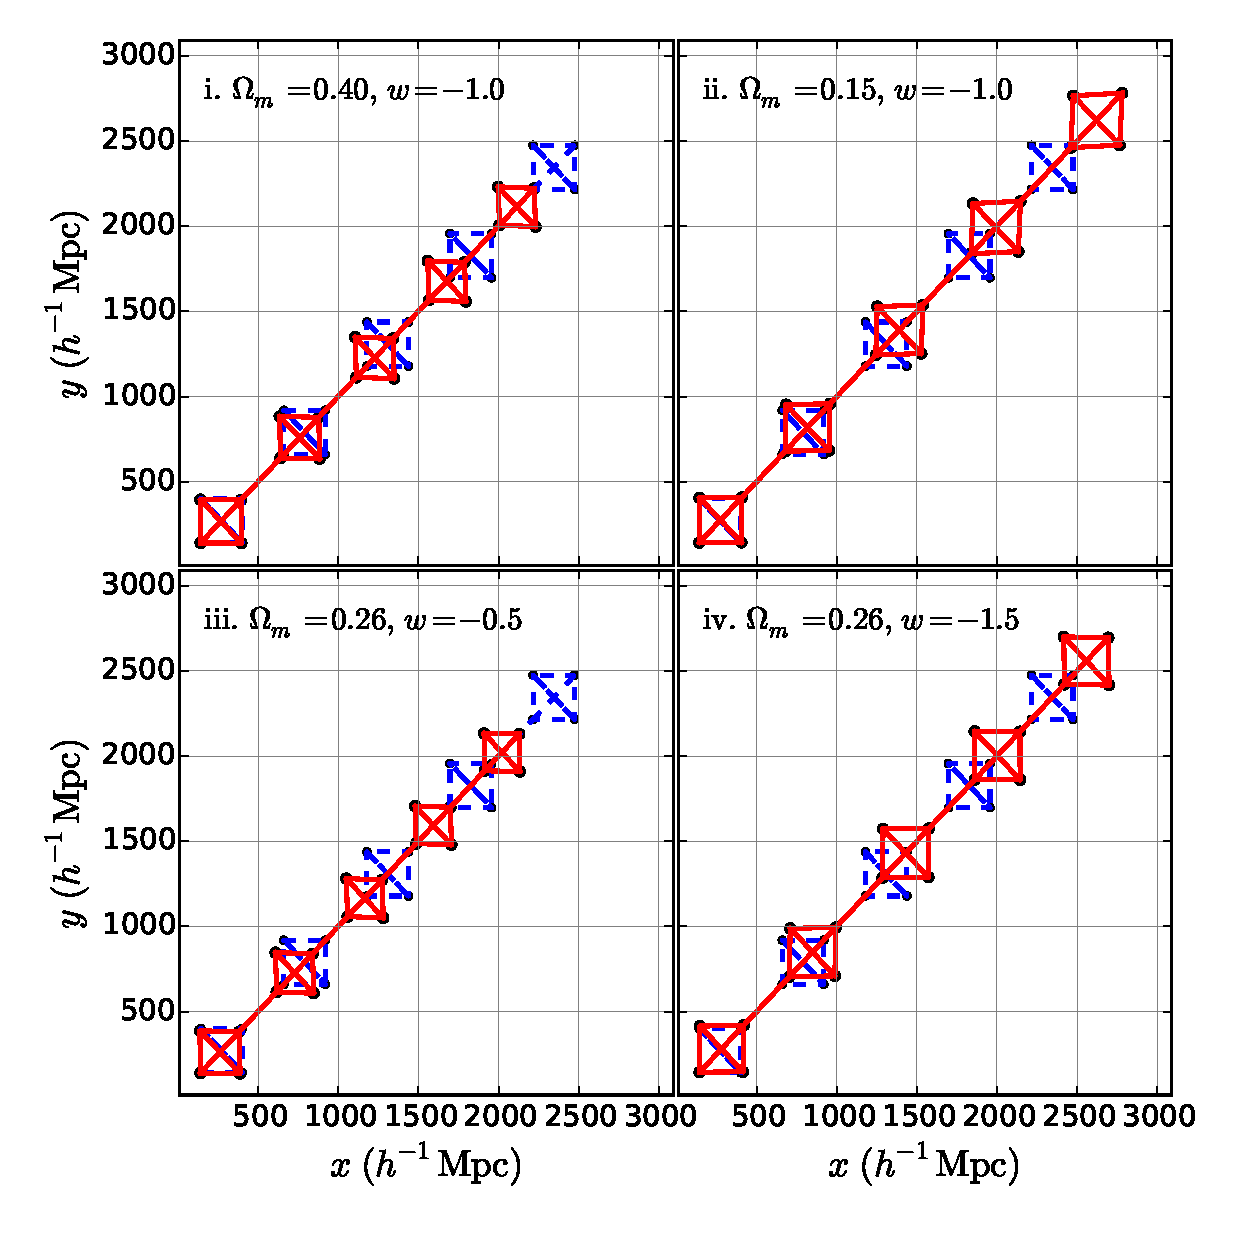
\includegraphics[height=8cm]{fig1_a.eps}
   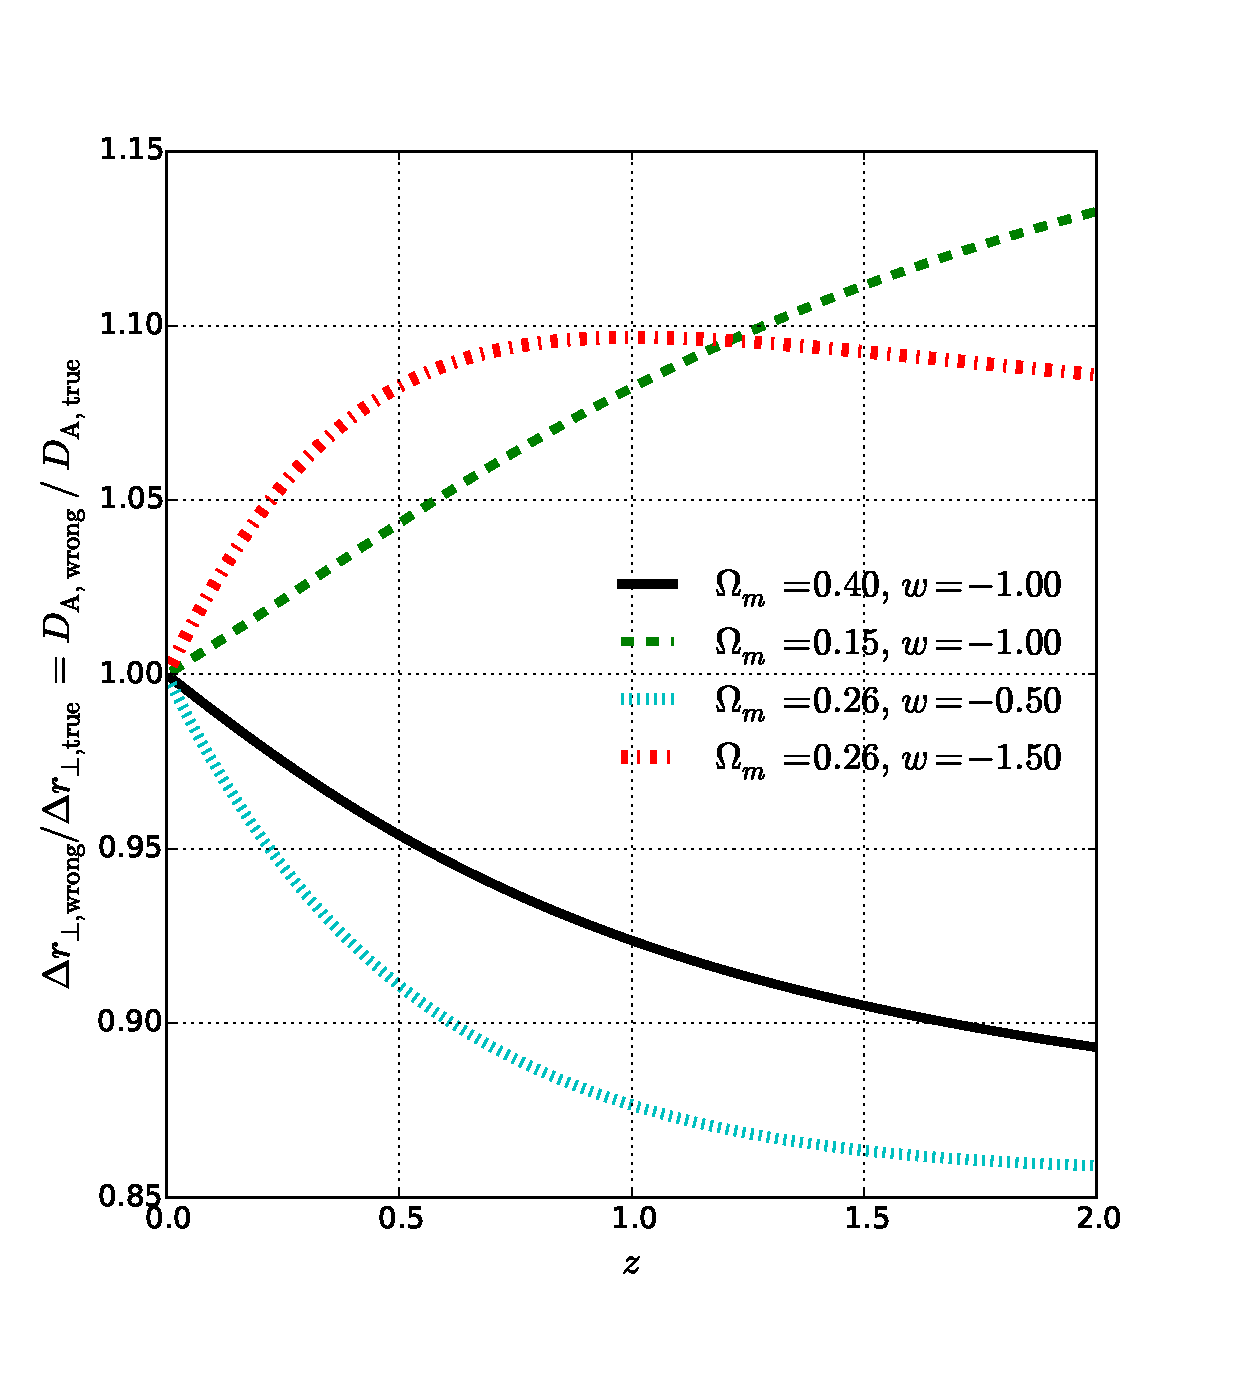
\includegraphics[height=8.5cm]{fig1_b.eps}
   }
   \caption{\label{fig_xyquan}
   %Apparent distortion of objects in four wrongly assumed cosmologies, assuming a true cosmology of .
   The scaling in four wrongly assumed cosmologies ..., % $\Omega_m=0.41$, $w=-1.3$ and $\Omega_m=0.11$, $w=-0.7$, 
   assuming a true cosmology of $\Omega_m=0.26$, $w=-1$.
   Left panel shows a series objects distributes as five perfect squares, measured by an observer located at the origin.
   Their true positions and shapes are plotted in blue dashed lines.
   The observer measures the redshifts of these objects, adopts the wrong cosmologies to compute the distance,
   and obtains wrong results (the red solid lines).
   %The red solid lines show their positions and shapes when the wrong cosmologies 
   % are assumed to compute distance from measured redshift.
   %The misestimation of angular diameter distance lead to wrong 
   Right panel shows the misestimation of angular diameter distance when the wrong cosmologies are adopted.
   %In our mock surveys we split the samples at $z=0.3$, 0.6, 0.9 and 1.2, as marked by the vertical lines.
   %measured by an observer located at the origin.
   %For reference, blue dashed squares show their shapes and positions in the true cosmology.
   }
   % Need a better plot to show angular size variation!!!
\end{figure*}

%Considering we are Let us consider an object in the universe with certain size and shape.
%Its observed redshift span $\Delta z$ and angular size $\Delta \theta$ are related with the comoving sizes by
In this section we briefly introduce the scaling effect in wrongly assumed cosmologies.
A more detailed description has been provided in \cite{Li2014,Li2015,Li2016}.

Suppose that we are probing the shape of some objects in the Universe.
We measure its redshift span $\Delta z$ and angular size $\Delta \theta$,
then compute its sizes in the radial and transverse directions from the relations of 
\begin{equation}\label{eq:distance}
\Delta r_{\parallel} = \frac{c}{H(z)}\Delta z,\ \ \Delta r_{\bot}=(1+z)D_A(z)\Delta \theta,
\end{equation}
where $H$ is the Hubble parameter, $D_A$ is the angular diameter distance.
In the particular case of a flat universe with constant dark energy EoS, they take the forms of
\begin{eqnarray}\label{eq:HDA}
& &H(z) = H_0\sqrt{\Omega_ma^{-3}+(1-\Omega_m)a^{-3(1+w)}},\nonumber\\
& &D_A(z) = \frac{1}{1+z}r(z)=\frac{1}{1+z}\int_0^z \frac{dz^\prime}{H(z^\prime)},
\end{eqnarray}
where $a=1/(1+z)$ is the cosmic scale factor,
$H_0$ is the present value of Hubble parameter and $r(z)$ is the comoving distance.

In case we adopted a wrong set of cosmological parameters in Equation (\ref{eq:distance},\ref{eq:HDA}),
the inferred $\Delta r_{\parallel}$ and $\Delta r_{\bot}$ are wrong,
resulting in distorted shape (AP effect) and wrongly estimated volume (volume effect).
These effects have been discussed in \cite{Li2014,Li2015,Li2016}.
This paper we focus on the misestimation of $\Delta r_{\bot}$,%scaling of angular size,
which can be described by the following quantities
\begin{equation}\label{eq:DA}
 %{\rm Degree\ of\ volume\ magnification \equiv}
 %{\rm rat}_{\rm volume\ mag}\equiv
 \frac{\Delta r_{\bot, \rm wrong}}{\Delta r_{\bot, \rm true}}
 = \frac{D_{A, \rm wrong}}{D_{A, \rm true}},
\end{equation}
where ``true'' and ``wrong'' denote the values of $D_A$ in the true cosmology and wrongly assumed cosmology.

The effects due to wrongly assumed cosmological parameters are shown in the upper panel of Figure \ref{fig_xyquan}.
Suppose that the true cosmology is a flat $\Lambda$CDM with present density parameter $\Omega_m=0.26$
and standard dark energy EoS $w=-1$.
If we were to distribute a series of perfect squares at various distances from 500 Mpc/h to 3\,000 Mpc/h,
and an observer located at the origin were to measure their redshifts and compute their positions and shapes 
using redshift-distance relations of four incorrect cosmologies
\begin{eqnarray}
 & &{\rm (i)}.\ \Omega_m=0.40,\ w=-1.0, \nonumber \\ 
 & &{\rm (ii)}.\ \Omega_m=0.15,\ w=-1.0, \nonumber\\ \noindent
 & &{\rm (iii)}.\ \Omega_m=0.26,\ w=-0.5,\nonumber\\ \noindent
 & &{\rm (iv)}.\ \Omega_m=0.26,\ w=-1.5, \nonumber \noindent
\end{eqnarray}
the shapes of the squares appear distorted (AP effect),
and their volumes are changed (volume effect).
In the cosmological models in model (i,iii) we see a compression of size (in both angular and LOS direction)
and the degree of compression increases with increasing distance,
while in models (ii,iv) we see stretch of size whose degree also evolves with redshift.
Thus, when wrong cosmological parameters are adopted,
the apparent size of objects are distorted, and the magnitude of distortion also varies with redshift.

In this paper we will use the galaxy angular 2pCF to probe the redshift dependence of the distortion in angular direction.
In the right panel of Figure \ref{fig_xyquan} we plot the redshift dependence of the change in angular size, 
${\Delta r_{\bot, \rm wrong}}/{\Delta r_{\bot, \rm true}}$, in the four wrong cosmologies.
In all cosmologies, there is clear evolution of ${\Delta r_{\bot, \rm wrong}}/{\Delta r_{\bot, \rm true}}$ 
in the redshift range $0<z<2$.
E.g., when use the quintessence cosmology 
$\Omega_m=0.26,\ w=-0.5$ to infer the postions of objects,
the angular size is underestimated by 
%12.5\%, 17.7\%, 20.1\%, 21.3\%
8.9\%, 12.3\%, 13.6\%, 14.1\% 
at $z=0.5,1,1.5,2$.




\section{The Simulation Data}\label{sec:data}

We test the method on the Horizon Run 4  (HR4) simulation \citep{hr4}.
HR4 used $N=6300^3$ particles in a box size of $L={3150}$ $h^{-1}$Mpc.  
It adopted the second order Lagrangian perturbation theory (2LPT) initial conditions at $z_{i}=100$
and a WMAP5 cosmology $(\Omega_{b},\Omega_{m},\Omega_\Lambda,h,\sigma_8,n_s)$  = (0.044, 0.26, 0.74, 0.72, 0.79, 0.96) \citep[]{komatsu 2011}.
The particle mass is $\simeq m_{p} \simeq 9.02 \times 10^9 \hMsun$.
%This starting redshift, combined  with 2LPT initial conditions, ensures an accurate mass function and power spectrum \citep{2014NewA...30...79L}. 

Mock galaxy samples are produced from the simulation based on a modified one-to-one correspondence scheme \citep{hong2016}. 
The most bound member particles (MBPs) of simulated halos are adopted as the tracer of galaxies,
and the merger timescale is computed to get the lifetime of merged halos.
Merger trees of simulated halos are constructed by tracking their MBPs from $z = 12$ to 0.
When a merger event occurs, we adopt the formular of \cite{jiang2008} to calculate the merger timescale 
and determine when a satellite galaxy is completely disrupted.
%We modeled the position and the velocity of a galaxy from the position and velocity of its corresponding MBP.
%By using the abundance matching, 
%we modeled the luminosity of a central/isolated galaxies from their current mass
%and of satellite galaxies from their mass at the time of infall.

\cite{hong2016} compared the 2pCF of the SDSS DR7 volume-limited galaxy sample \citep{zehavi2011} and the HR4 $z=0$ mock galaxies.
%When a typical subhalo-galaxy correspondence scheme is applied, 
%the 2pCF from our simulation is smaller than the observation and does not show a proper Finger-of-God (FOG) feature in our simulation resolution. 
%We found that %the %2pCF of our galaxy sample agrees well with the observation.
The mock galaxies shows a similar finger of god (FOG) feature \citep{FOG} as the observation.
On scales greater than 1 ${h^{-1}}$Mpc., 
the projected 2pCF of the mock and observational samples agree within 1$\sigma$ deviation.

%As will be introduced in the next section, 
The output of HR4 simulation includes one all-sky light cone mock galaxy catalogue reaching $r=3\,150$ ${h^{-1}}$Mpc 
and a series ({\bf how many?}) of snapshot mock galaxy catalogues at different redshifts.
In this paper we use five snapshot data at $z=0,0.5,1,1.5,2$.
We require subhalos to have at least 30 member particles, 
so the minimal mass of galaxies is $\simeq m_{p} \simeq 2.7 \times 10^{11} \hMsun$.
At the five redshifts, we get a number of
%$4.57\times 10^8$, $4.06\times 10^8$, $3.52\times 10^8$, $3.06\times 10^8$ and $2.28 \times 10^8$ mock galaxies,
457, 406, 352, 206 and 228 million mock galaxies,
corresponding to a number density of 
%$1.46\times 10^{-2}$, $1.30\times 10^{-2}$, $1.13\times 10^{-2}$, $0.98\times 10^{-2}$ and $0.73\times 10^{-2}\ (h^{-1} \rm Mpc)^{-3}$,
1.46, 1.30, 1.13, 0.98 and 0.73 in unit of $ 10^{-2} h^{3} \rm Mpc^{-3}$,
%$1.46\times 10^{-2}$, $1.30\times 10^{-2}$, $1.13\times 10^{-2}$, $0.98\times 10^{-2}$ and $0.73\times 10^{-2}\ (h^{-1} \rm Mpc)^{-3}$,
respectively.

\section{Galaxy angular 2pCF}

\subsection{Galaxy distribution at different redshifts}

The left panels of Figure \ref{fig_scatter} show the $x,y$ coordinates of galaxies in a 
$260 h^{-1} {\rm Mpc} \times 130 h^{-1} {\rm Mpc} \times 105 h^{-1} {\rm Mpc}$ volume, 
taken from the five snapshots.
The gravitational growth of structures with decreasing redshift is clearly shown.
We display all mock galaxies with $M> 3.0 \times 10^{11} \hMsun$.
At lower redshift, galaxies become more massive, so they are more galaxies satisfying the threshold.

If one adopts a wrong cosmology to compute galaxy positions, there would be a scaling of the galaxy distribution.
In the left panel we show the case when a wrong set of parameters $\Omega_m=0.05,\ w=-1.5$ is assumed,
leading to large upscaling of $25.6\%,47.3\%,62.2\%,71.7\%$ at redshifts $z=0.5,1.0,1.5,2.5$.

Compared with the true galaxy distribution, the apparent distribution inferred by wrong set of parameters
show clear evolution with redshift due to the different scaling at different redshifts.
In case of Figure \ref{fig_scatter}, the apparent size of large scale structures increases with redshift.

The growth of structure also make the size of structures evolves with redshift.
In the next subsection we will discuss how to distinguish these two effects in the galaxy angular 2pCF.


\begin{figure*}
   \centering{
   %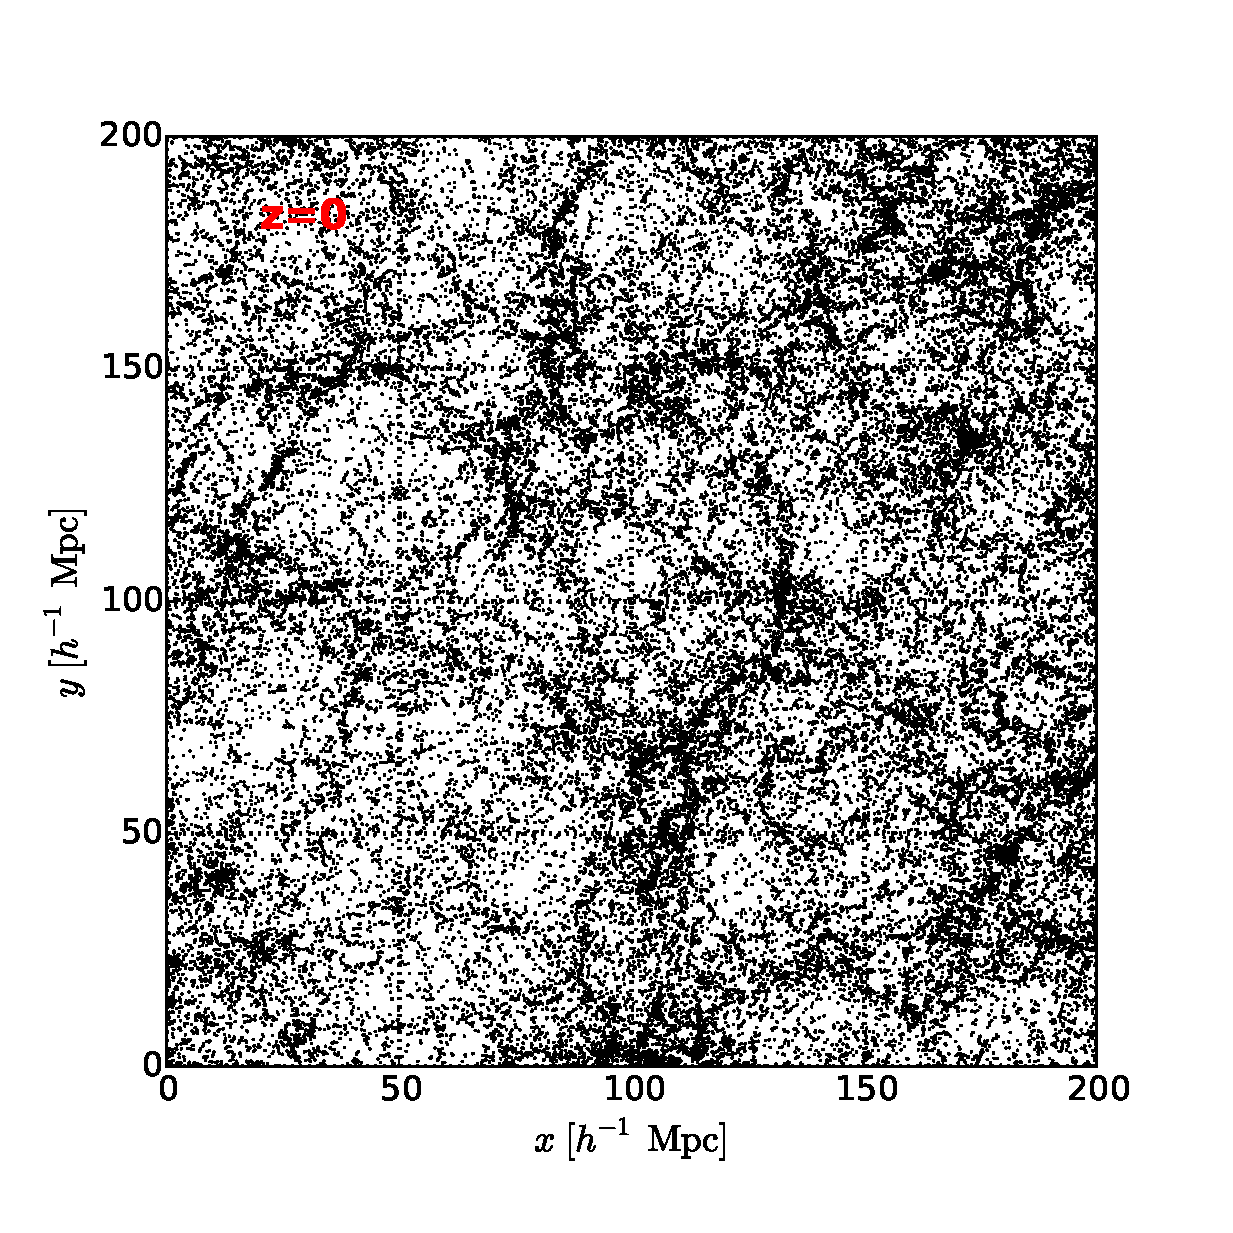
\includegraphics[height=5.9cm]{fig8_0.eps}
   %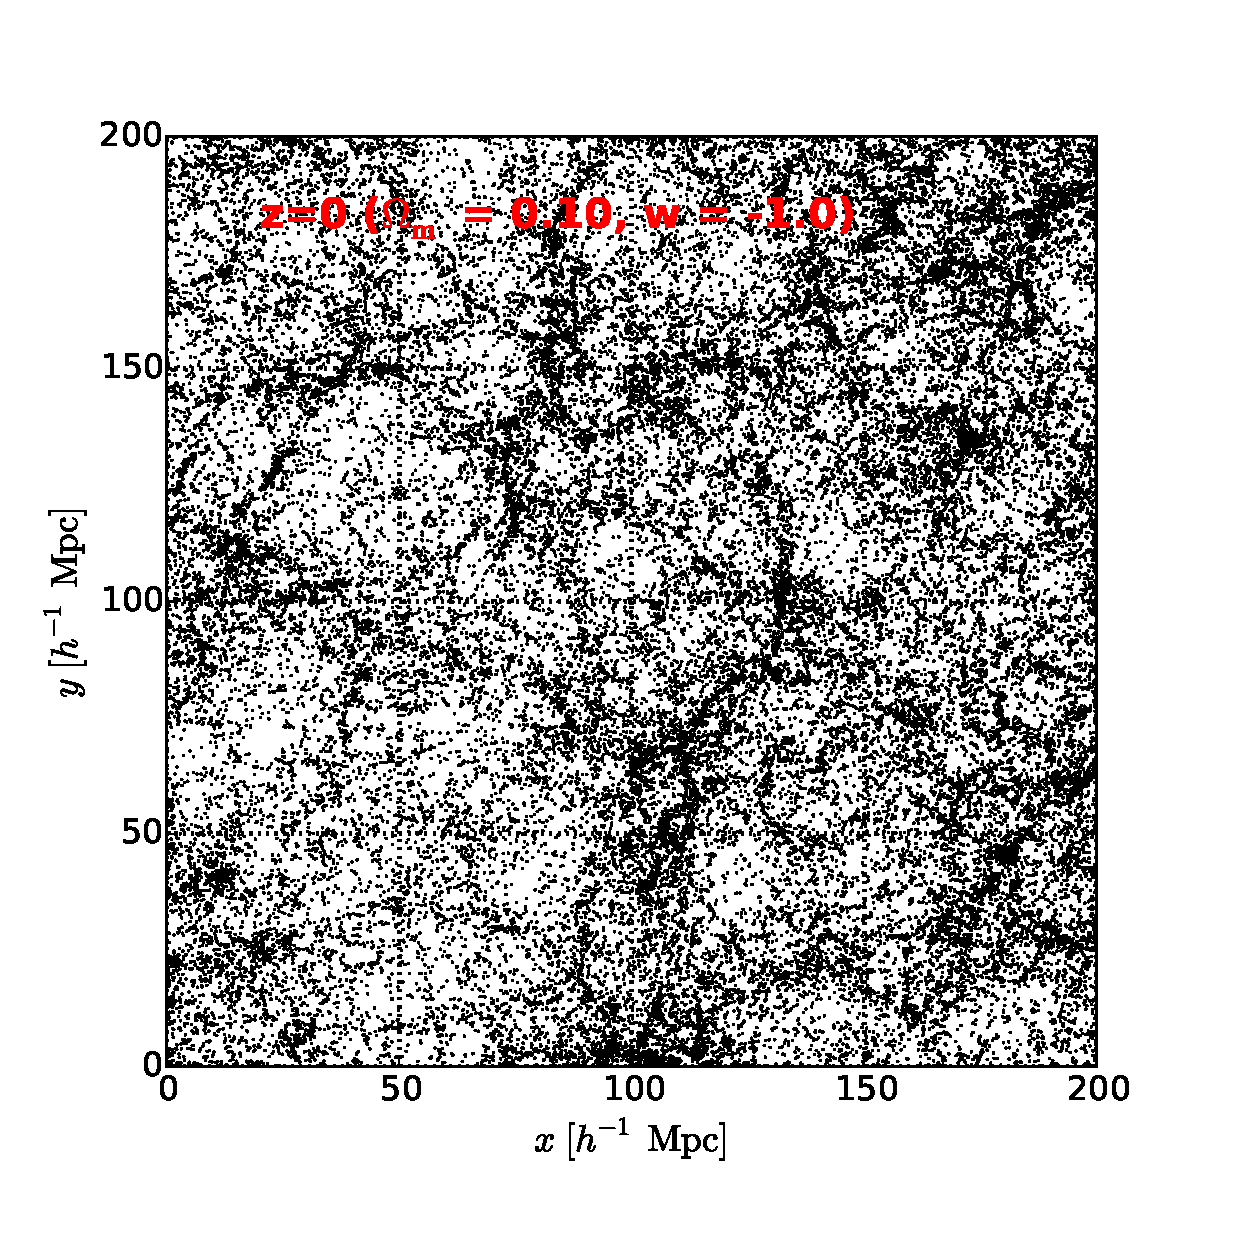
\includegraphics[height=5.9cm]{fig8_wrongcos_0.eps}
   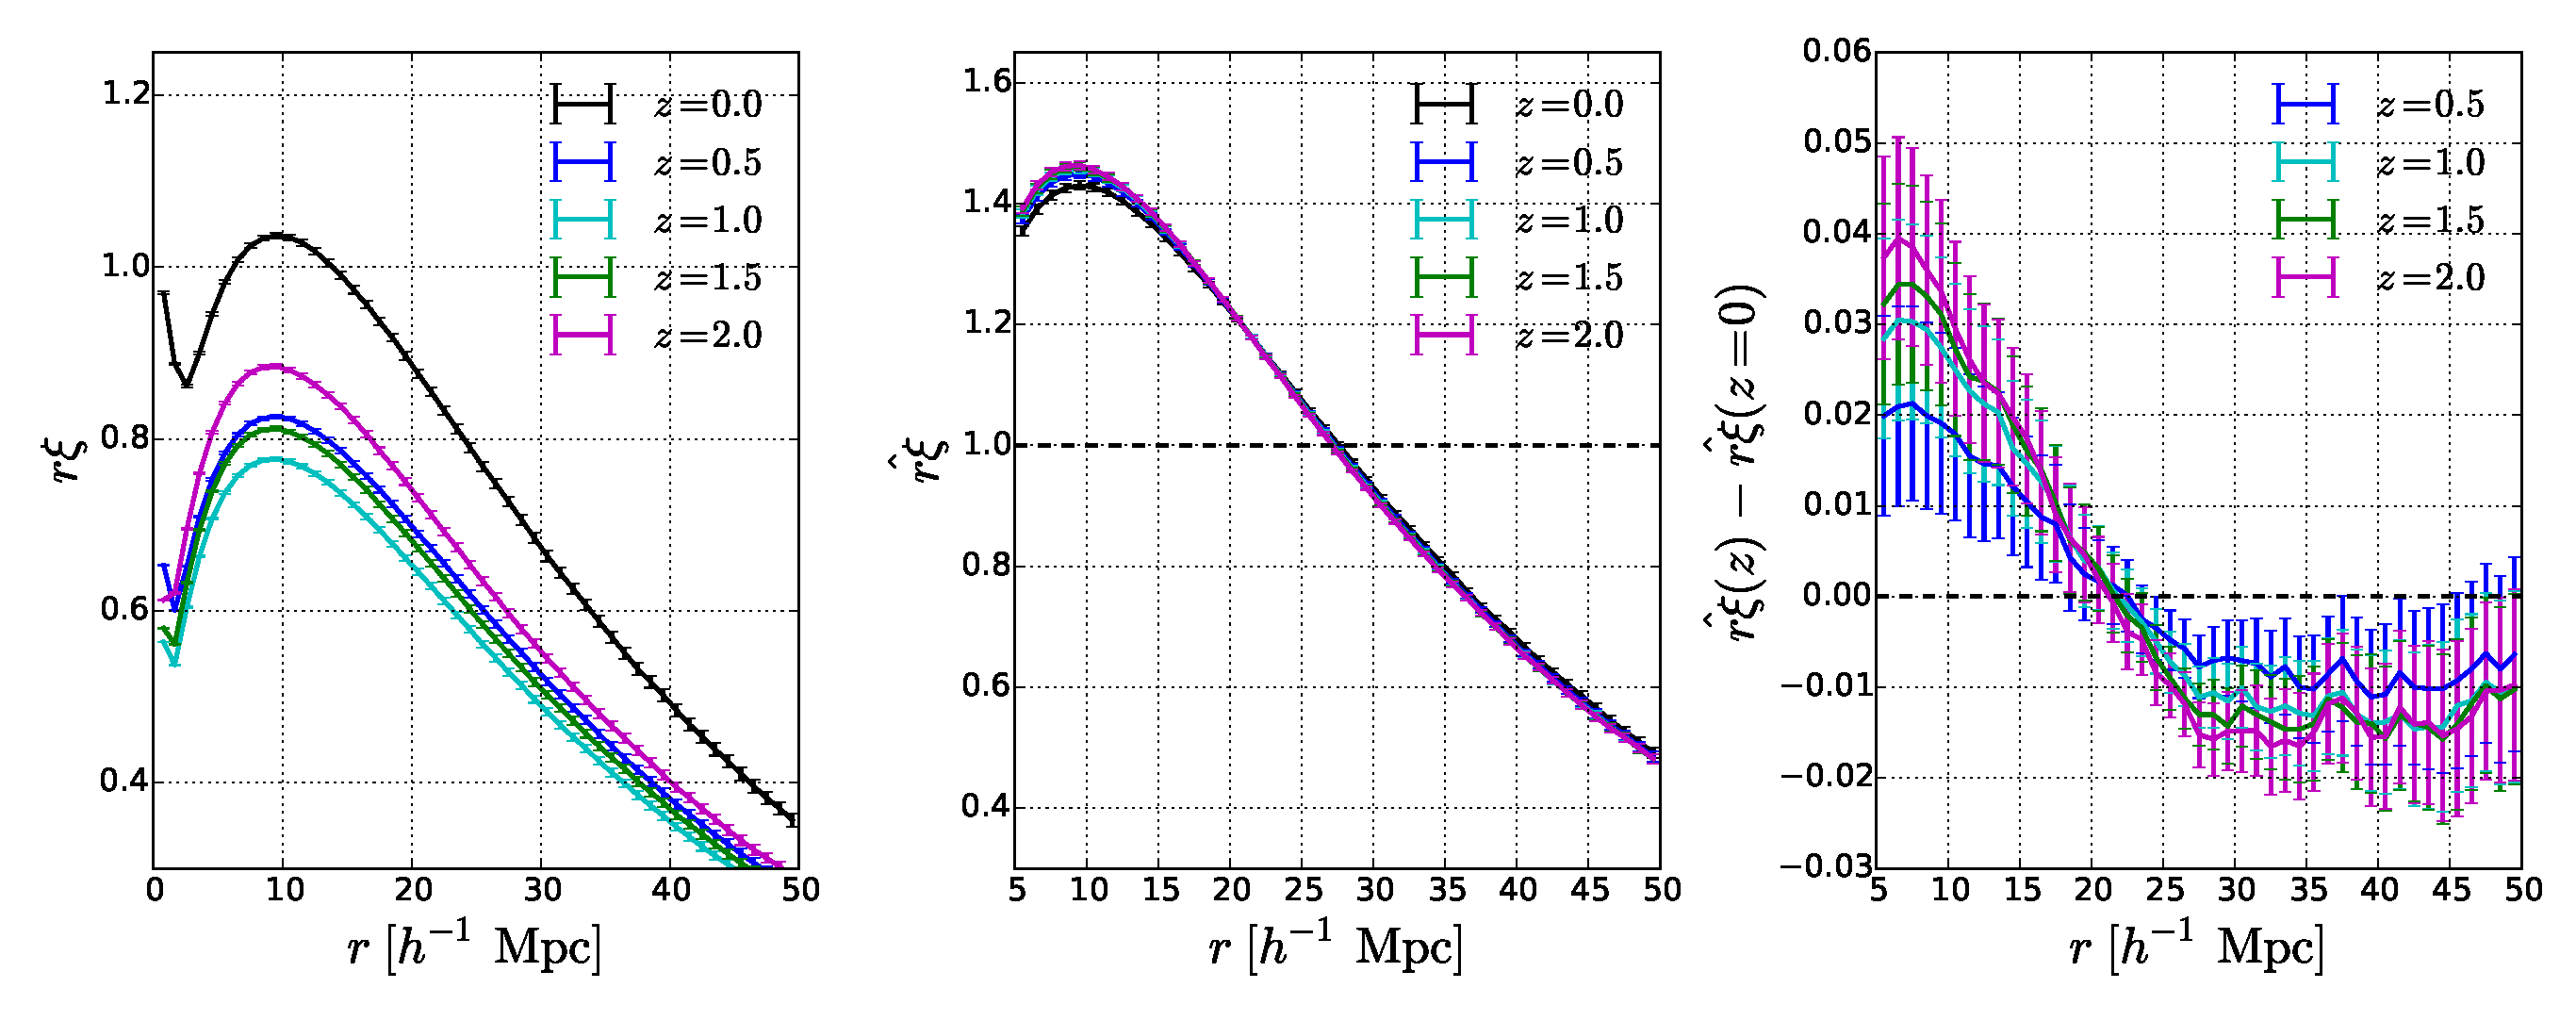
\includegraphics[width=16cm]{fig2.eps}
   }
   \caption{\label{fig_scatter}
  blah
   }
   % Need a better plot to show angular size variation!!!
\end{figure*}

\subsection{Galaxy angular 2pCF at different redshifts}

\begin{figure*}
   \centering{
%   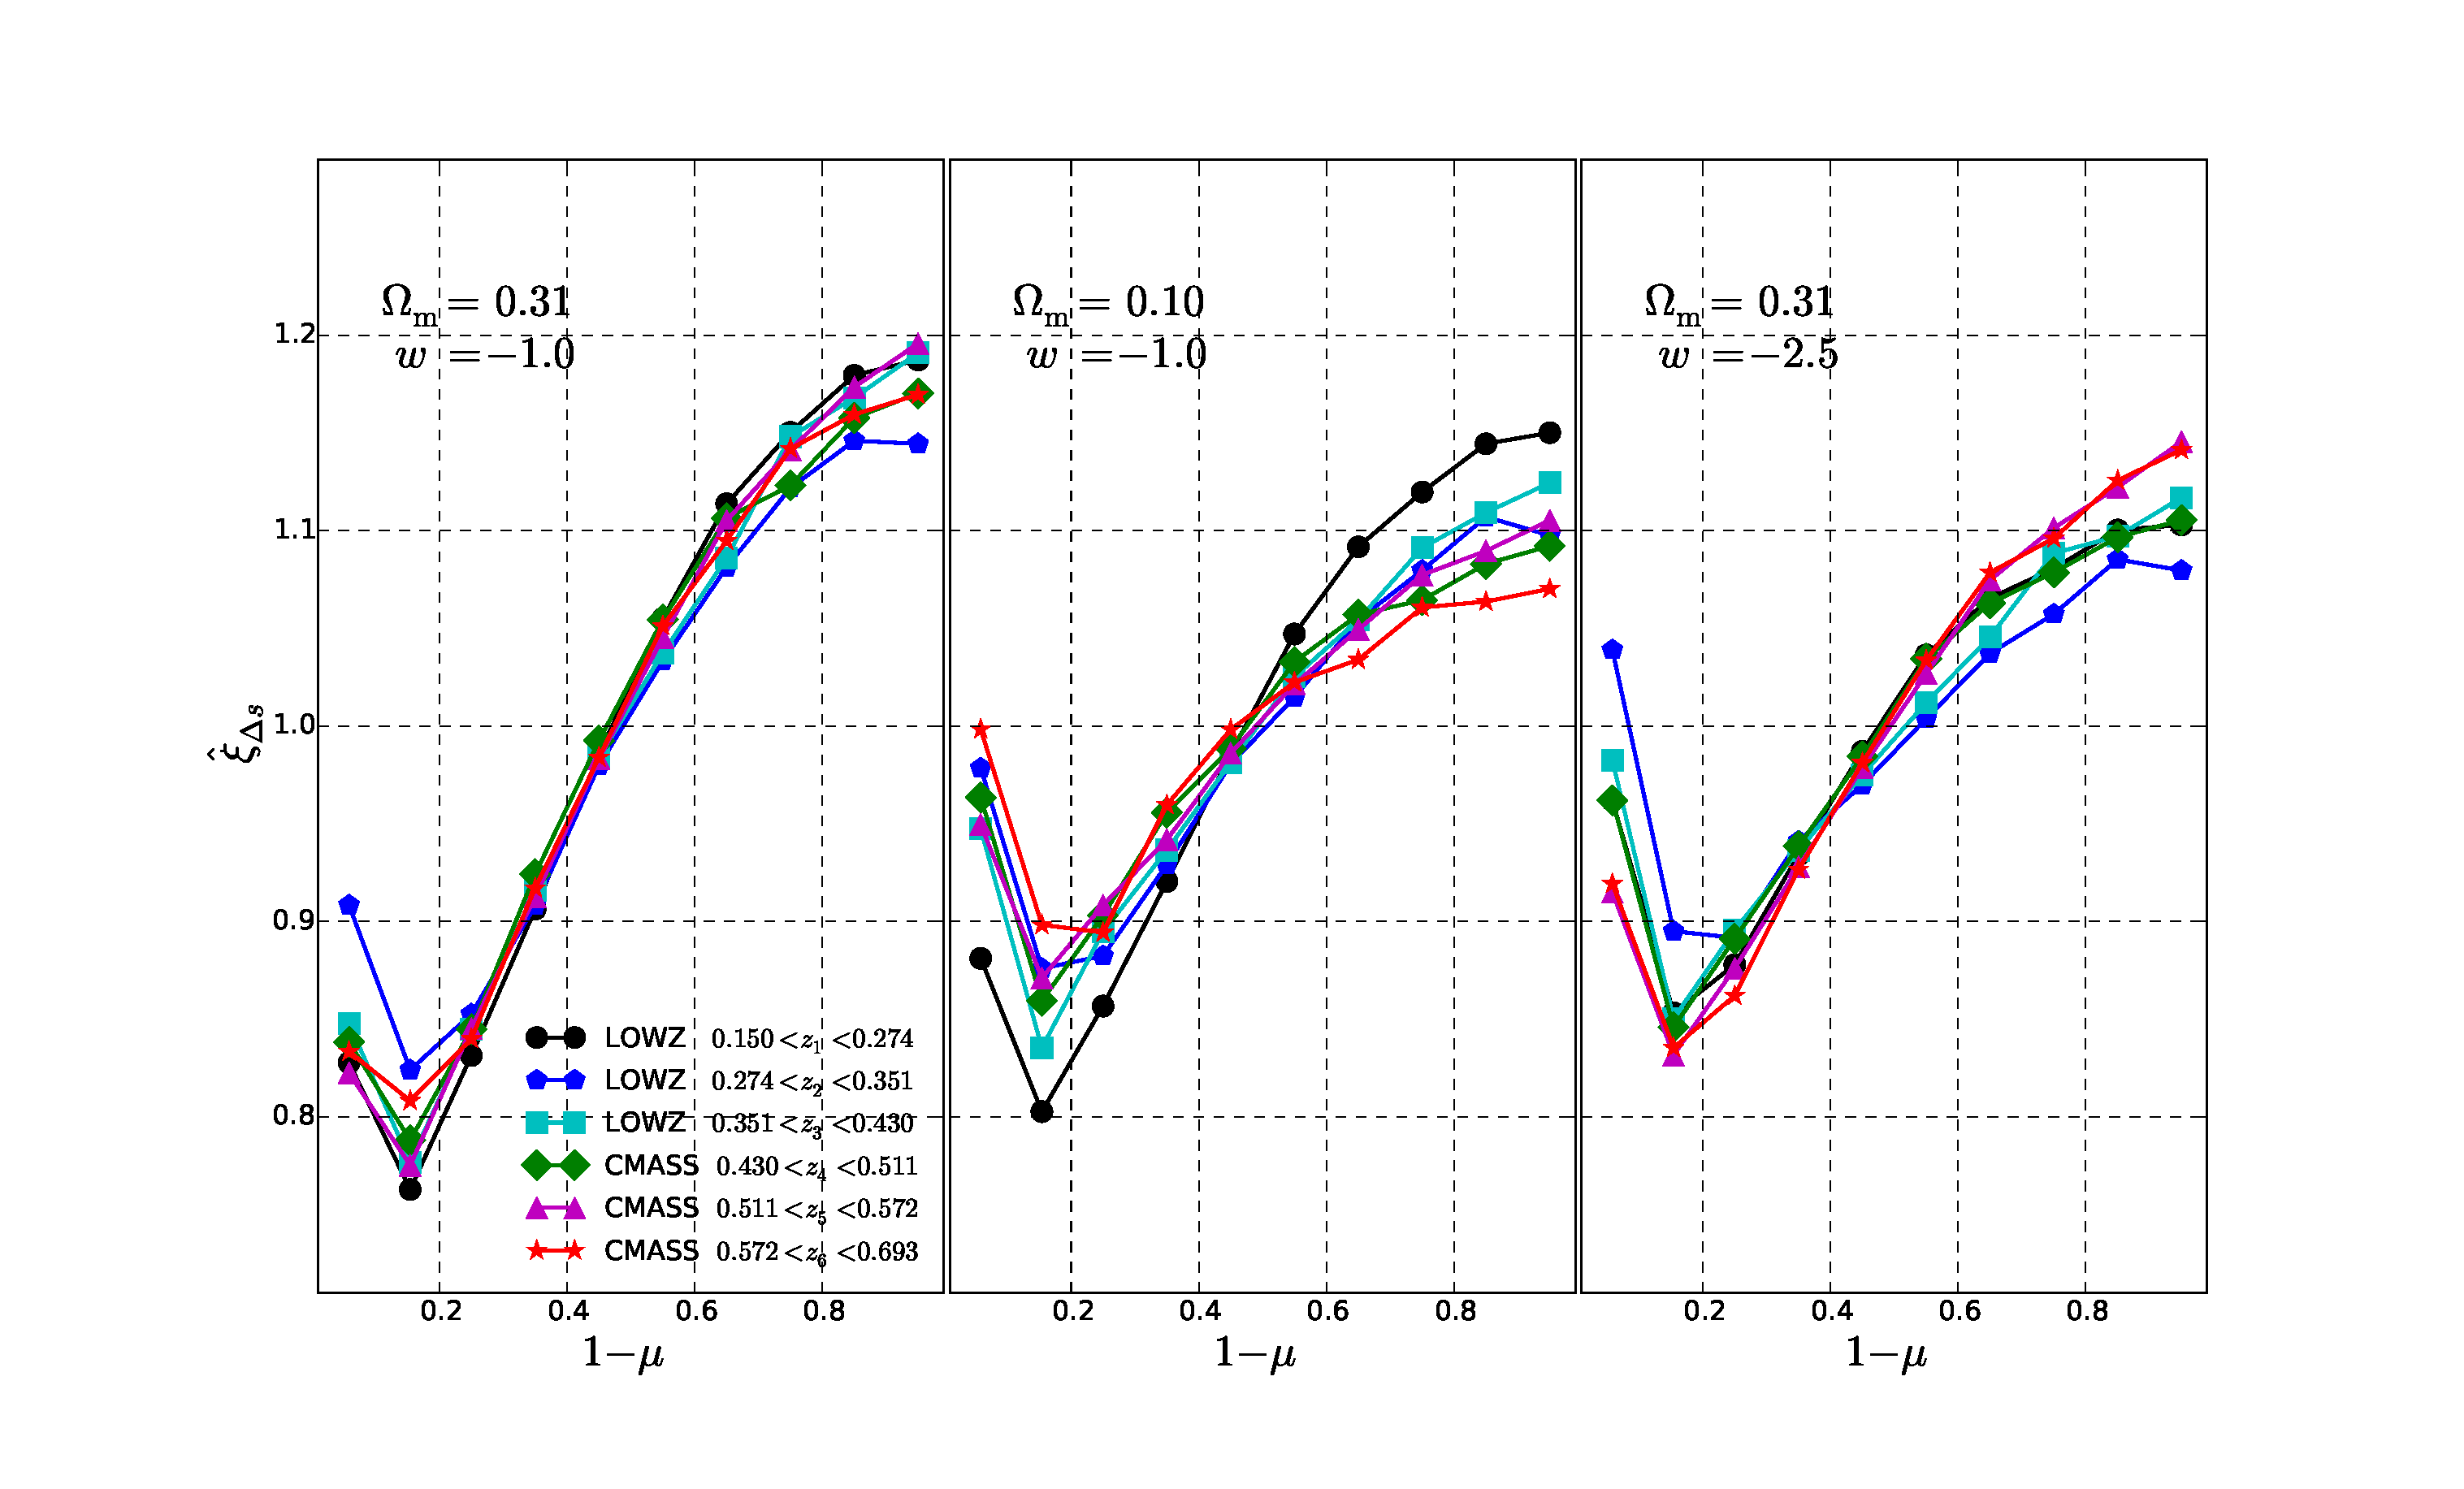
\includegraphics[width=18cm]{fig9_0.eps}
%   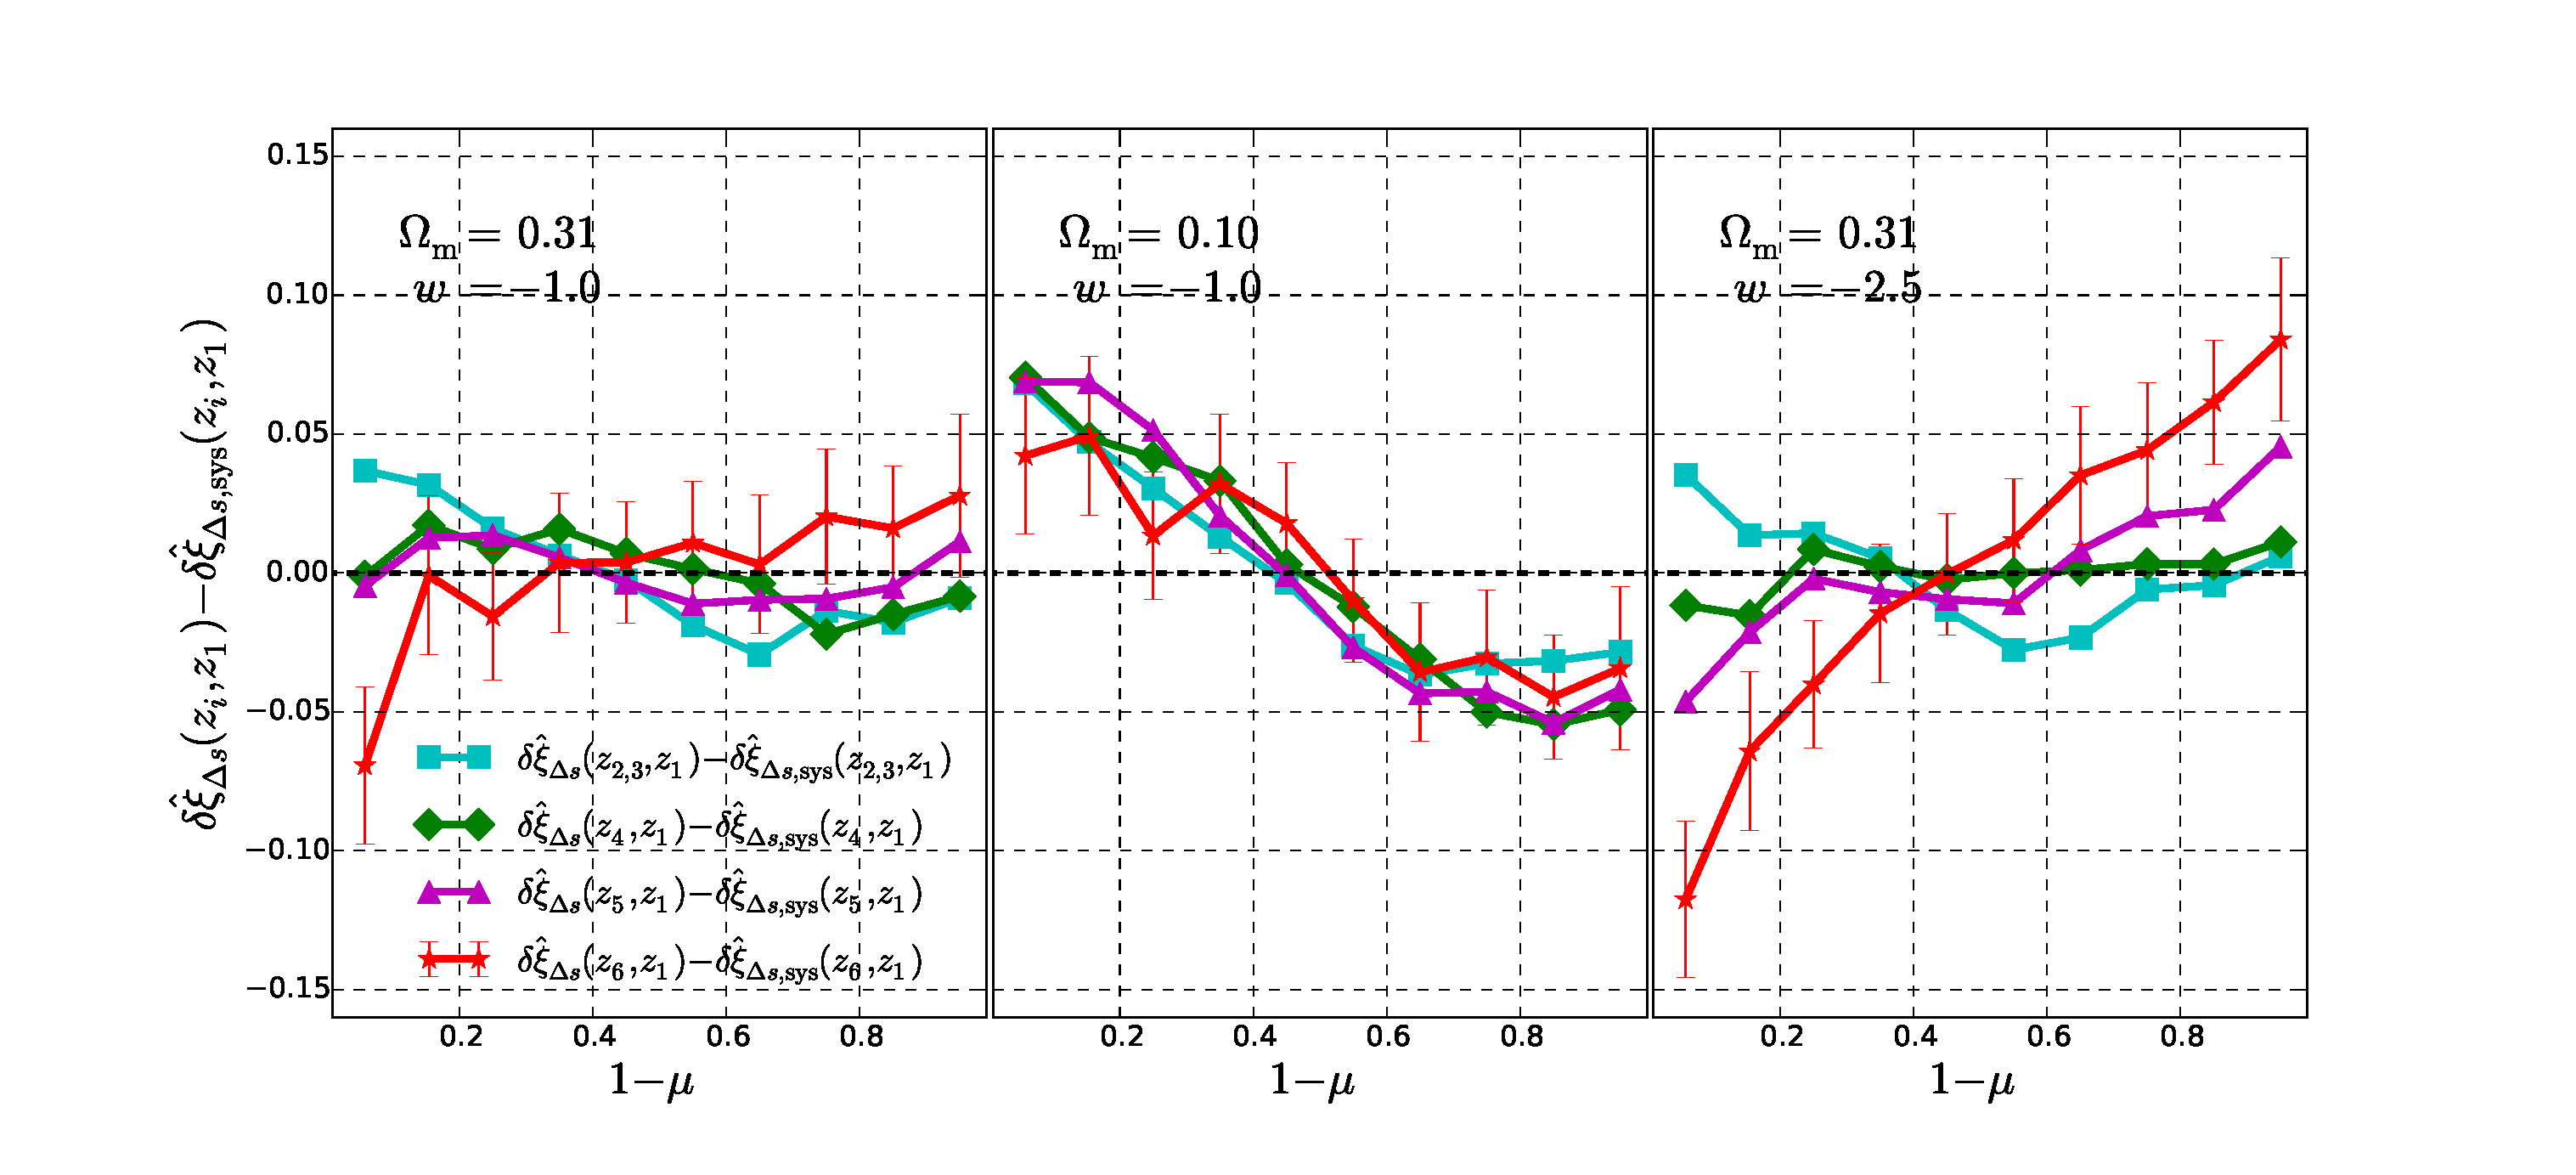
\includegraphics[width=18cm]{fig9_1.eps}
%   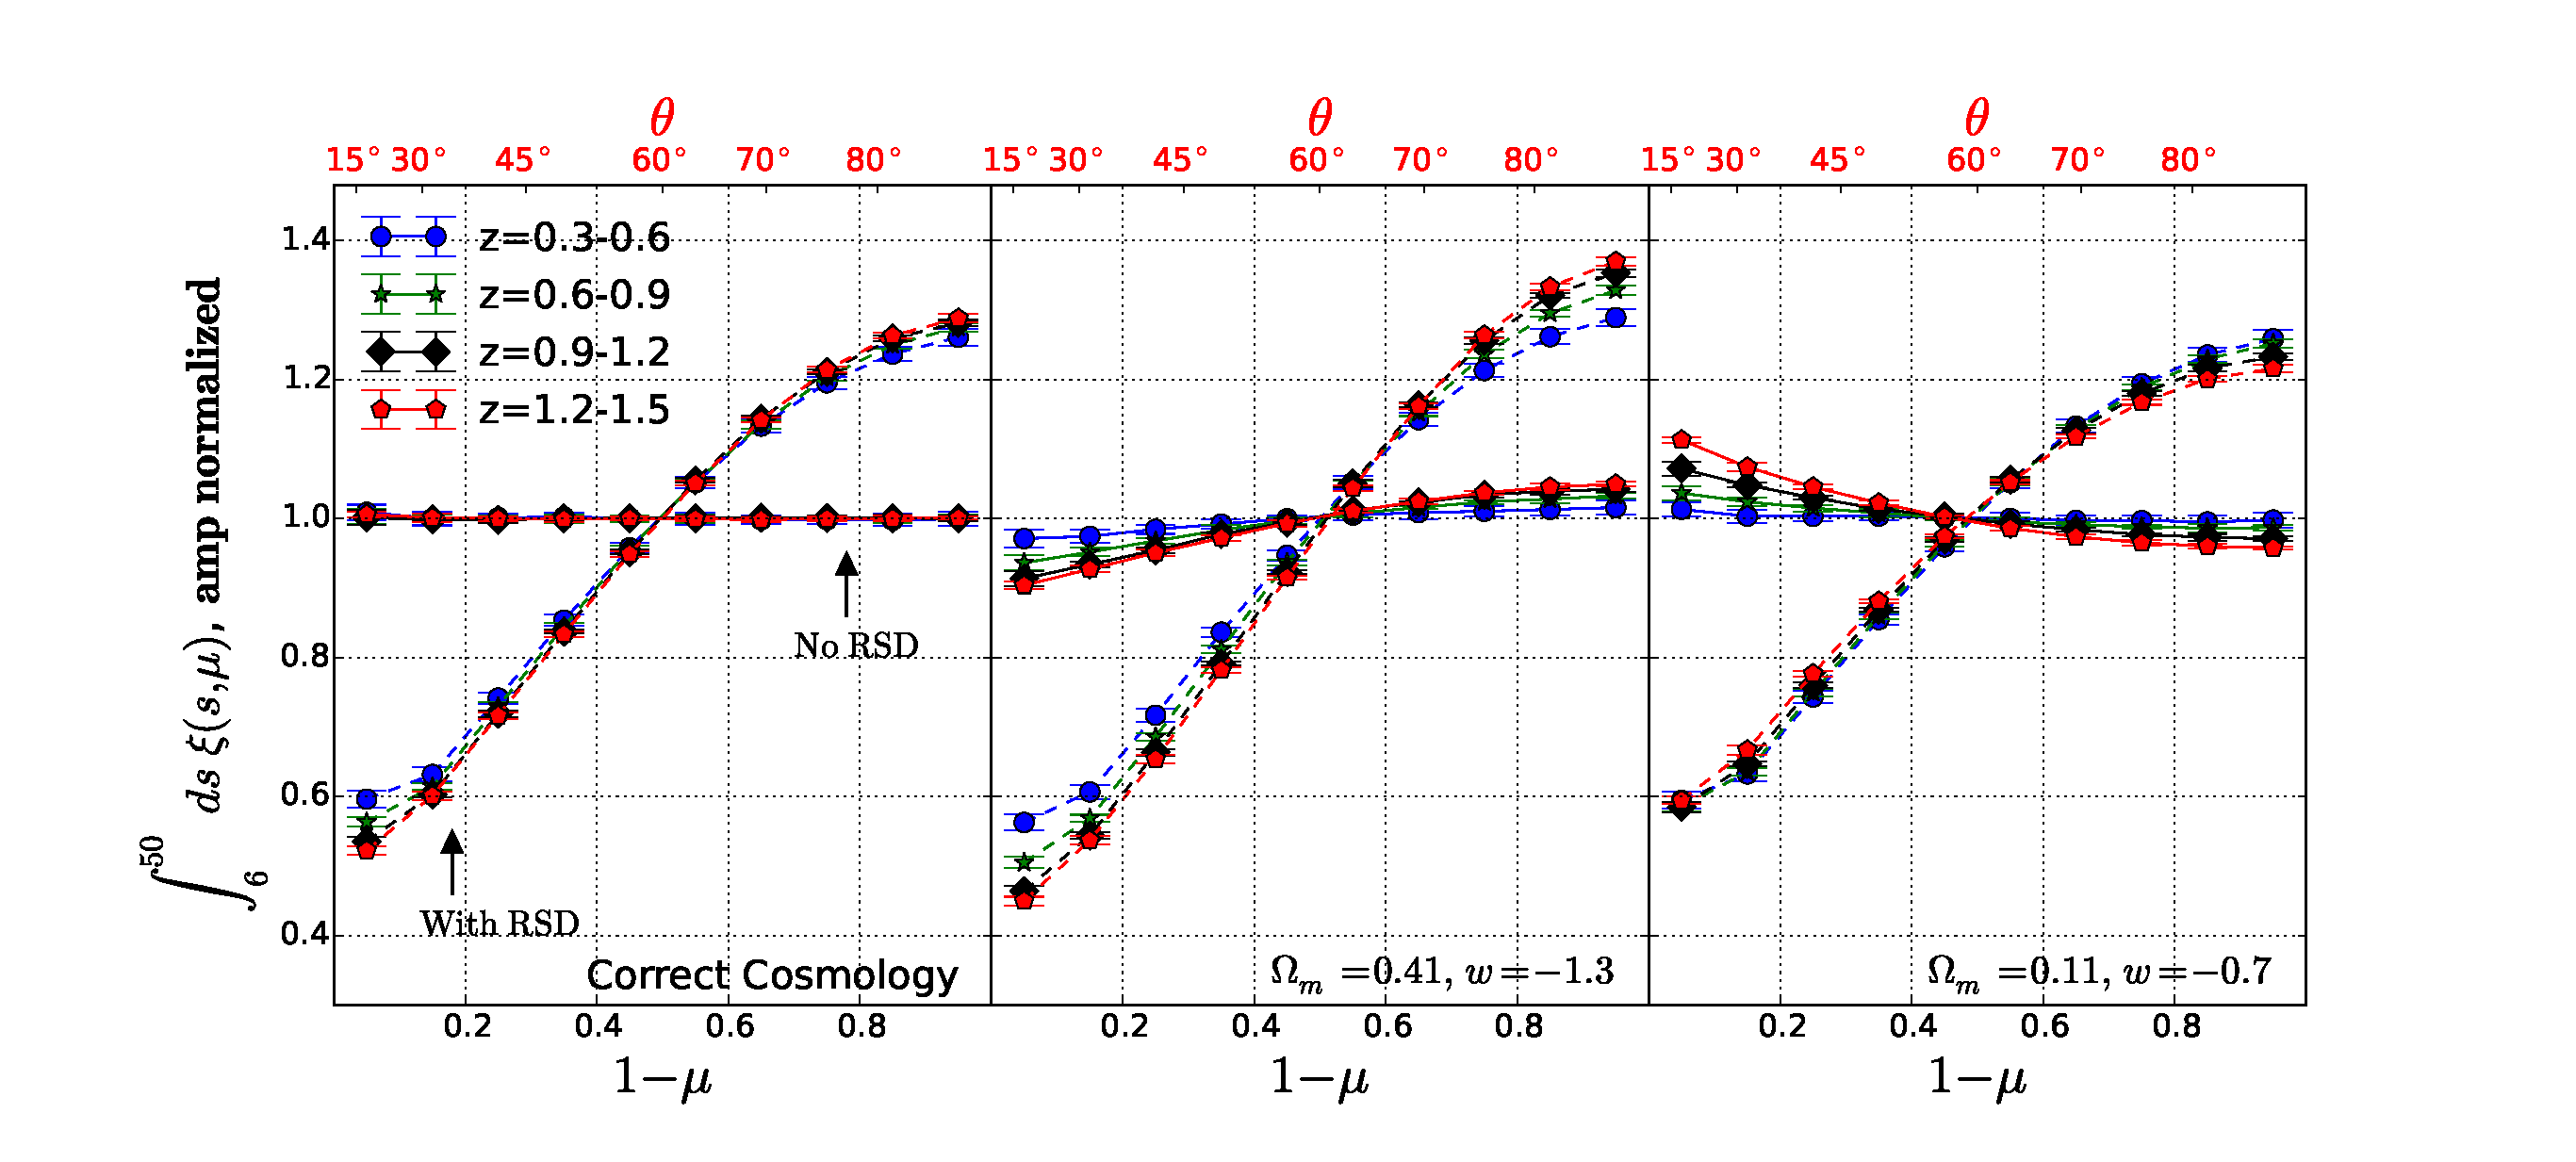
\includegraphics[height=8cm]{Tpcf--plot--Normed.eps}
%    \includegraphics[height=8cm]{smu.eps}
    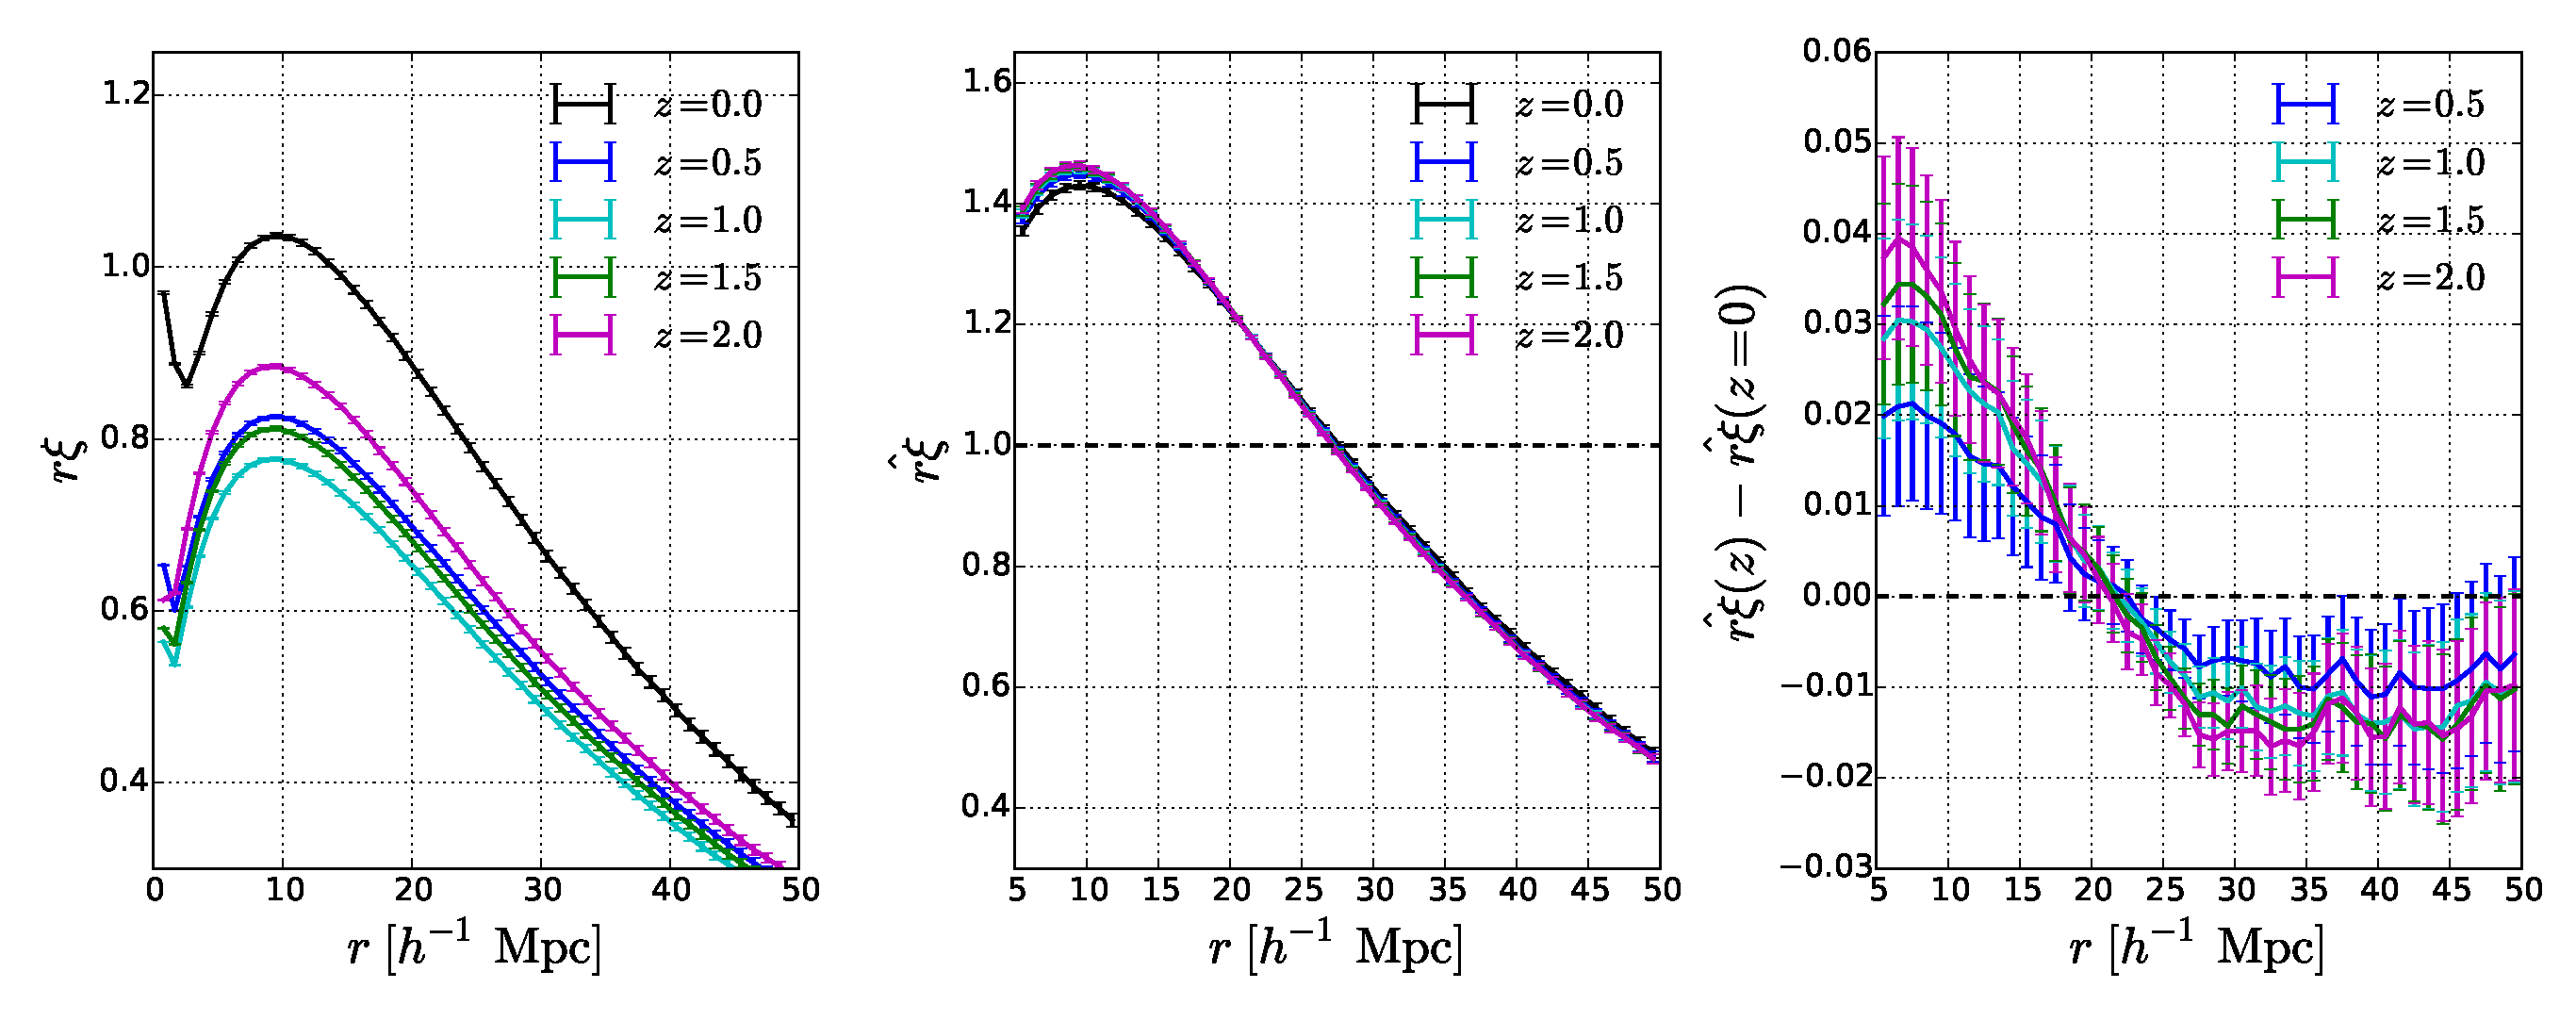
\includegraphics[width=18cm]{fig2.eps}
   }
   \caption{\label{fig_diffz}
  2pCF at different redshfits.
   }
\end{figure*}

\begin{figure*}
   \centering{
%   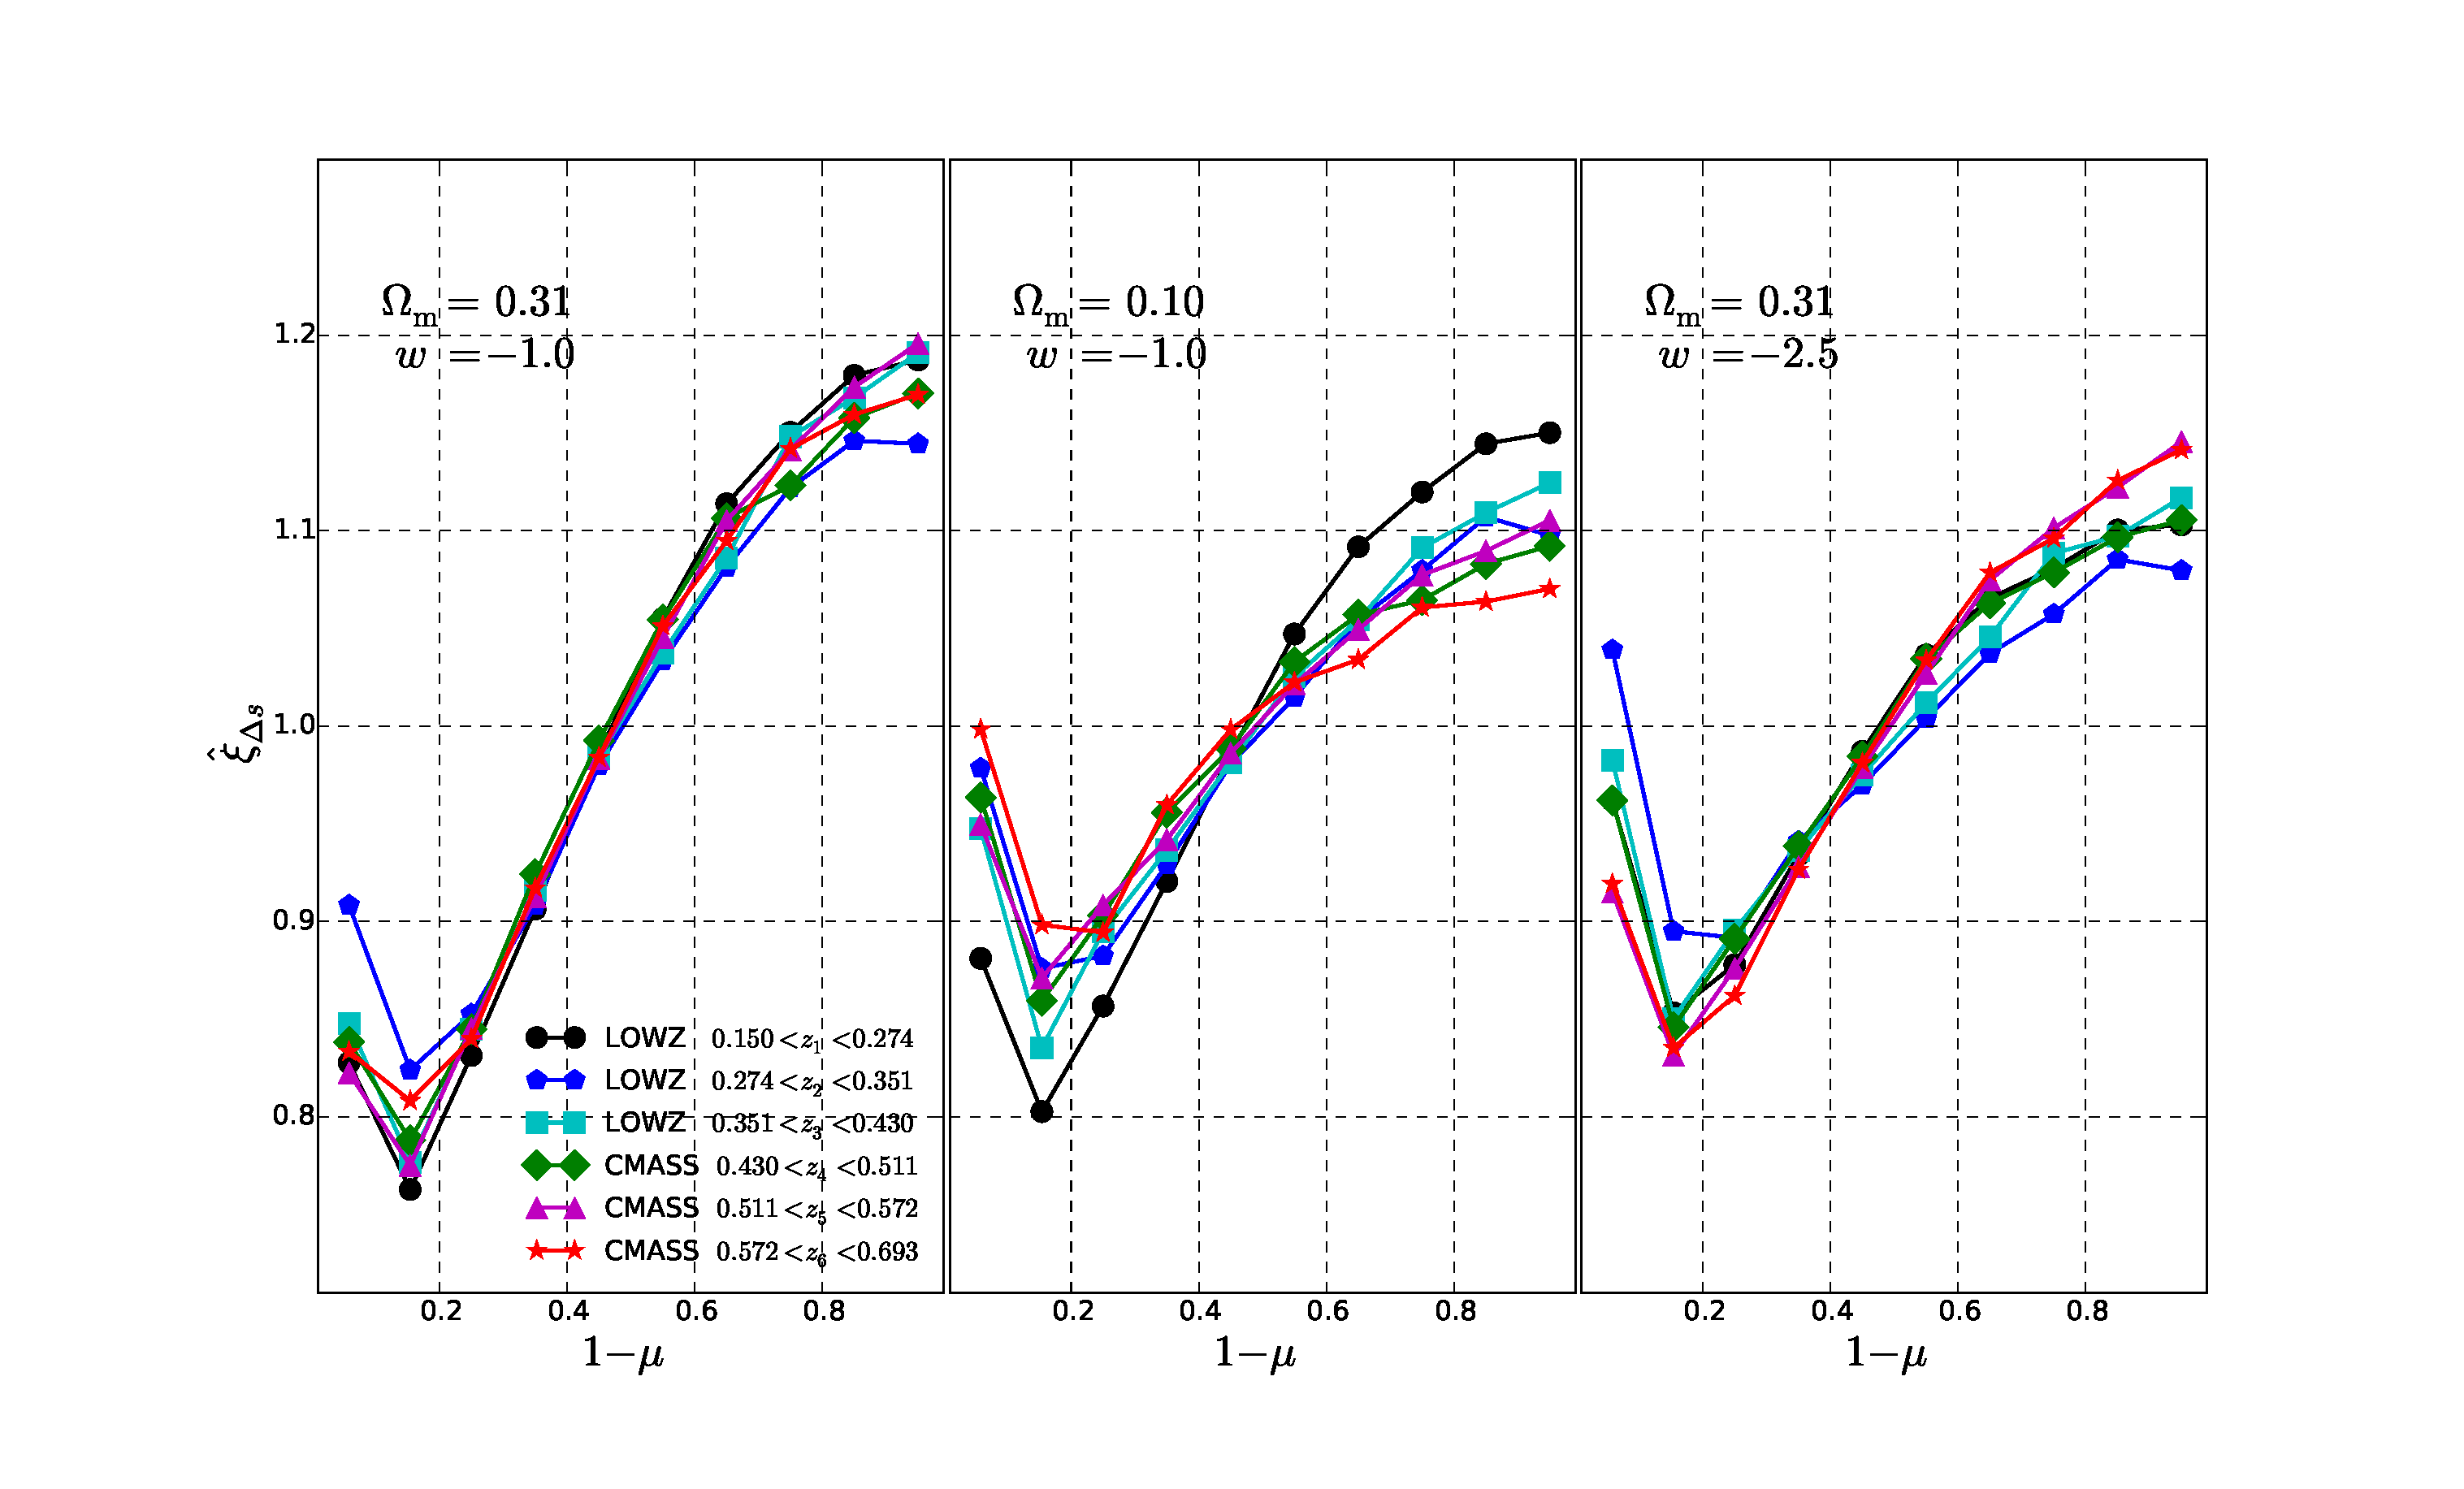
\includegraphics[width=18cm]{fig9_0.eps}
%   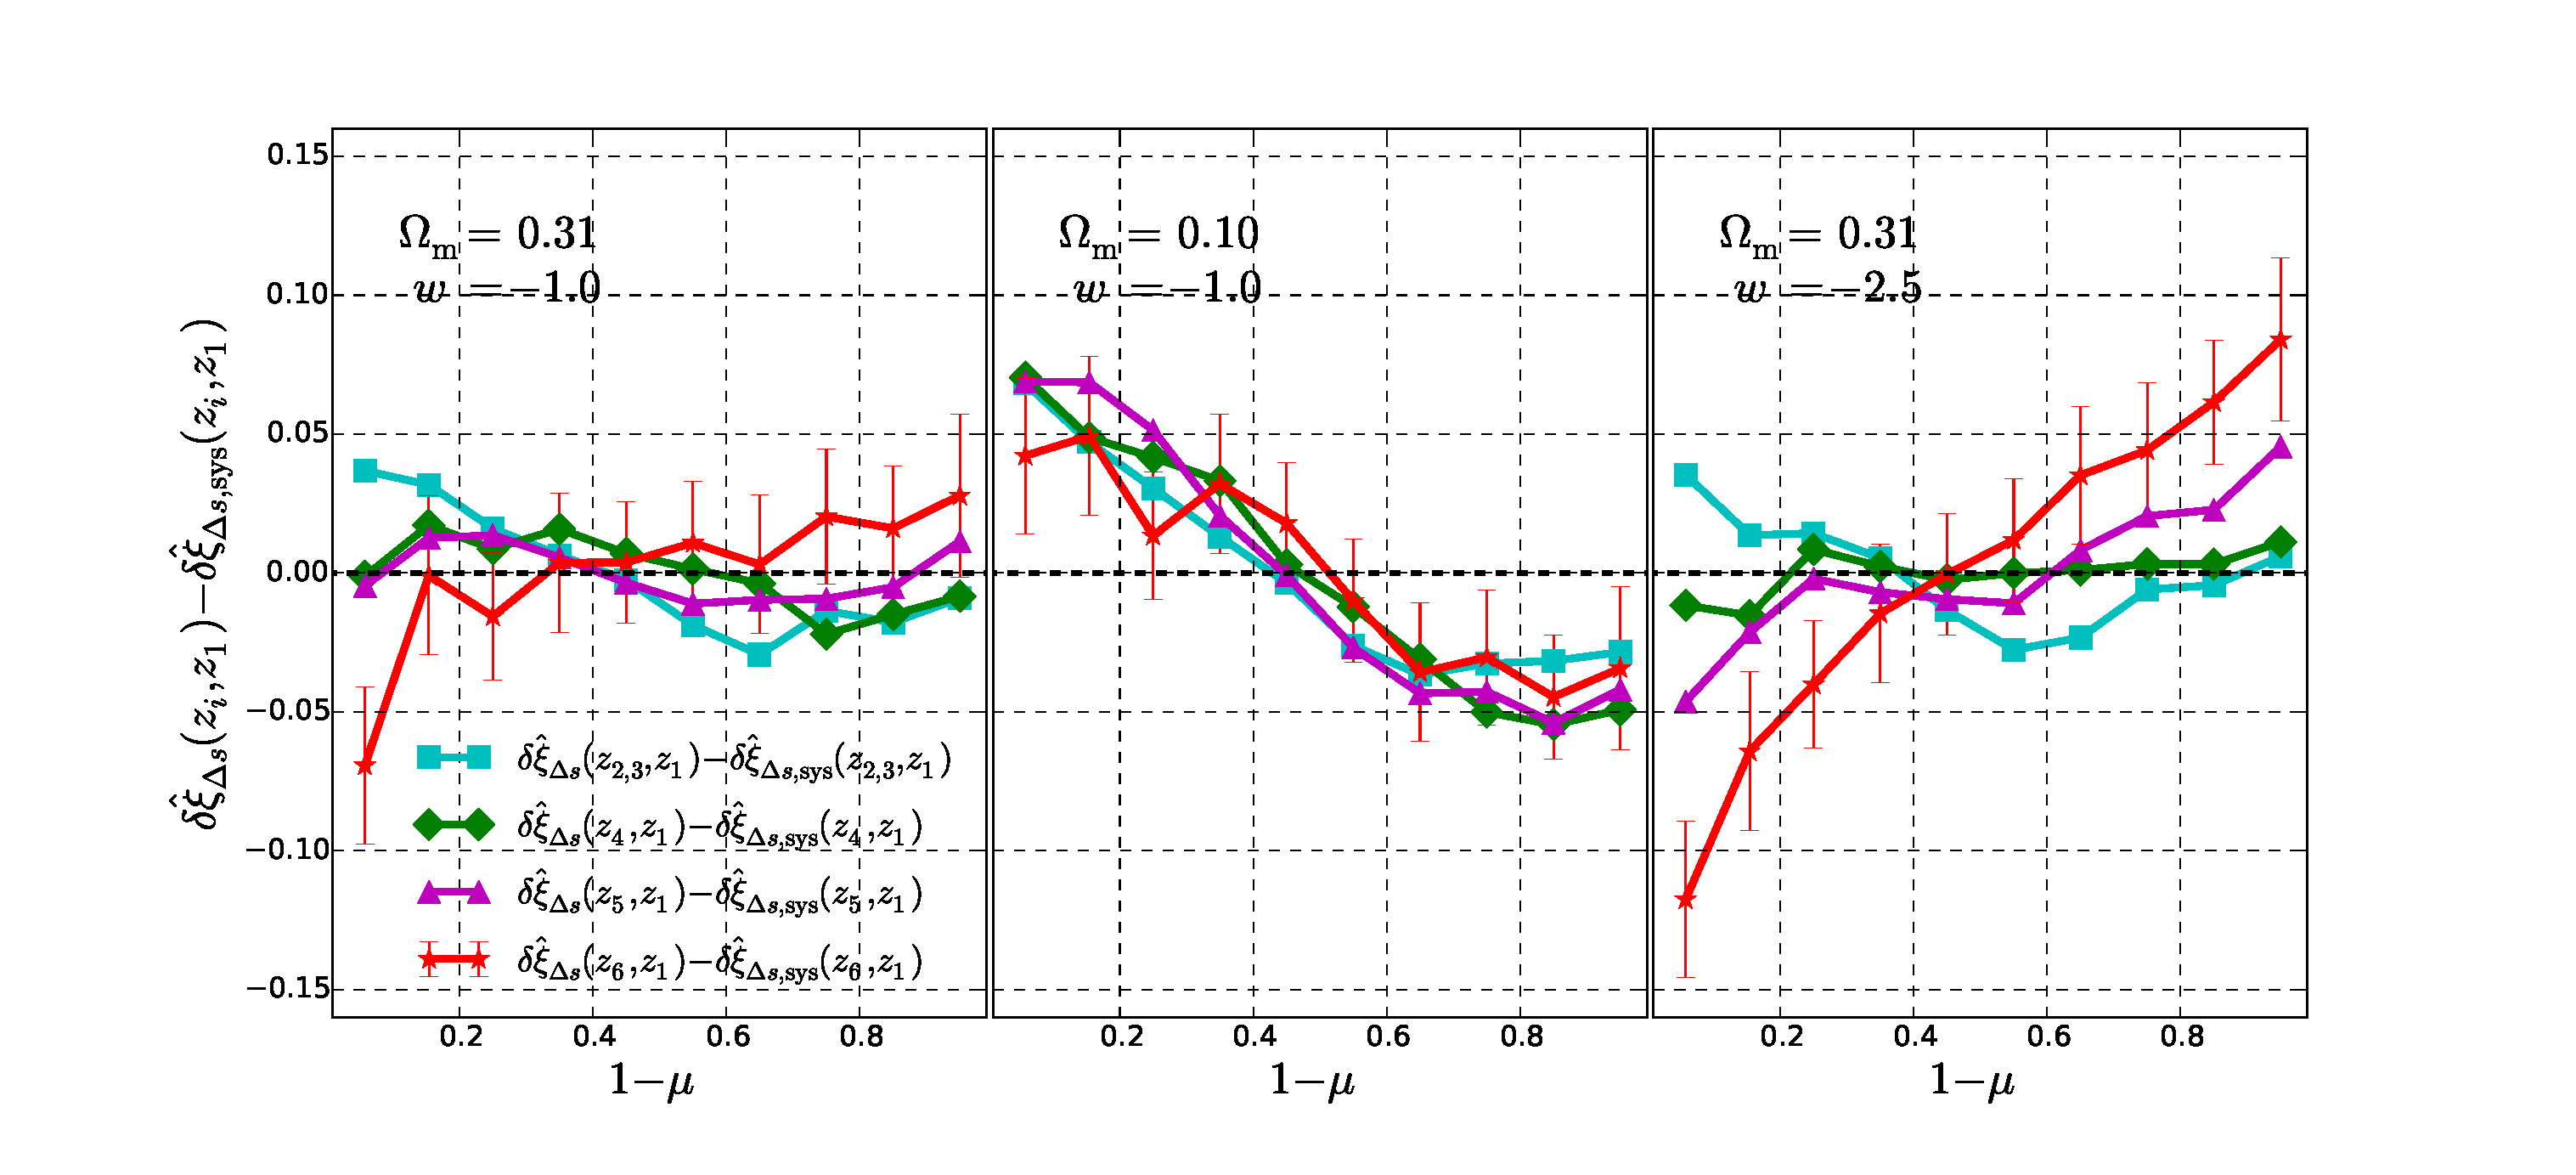
\includegraphics[width=18cm]{fig9_1.eps}
%   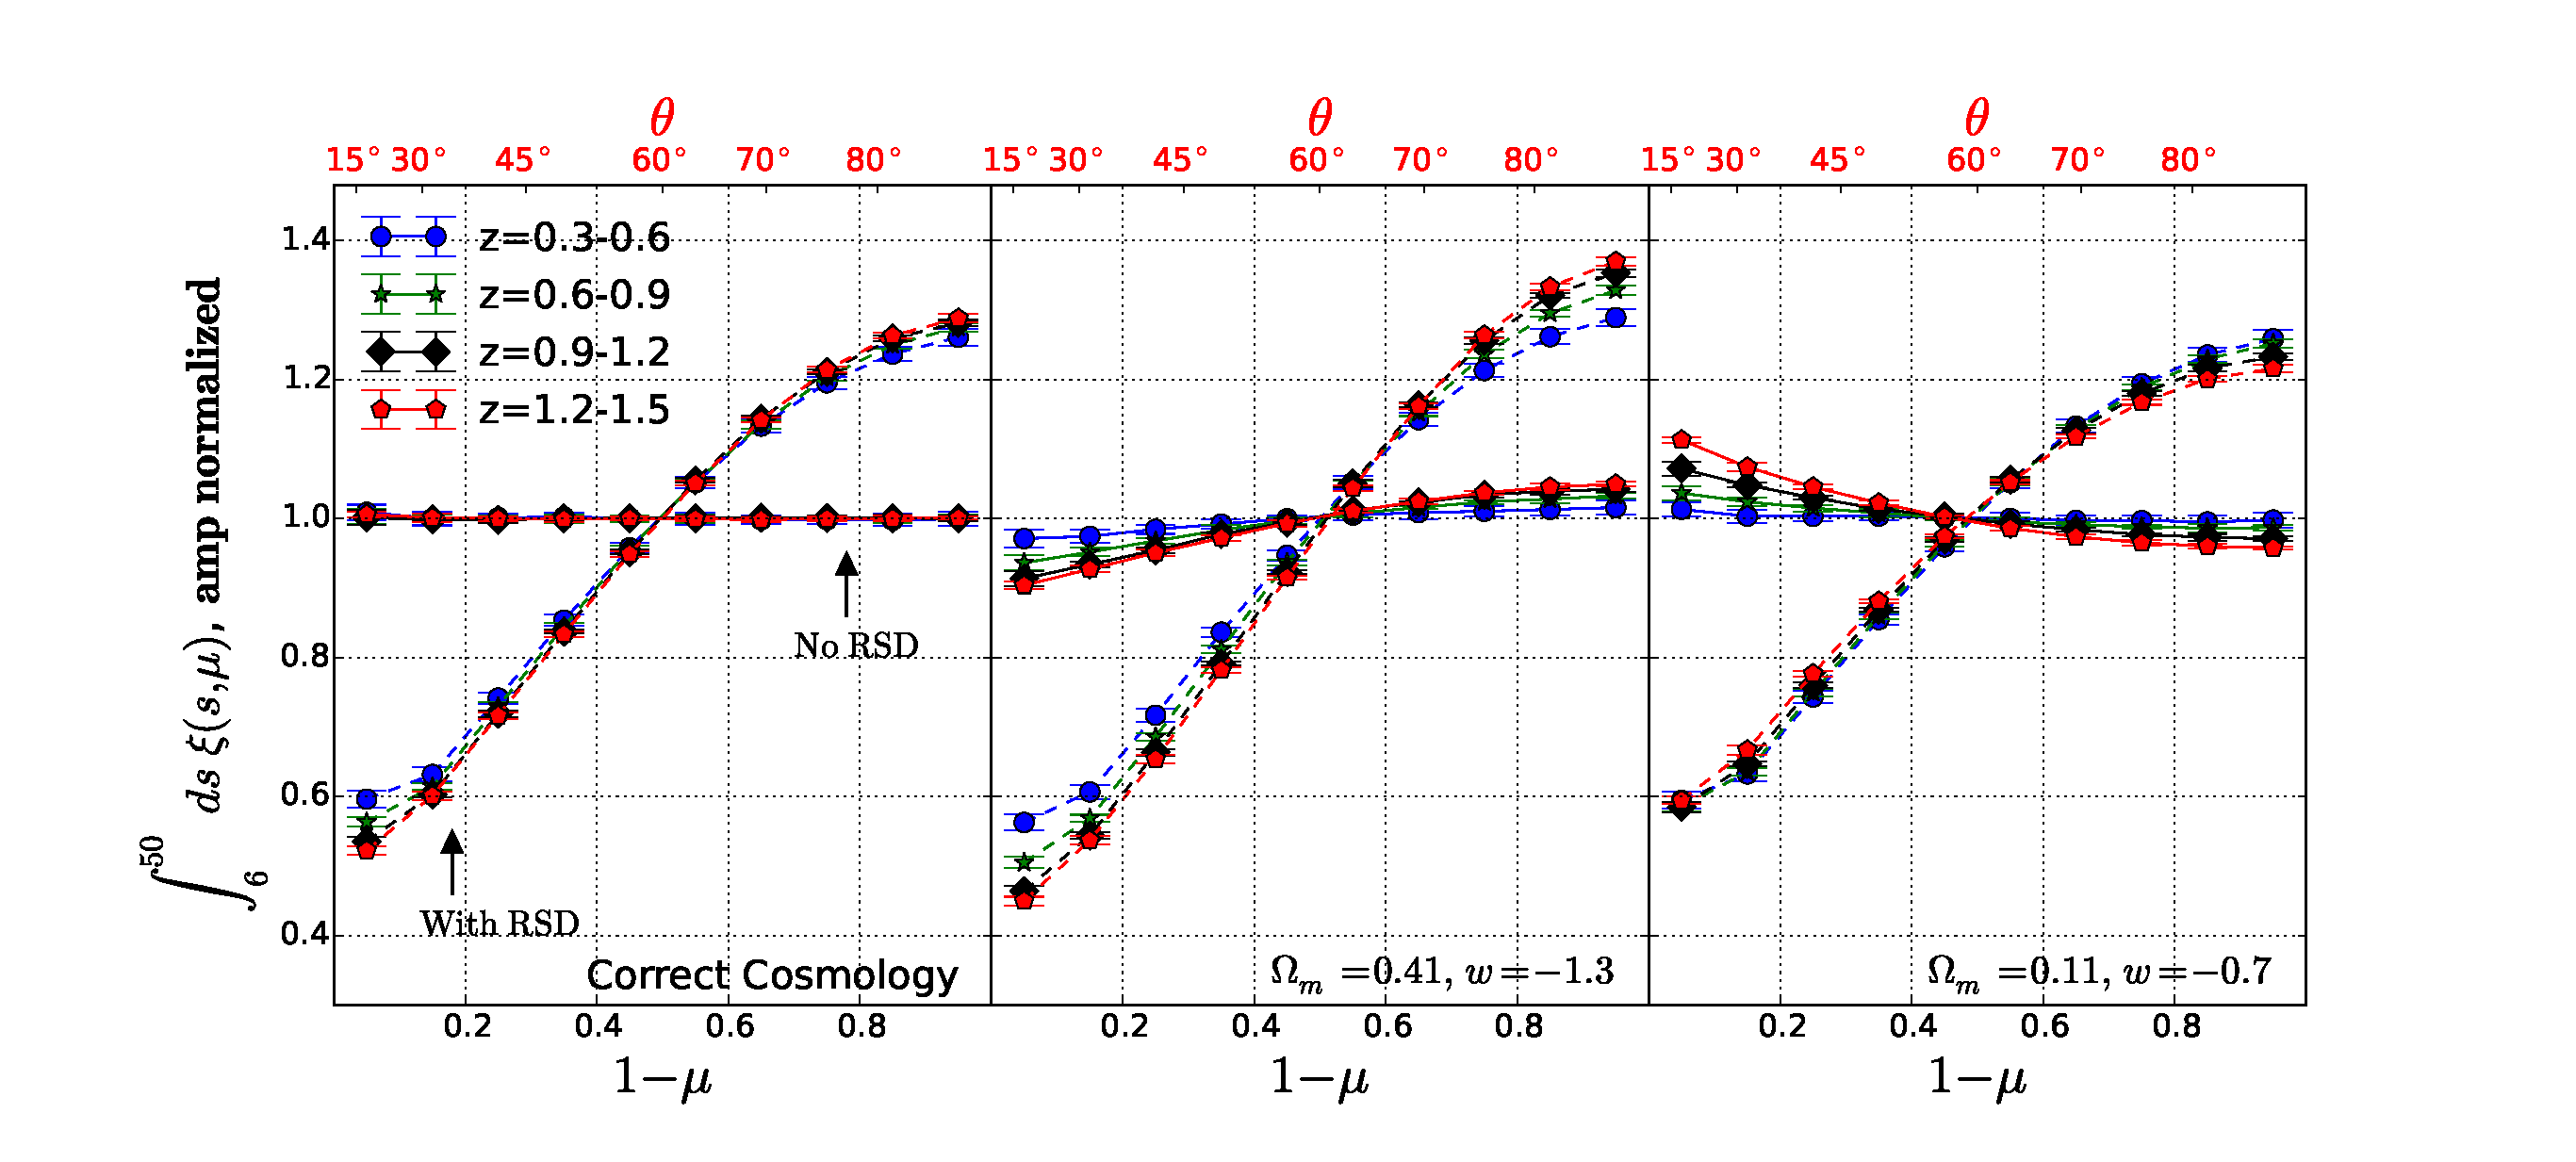
\includegraphics[height=8cm]{Tpcf--plot--Normed.eps}
%    \includegraphics[height=8cm]{smu.eps}
    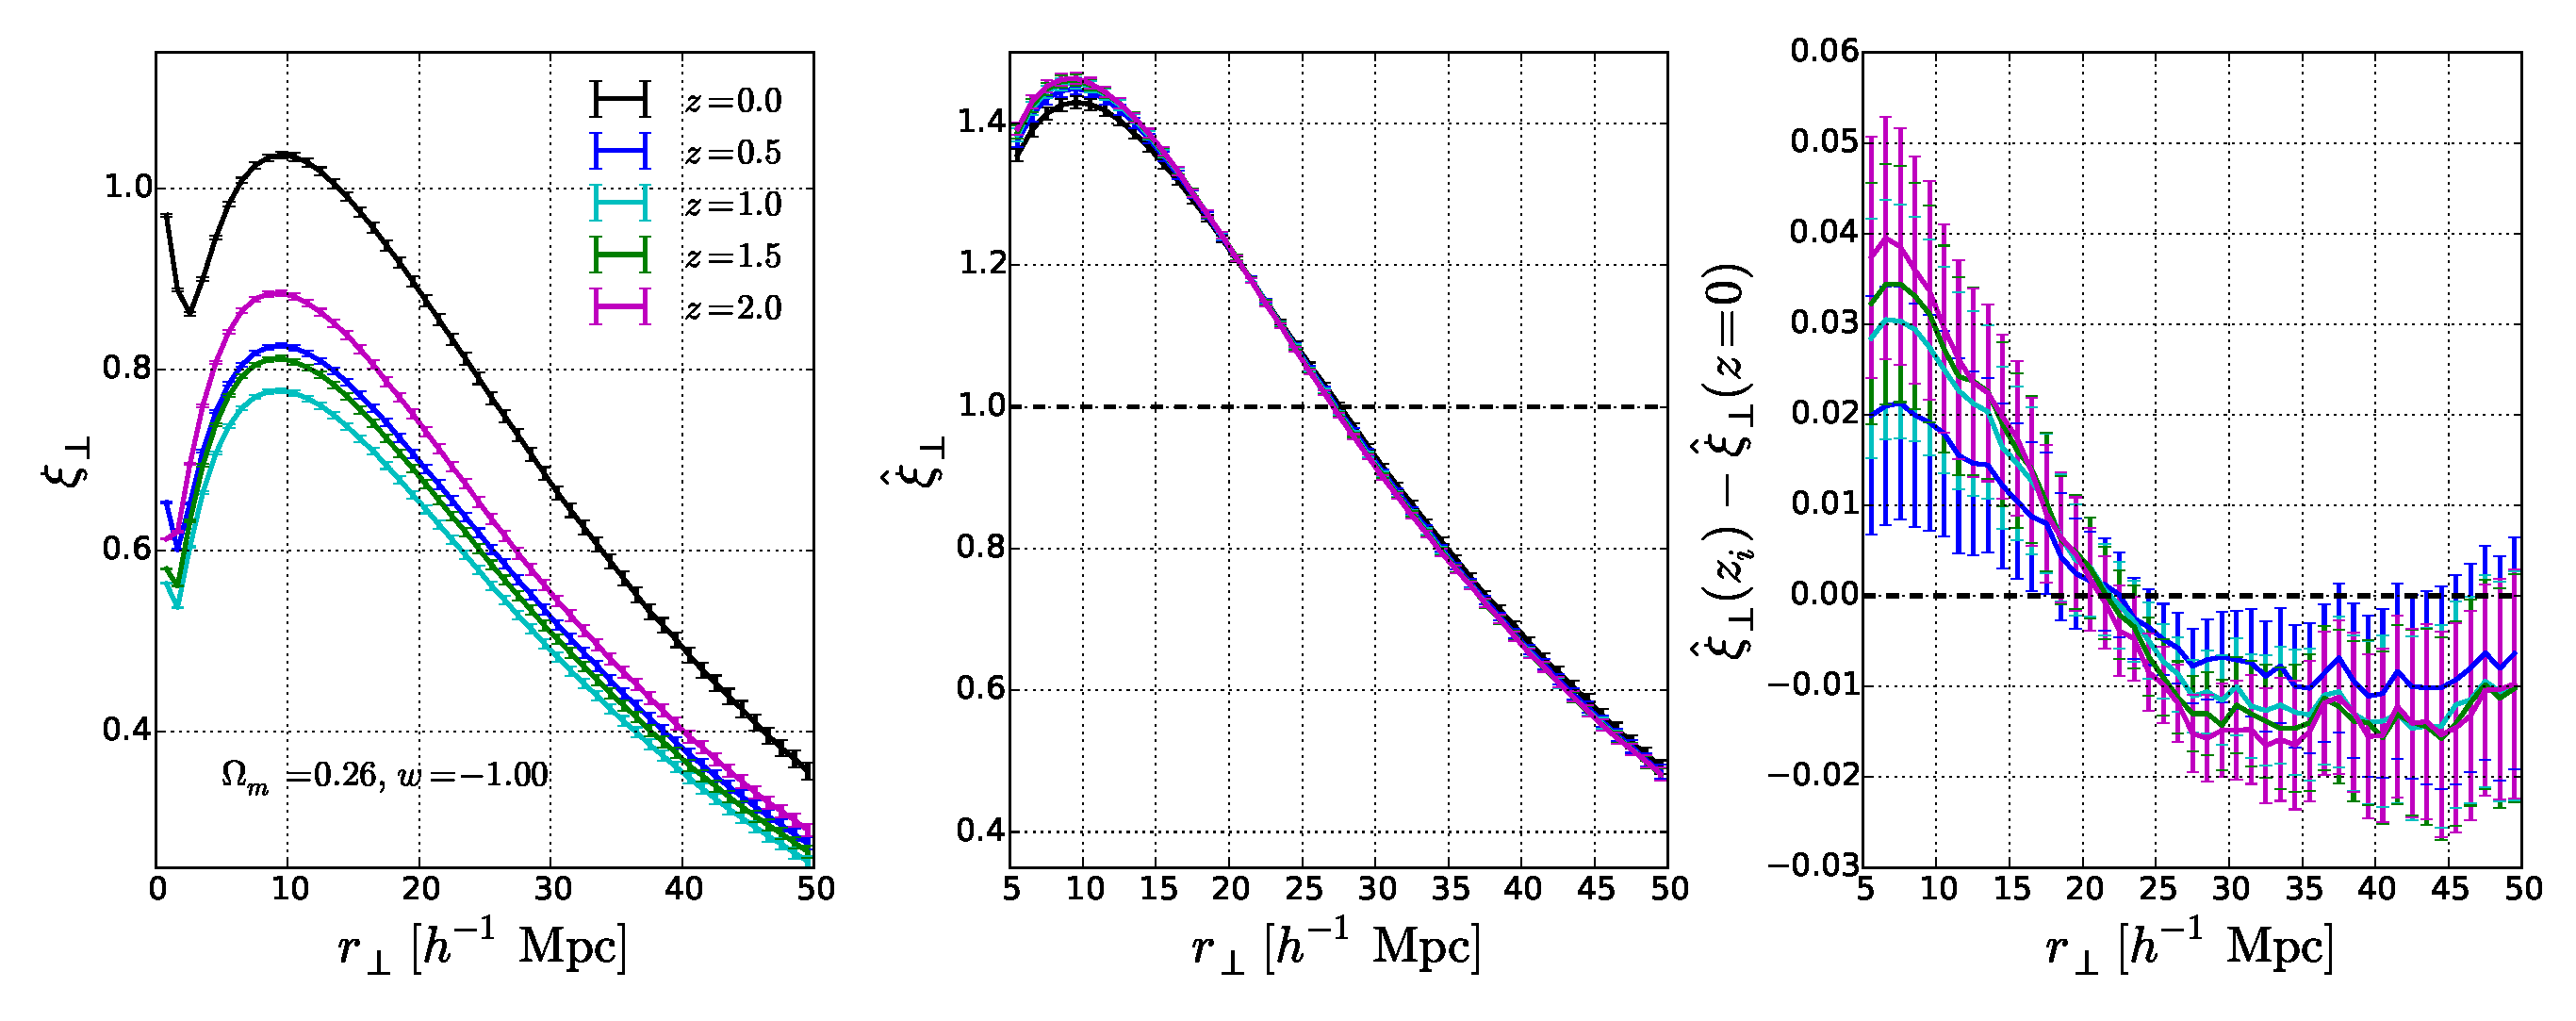
\includegraphics[width=18cm]{fig3.eps}
   }
   \caption{\label{fig_cosmo}
   2pCF in cosmologies.
   }
\end{figure*}


\begin{figure*}
   \centering{
   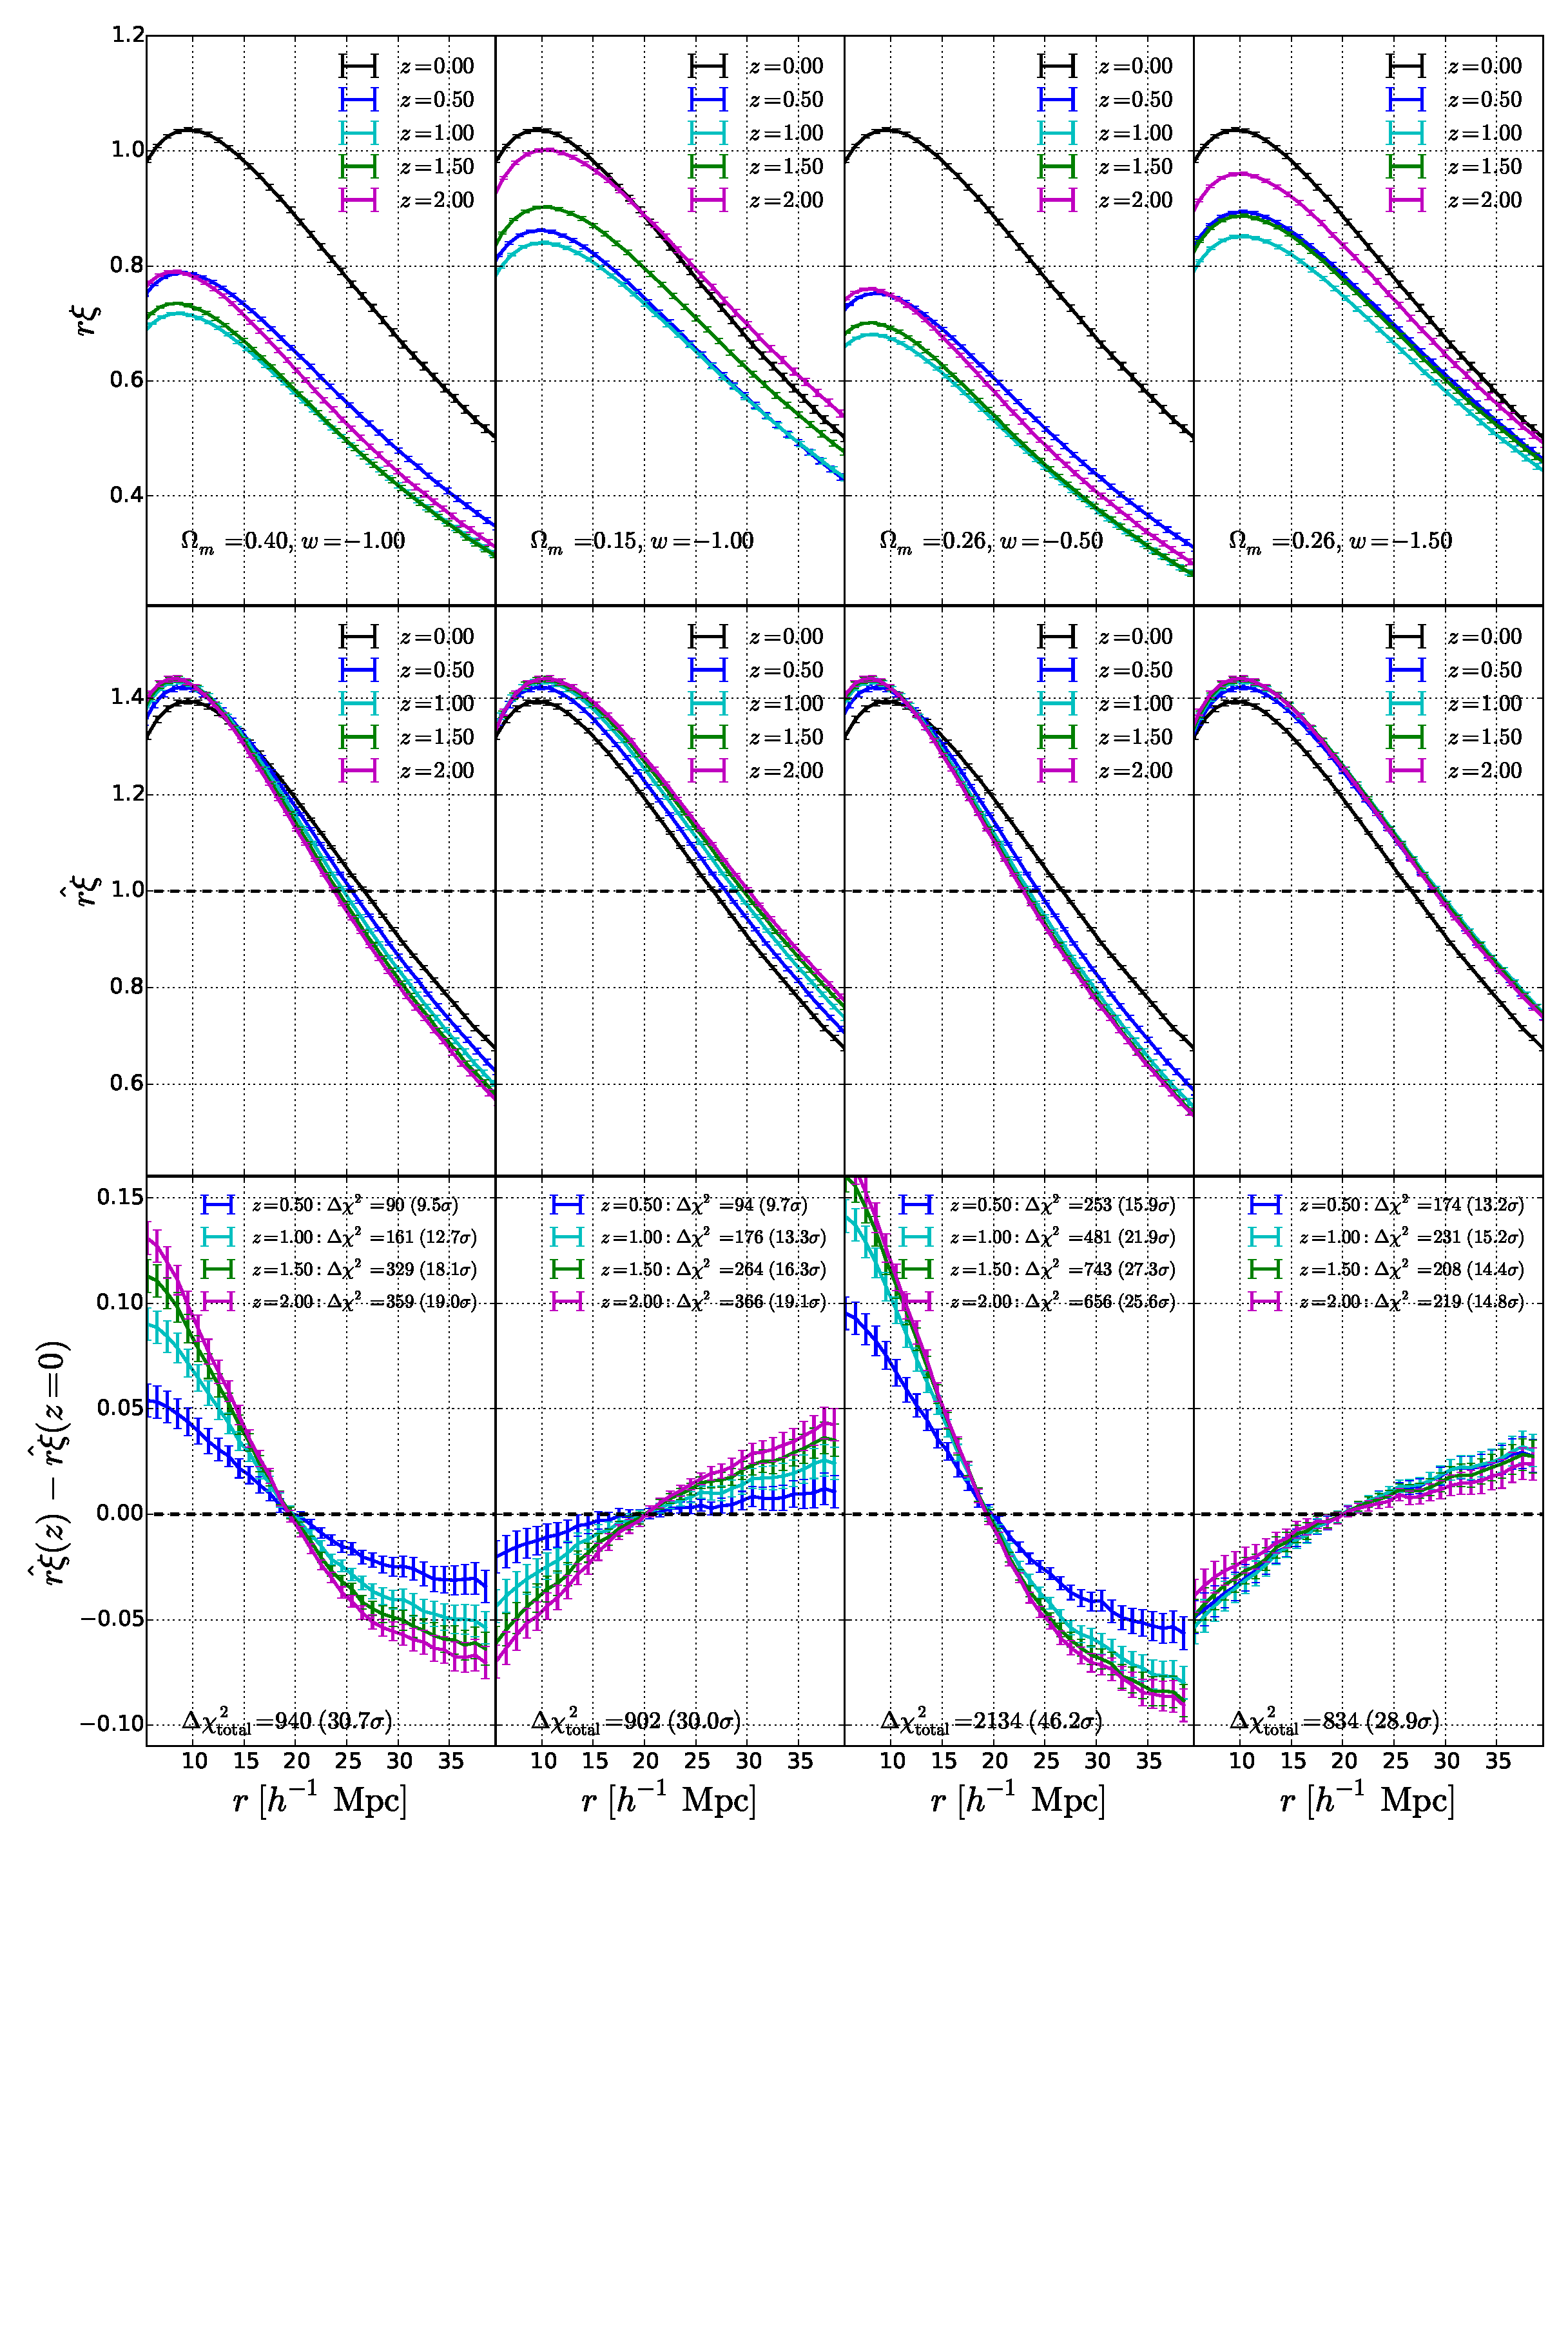
\includegraphics[width=16cm]{fig4.eps}
   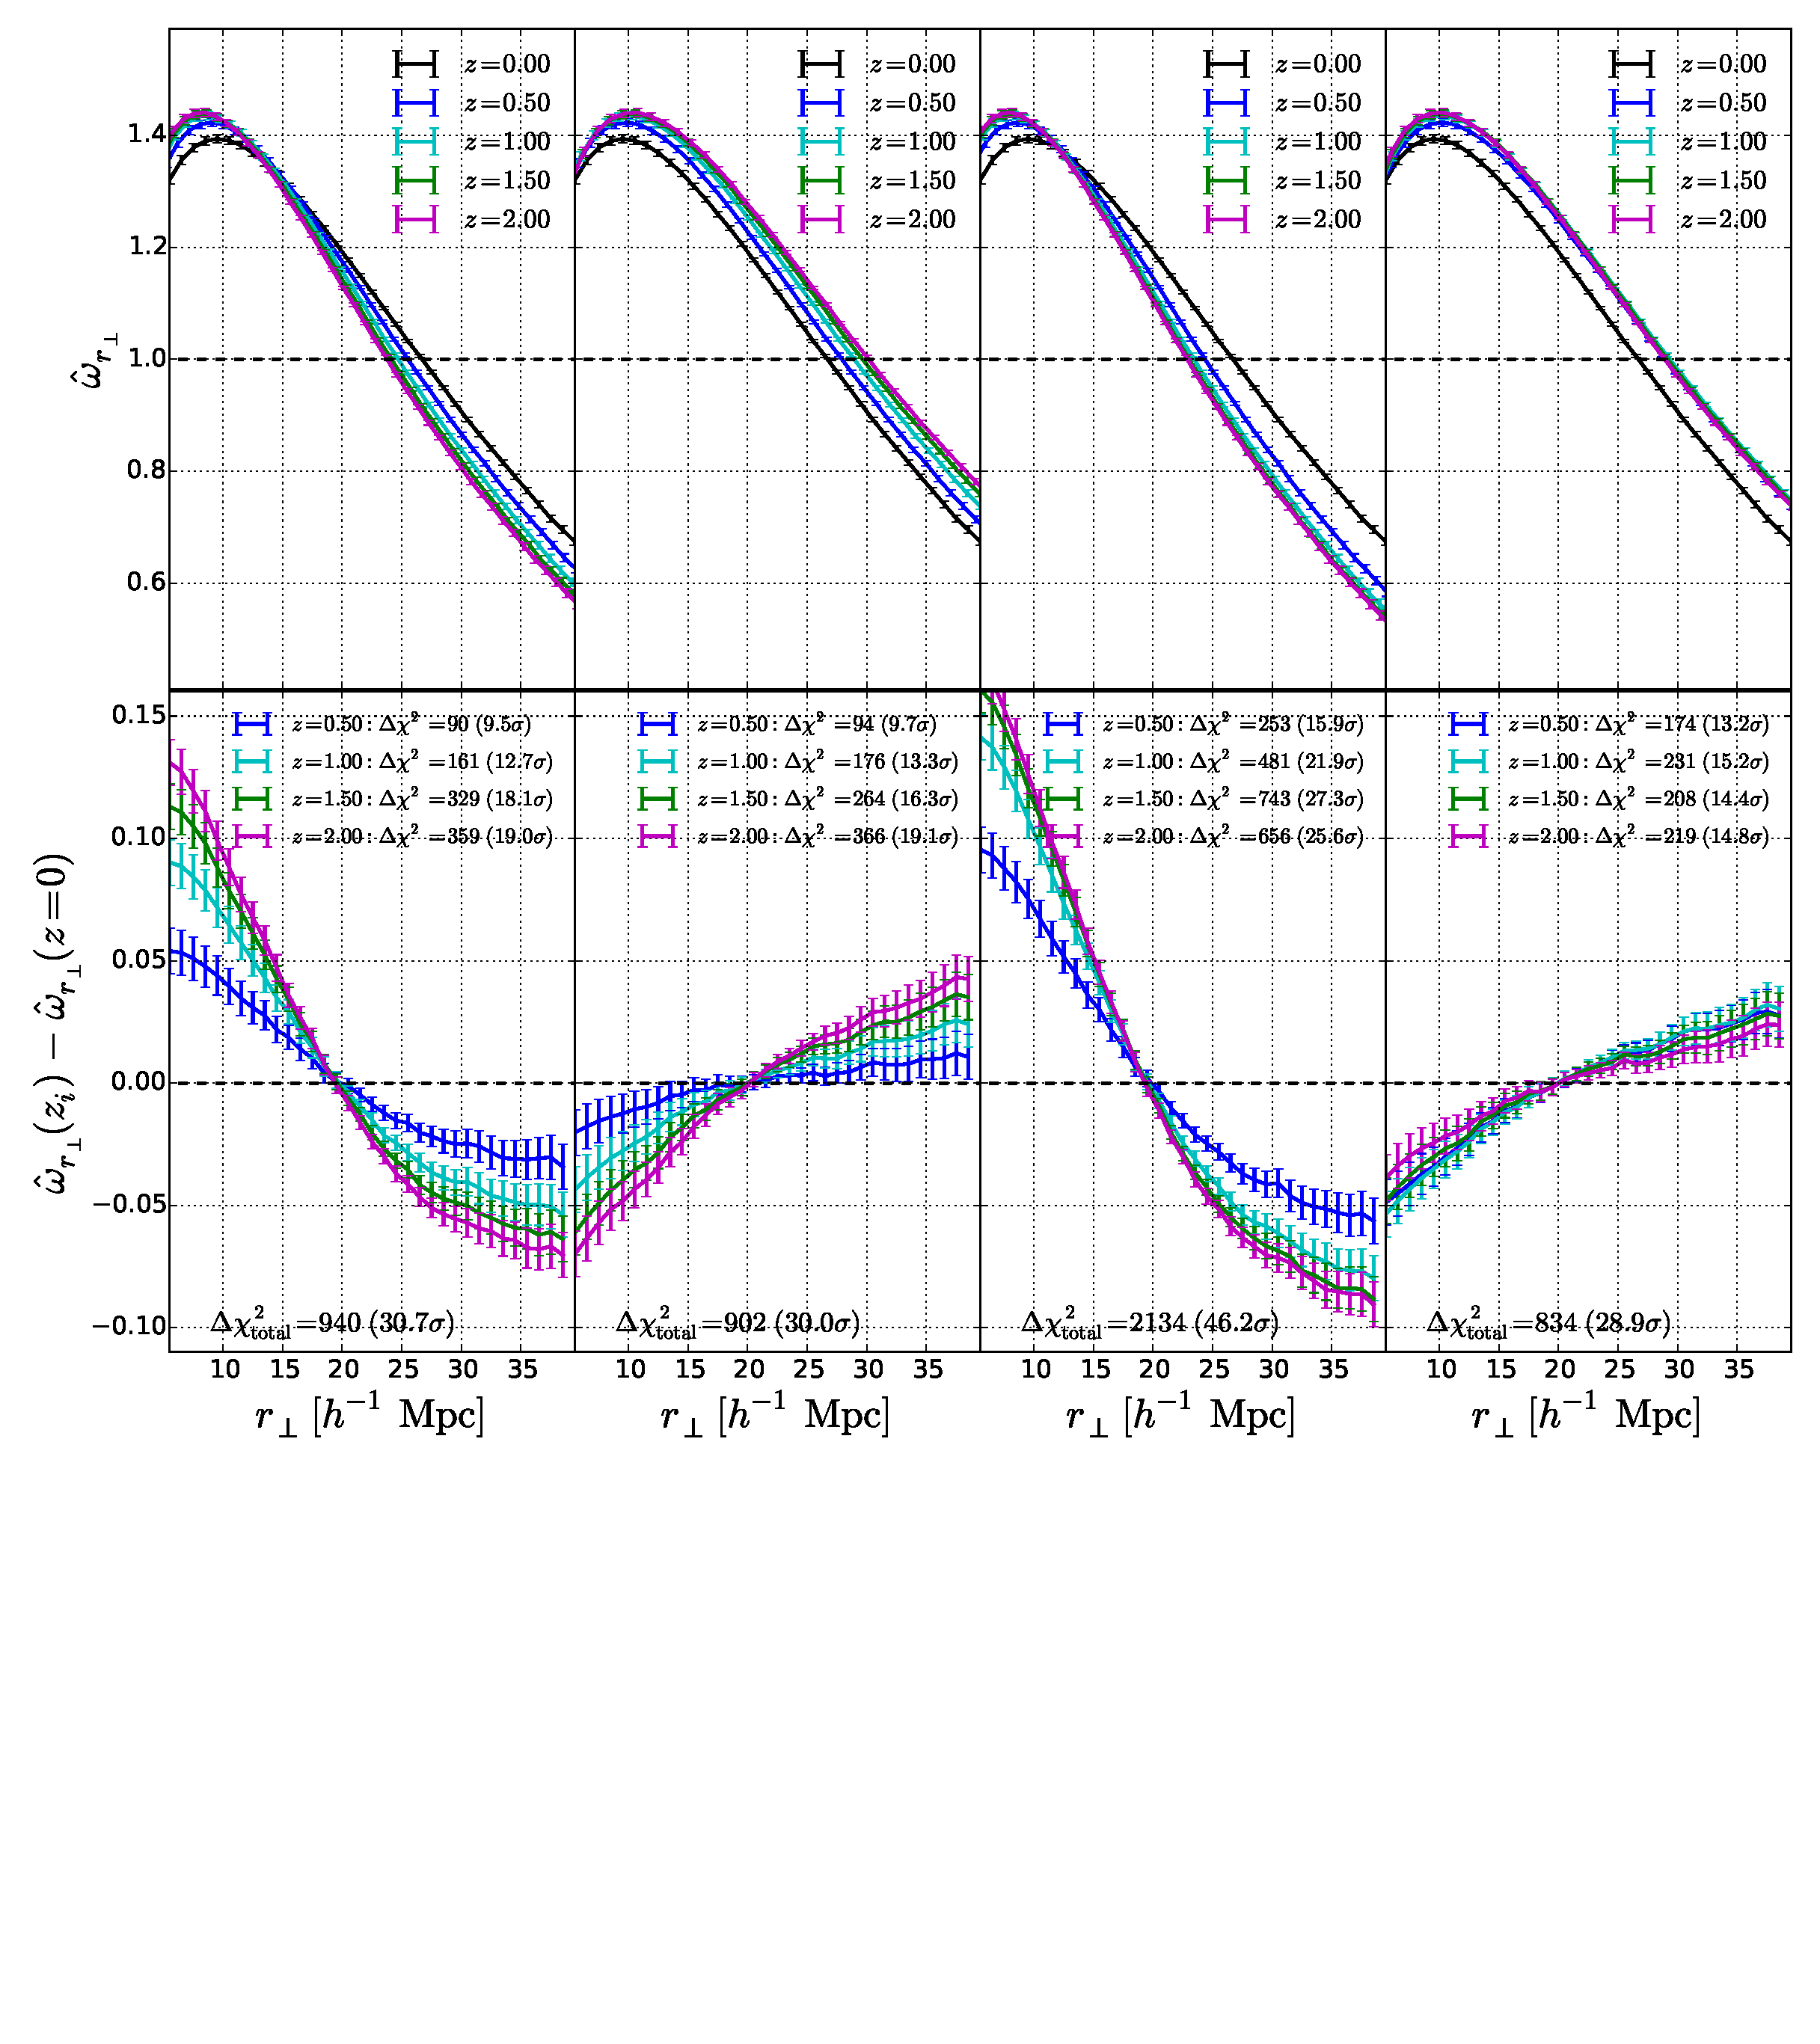
\includegraphics[width=16cm]{fig5.eps}
   }
   \caption{\label{fig_sys}
  Systematic effects.
   }
\end{figure*}


\section{cosmological constraint}



\section{Methodology}\label{sec:methodology}

We measure the angular 2pCF in the five redshifts.
We determine cosmological parameters by examining the redshift evolution of clustering anisotropy.
Mock survey samples are used to correct the results for the systematics and to estimate the covariance.
%Our procedure is as follows.

%\begin{minipage}{0.9\linewidth}
%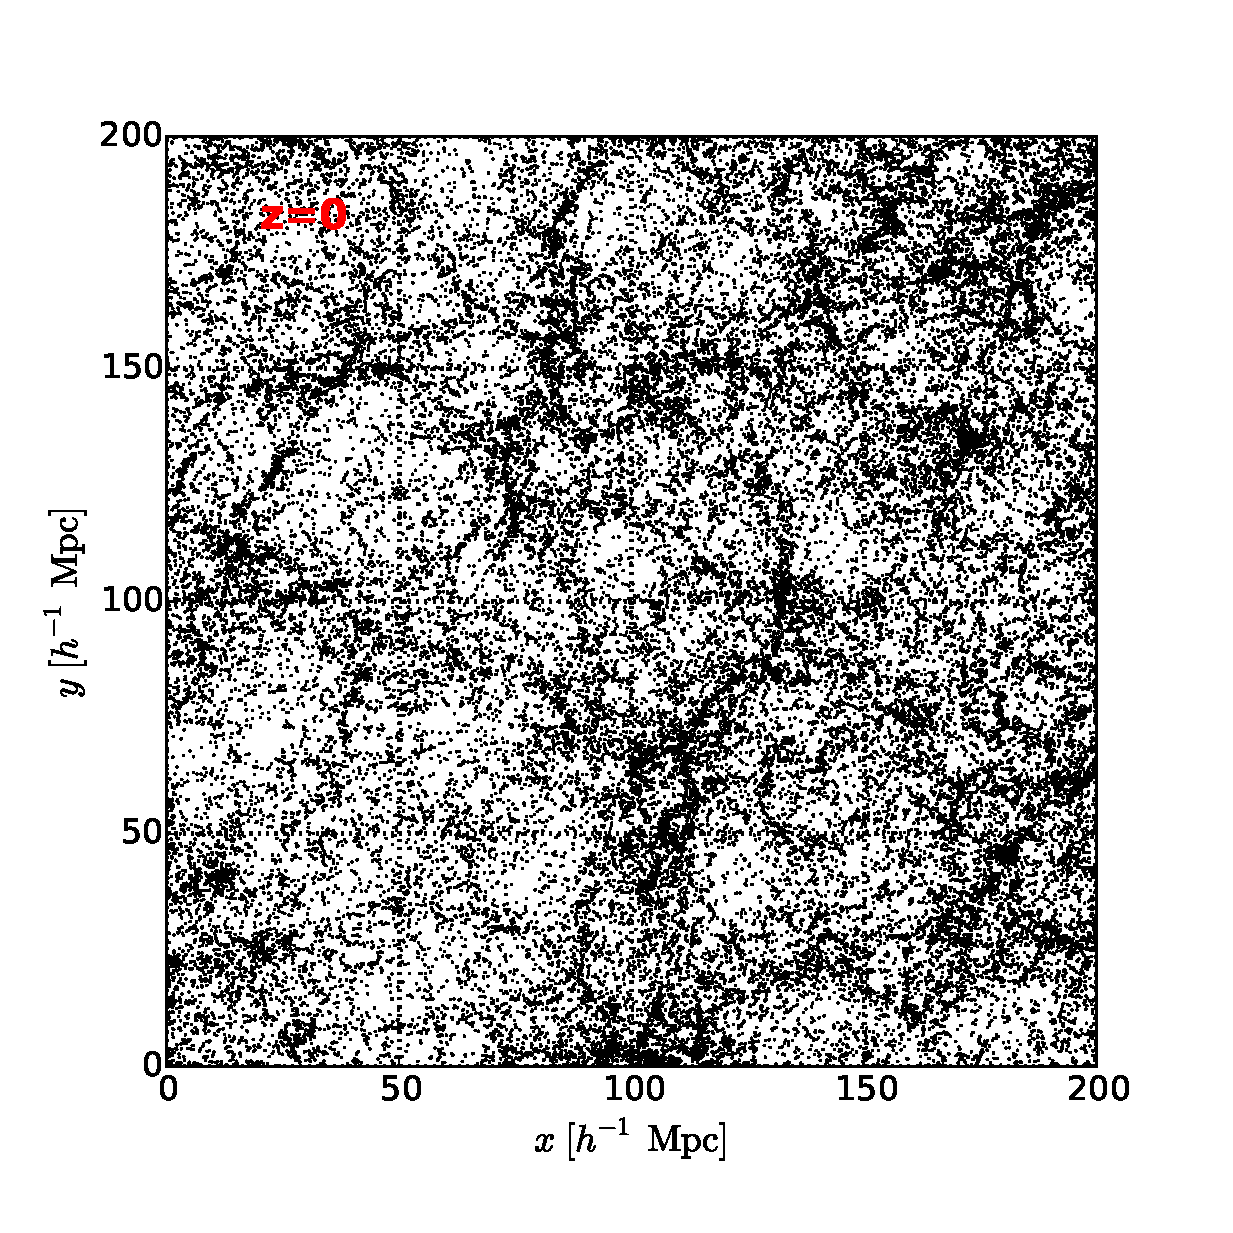
\includegraphics[width= 0.3\linewidth]{fig8_0.eps}
%\caption{\label{fig8} hahaha}
%\end{minipage}





\subsection{Grid of cosmology parameters}

The observed coordinates ({\it RA, Dec, z}) of galaxies
need to be converted to comoving coordinates ({\it x, y, z}) for the 2pCF analysis.
The dependence of clustering anisotropy on cosmology enters through the conversion from redshift to comoving distance,
i.e. the distance-redshift relation $r(z)$.
We consider the case of a flat Universe dominated by matter and dark energy,
so our $r(z)$ is governed by two parameters, $\Omega_m$ and $w$, as presented in Equation (\ref{eq:HDA})	.

To constrain these two parameters we examine the parameter space of 
$0.06\leq \Omega_m\leq 0.41$ and $-1.5 \leq w \leq -0.4$ with intervals of 
$\delta \Omega_m = 0.005$ and $\delta w = 0.025$,
forming a 71$\times$45 grid.
%This coverage and step size shall be enough for us to determine the 95\% confidence level (CL) region with satisfactory precision.
For each set of ($\Omega_m$, $w$), 
the comoving coordinates of all galaxies are computed, 
%the 2pCF of these galaxies in six redshift bins are measured,
%and a $\chi^2$ value is then obtained by requiring least redshift evolution of anisotropy.
%This enables us to infer the values and underlying distributions of $\Omega_m$ and $w$ through Bayesian analysis.
and the 2pCF is ready to be calculated.

\begin{figure*}
   \centering{
%   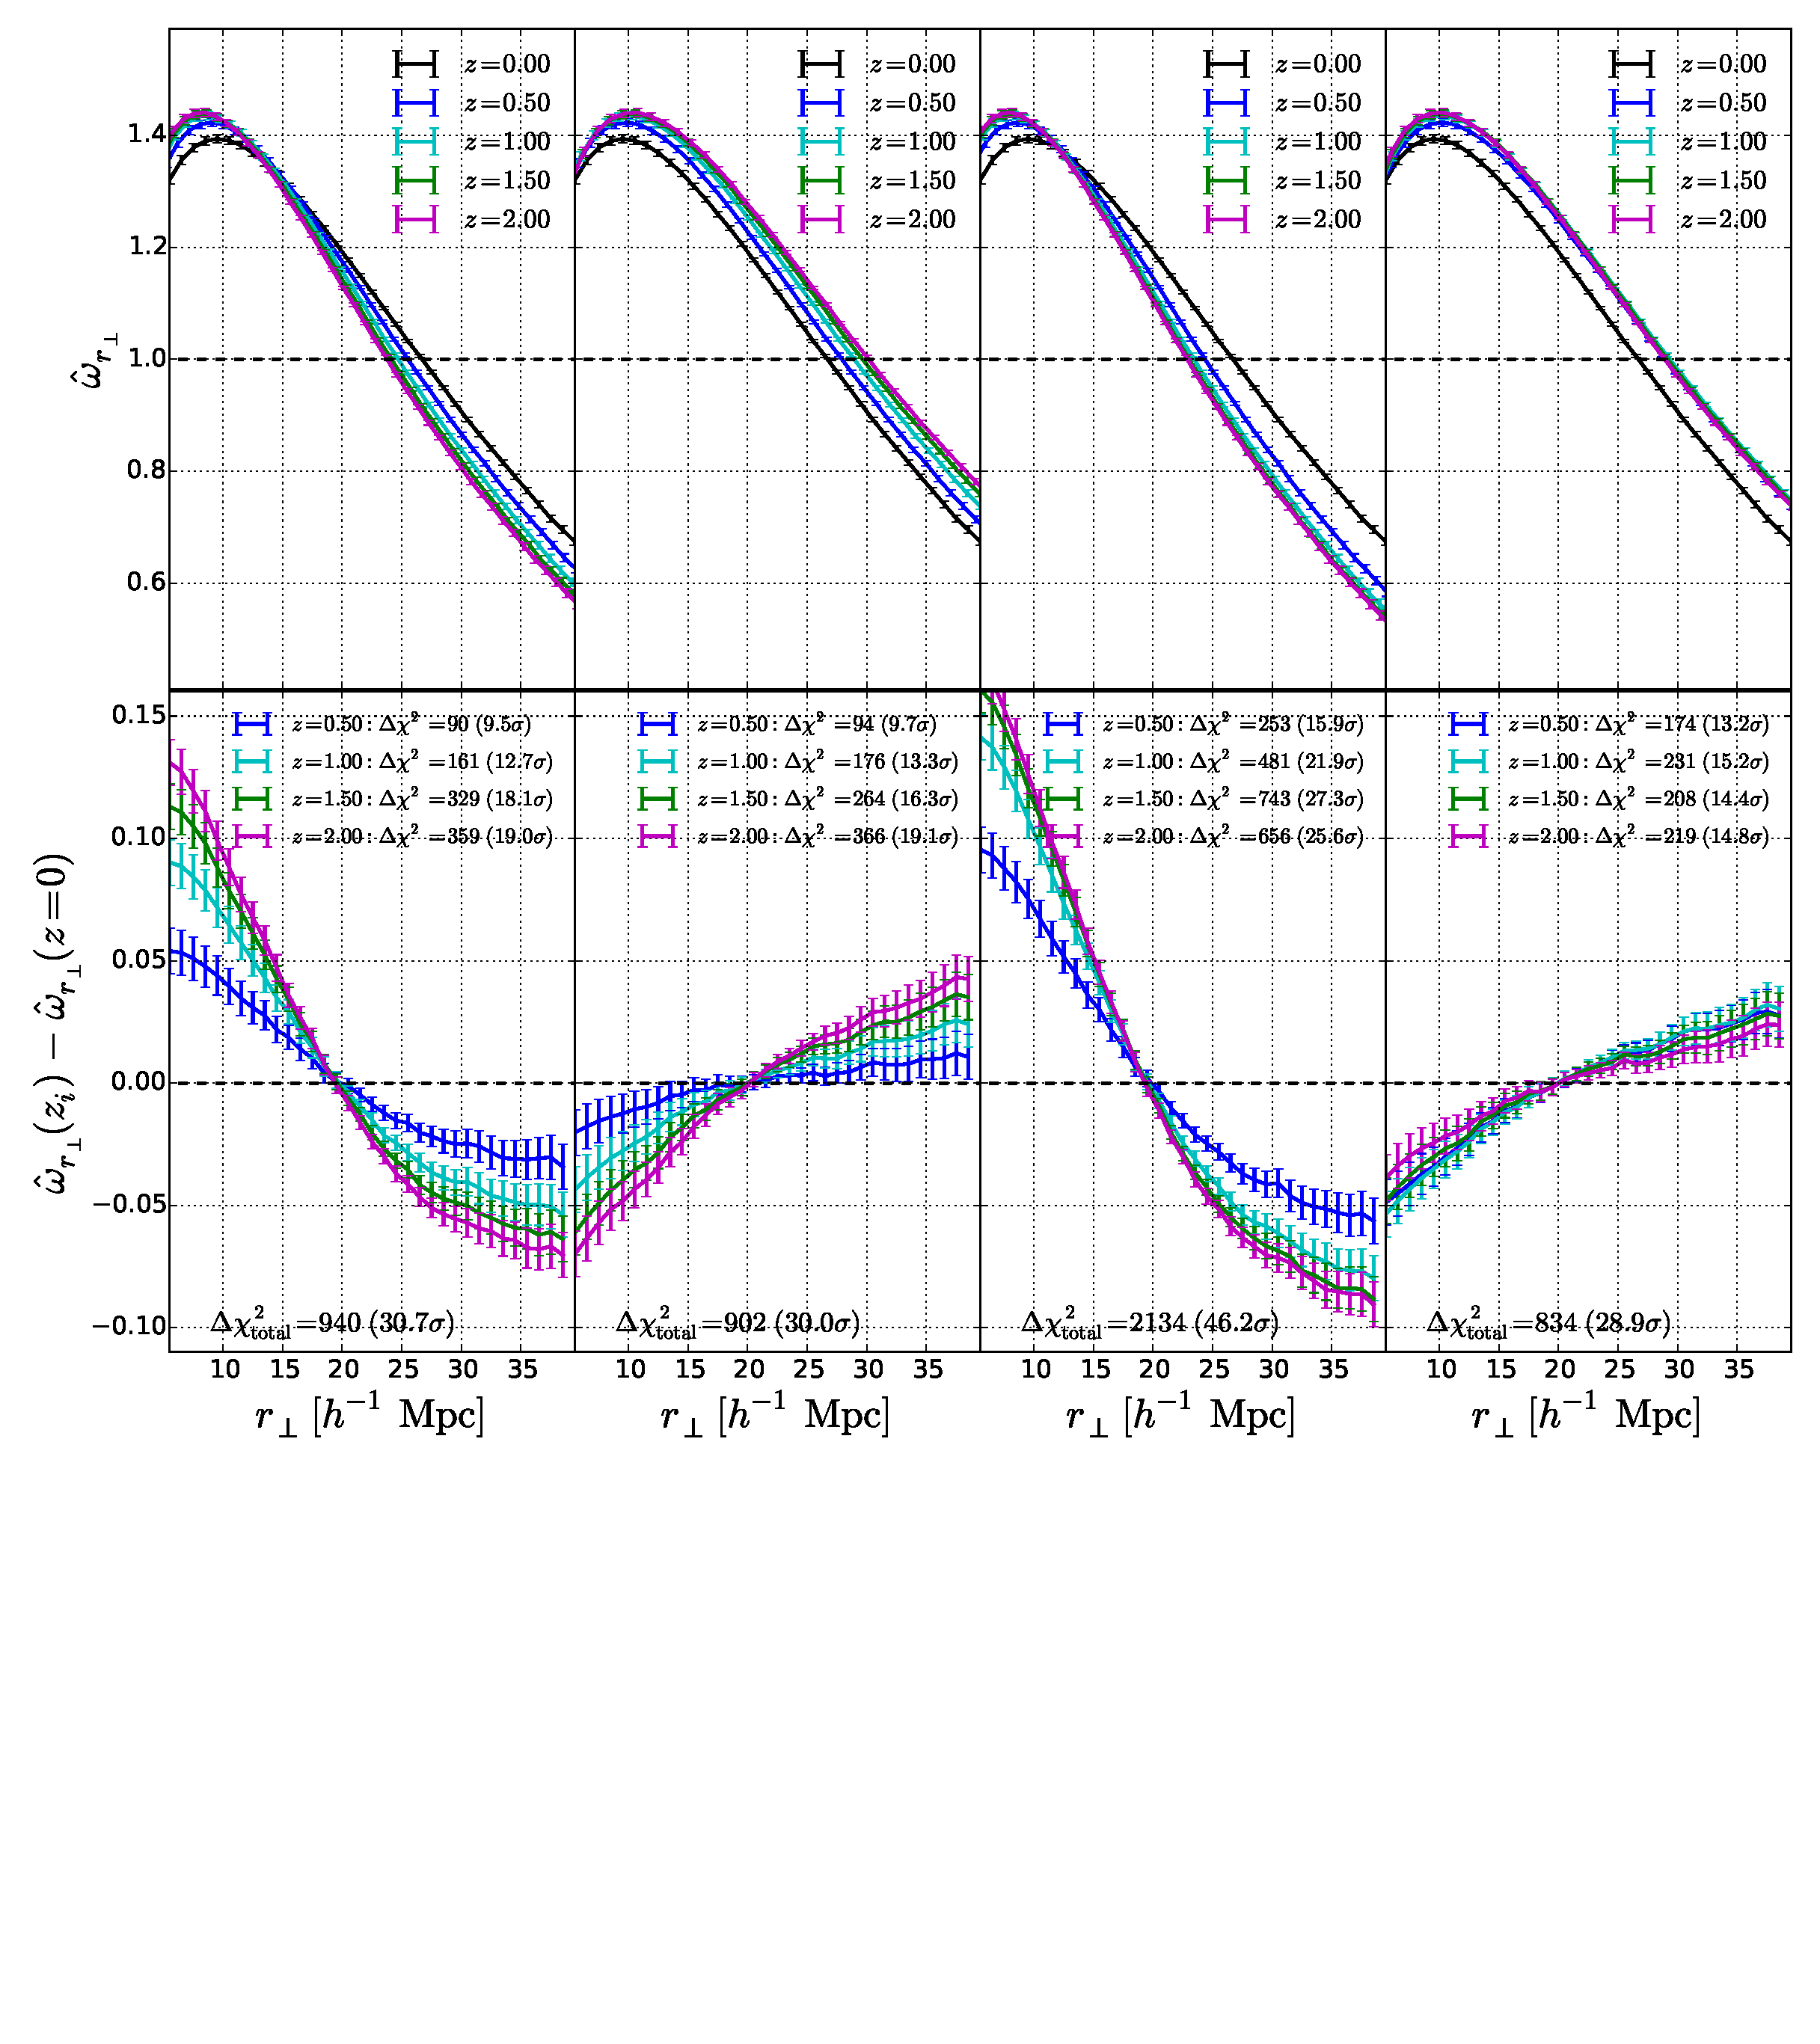
\includegraphics[width=14cm]{fig5.eps}
   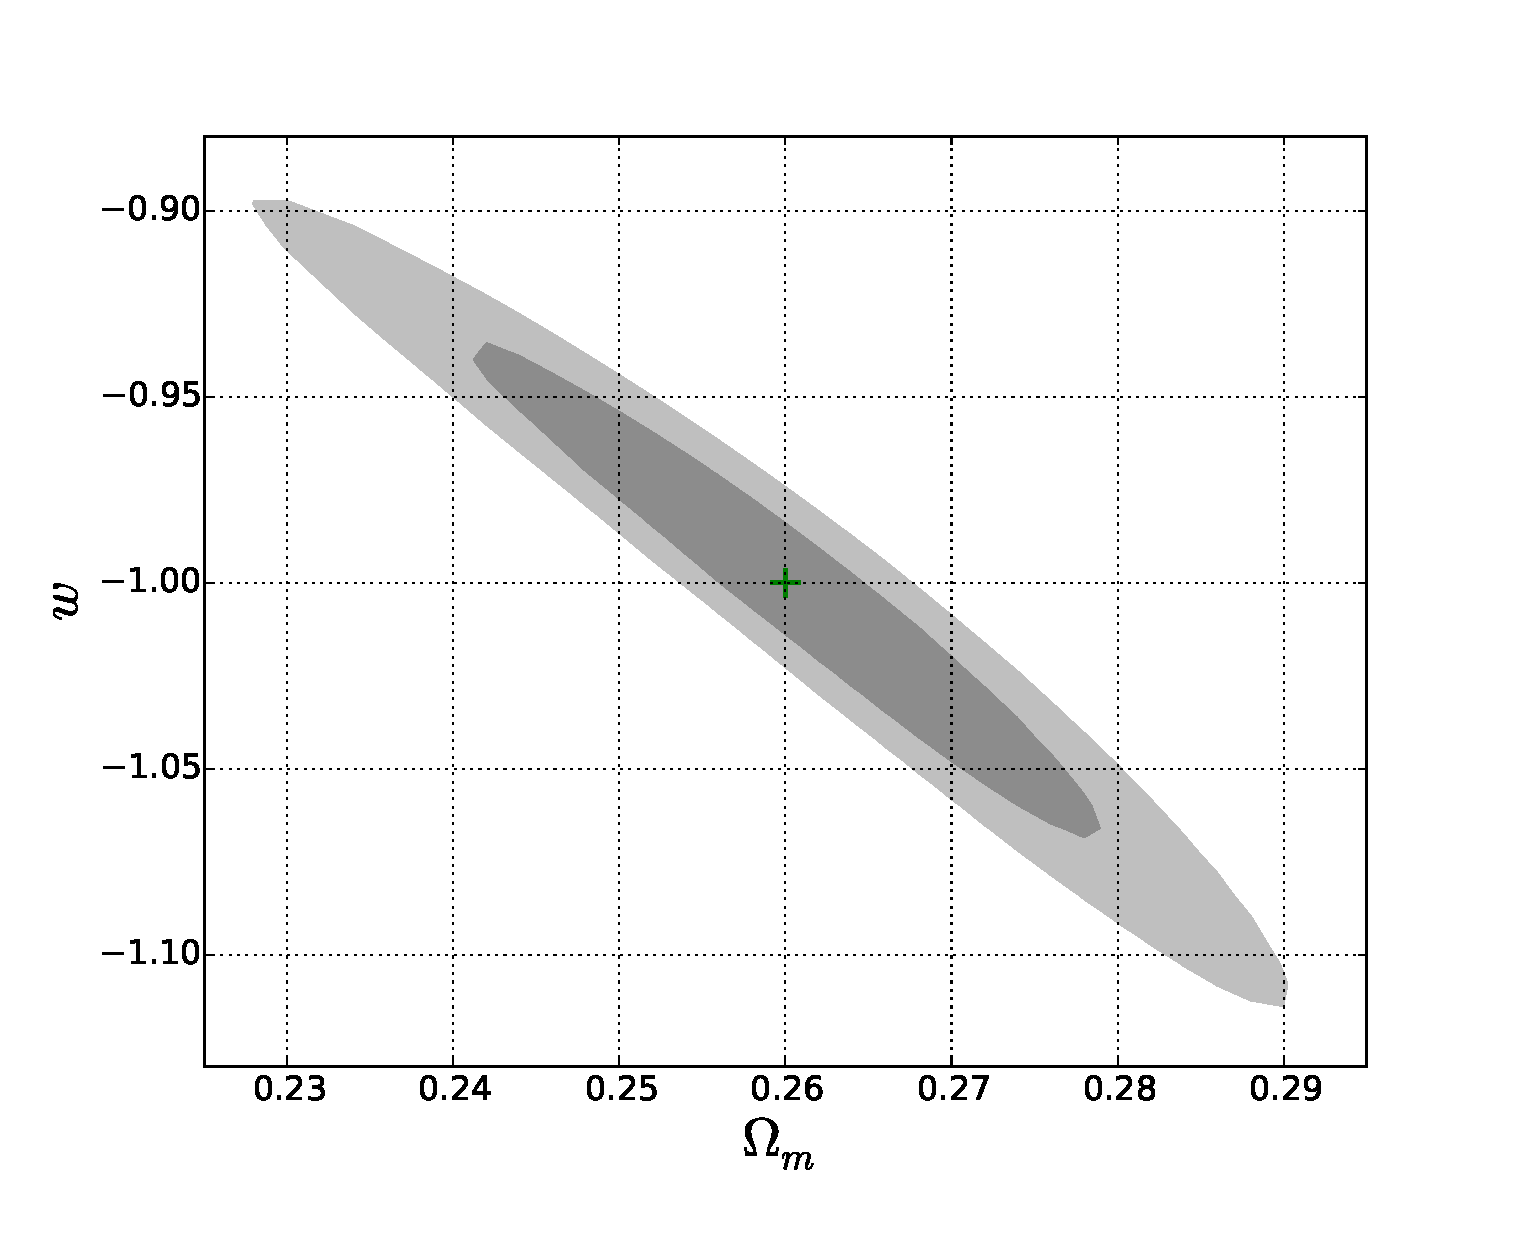
\includegraphics[width=14cm]{fig9.eps}
   }
   \caption{
    \label{fig_2pcfcon} 
    2D contour map of measured $\xi$ as a function of $\mu$ and $s$, from the six redshift bins of LOWZ and CMASS samples 
      in the cosmology of $\Omega_m=0.31$ $\Lambda$CDM model.
    The black dashed lines mark the scales 6\ $h^{-1}$Mpc $\leq s\leq$ 40\ $h^{-1}$Mpc.
    %The correlation functions have rather large values on small sales such as $s=5$ $h^{-1}$Mpc,
    %  and monotonically decreases to smaller values on larger scales due to weaker clustering.
    The contour lines are not horizontal due to the effects of peculiar velocity.
    The FOG and Kaiser effects clearly manifest themselves through the tilting of contour 
     lines where $1-\mu \rightarrow 0$ and $1-\mu \gtrsim0.1$, respectively.
    The six contour maps have rather similar appearance, implying small redshift evolution of $\xi$.
   }
      %The redshift density distribution of the BOSS DR12 galaxy samples, assuming a $\Lambda$CDM cosmology with $\Omega_m=0.31$.
      %The blue and green solid histograms show the distribution of LOWZ and CMASS galaxies respectively. 
      %The vertical dashed lines define the 6 redshift bins that are used to cut the samples.   }
\end{figure*}



\subsection{Measuring the correlation function}

%We probe the Alcock-Paczynski effects using the 2pCF. 
%The 2pCF is a mature statistic in cosmology and its optimal estimation considers minimal variance 
%while dealing with complicated masks and selection functions. 
%The most commonly adopted formulation is that of the 
We adopt the Landy-Szalay estimator~\citep{1993ApJ...412...64L} to calculate the 2pCF,
\begin{equation}
\xi(s,\mu)=\frac{DD-2DR+RR}{RR}\ ,
\end{equation}
where $DD$ is the number of galaxy--galaxy pairs, 
$DR$ the number of galaxy-random pairs, 
and $RR$ is the number of random--random pairs, 
all separated by a distance defined by $s\pm\Delta s$ and $\mu\pm\Delta\mu$, 
where $s$ is the distance between the pair and $\mu=\cos(\theta)$, 
with $\theta$ being the angle between the line joining the pair of galaxies and the LOS direction to the target galaxy. 
This statistic captures the anisotropy of the clustering signal.

The random catalogue consists of unclustered points whose number density in redshift space mimics the radial selection function of the observational data. 
To reduce the statistical variance of the estimator we use 50 times as many random points as we have galaxies.
The galaxies and random points are weighted as described in Sec. \ref{sec:data}.

Figure \ref{fig_2pcfcon} shows the 2D contour of measured $\xi$ as a function of $\mu$ and $s$,
from the six redshift bins of LOWZ and CMASS samples 
in the cosmology of $\Omega_m=0.31$ $\Lambda$CDM model.
%The correlation functions have rather large values on small sales such as $s=5$ $h^{-1}$Mpc,
%and monotonically decrease to smaller values on larger scales due to weaker clustering.
Due to the peculiar velocity effect, the contour lines are not horizontal.
The FOG \citep{FOG} and Kaiser \citep{Kaiser1987} effects 
clearly manifest themselves through the tilting of contour lines in regions of $\mu \rightarrow 1$ and $1-\mu \gtrsim0.1$, respectively.
A visual inspection of the contour maps from the six redshift bins 
reveals that they all have a similar appearance,
implying small redshift evolution of $\xi$.

\subsection{Probing the anisotropy through 2pCF}

The 2pCF is measured as a function of the separation $s$ and the angular direction $\mu$.
To probe the anisotropy we are more interested in the dependence of the 2pCF on $\mu$.
We follow the procedure of \cite{Li2015} and integrate the $\xi$ over the interval $s_{\rm max} \leq s \leq s_{\rm min}$.
We evaluate
\begin{equation}\label{eq:xideltas}
\xi_{\Delta s} (\mu) \equiv \int_{s_{\rm min}}^{s_{\rm max}} \xi (s,\mu)\ ds.%,\ \ \ {\rm at\ particular\ binned\ direction\ }\mu_i
\end{equation}
The integration is limited at both small and large scales.
At small scales the value of $\xi$ is seriously affected by the FOG effect \citep{FOG}
which depends on the galaxies bias.
This may introduce a redshift evolution in $\xi_{\Delta s}(\mu)$ that is relatively difficult to model.
At large scales the measurement is dominated by noise due to poor statistics.
\cite{Li2015} found that $s_{\rm min}=6-10$ $h^{-1}$Mpc and $s_{\rm max}=40-70$ $h^{-1}$Mpc are reasonable choices 
which provide consistent, tight and unbiased constraints on cosmological parameters.
In this analysis we choose $s_{\rm min}=6$ $h^{-1}$Mpc and $s_{\rm max}=40$ $h^{-1}$Mpc.

The redshift evolution of the bias of observed galaxies leads to redshift evolution of the strength of clustering,
which is difficult to accurately model.
To mitigate this systematic uncertainty we rely on the shape of $\xi_{\Delta s}(\mu)$, rather than its amplitude,
\begin{equation}\label{eq:norm}
 \hat\xi_{\Delta s}(\mu) \equiv \frac{\xi_{\Delta s}(\mu)}{\int_{0}^{\mu_{\rm max}}\xi_{\Delta s}(\mu)\ d\mu}.
\end{equation}
We impose a cut $\mu<\mu_{\rm max}$ to reduce the fiber collision and FOG effects which are stronger toward the LOS ($\mu\rightarrow1$) direction.



The clustering properties may be affected by various properties of the galaxy sample, 
such as, for example the mass, morphology, color, concentration. 
In our simulation, using the merger tree, 
we identify ``galaxies'', therefore we only use the galaxy mass building history to simulate BOSS galaxies. 
Therefore, it is necessary for us to test if our mock galaxies can accurately 
reproduce the $\hat\xi_{\Delta s}(\mu)$ of observed galaxies.

%The clustering properties may be affected by the redshift evolution of properties of the galaxy sample, 
%such as the mass, morphology, color, concentration, and so on. 
%In our simulation, using the merger tree, we identify 'galaxies' so that we only use the galaxy mass to simulate BOSS galaxies. Therefore, it was necessary for us to test if our mock galaxies can accurately reproduce the shape of $\xi_{\Delta s}(\mu)$ of observed galaxies.

%As shown by Figure 6, the mock galaxies from our HR4 simulation can well reproduce the 
%$\hat\xi_{\Delta s}(\mu)$ of the observed galaxies.
Figure \ref{fig_datamock}  compares the shape of $\hat\xi_{\Delta s}(\mu)$ measured from observational data and mock survey samples.
It is clear that $\hat \xi_{\Delta s}(\mu)$ from mock galaxies identified in the HR4 simulation (green dotted line) agrees well with the observation.
%The HR4 galaxy mock can well reproduce the result from observational measurement.
The enhancement near $\theta=0^\circ$ is caused by the FOG effect,
and the characteristic shape in $20^\circ\lesssim\theta\lesssim90^\circ$ 
produced from the large-scale flow
are all very well reproduced.
This result verifies the ability of our mock galaxies to reproduce the clustering properties of the observed galaxies.
The small overestimate (underestimate) of $\hat\xi_{\Delta s}$ at large (small) $\mu$ could be due to 
that our mocks galaxies are more massive than those in the observations.
%methodology. (AMTB: need some good expression; need consult SW)
%Conversely, the HR3 PSB halo galaxies do not accurately reproduce the observations.
We use the HR4 galaxy mocks to correct the systematics.
%The HR3 PSB mock galaxies are used to estimate the covariance of 2pCF since 72 mock survey samples are available.


%It is impossible to probe $\hat\xi_{\Delta s}(\mu)$ as a continuous function with infinite degrees of freedom. 
We divide the full angular range $0\leq\mu\leq\mu_{\rm max}$ into $n_{\mu}$ bins and measure its value in each bin.
Since we are free to choose $\mu_{\rm max}$ and $n_{\mu}$,
they are varied to optimize the S/N of our results.
This topic will be discussed in Sec. \ref{sec:binningscheme}.

\subsection{Characterizing the redshift evolution}


As shown in Figure \ref{fig_nbar}, we split the BOSS DR12 galaxies into six redshift bins, three in LOWZ and three in CMASS.
To study the redshift evolution of the clustering anisotropy 
we use the {\it first redshift bin} as the reference and compare the measurements in other bins with that in the first.
We define
\begin{equation} \label{eq:deltahatxi}
\delta \hat\xi_{\Delta s}(z_i,z_1,\mu_j)\ \equiv\ \hat\xi_{\Delta s}(z_i,\mu_j) - \hat\xi_{\Delta s}(z_1,\mu_j)
\end{equation}
where $\hat\xi_{\Delta s}(z_i,\mu_j)$ is $\hat\xi_{\Delta s}$ measured in the $i$th redshift bin and $j$th $\mu$ bin,
where $1\leq i \leq 6$ and $1\leq j \leq n_{\mu}$.
To characterize the shape of the curve well $n_\mu \gtrsim5$ is required.

\subsection{Correction for systematics}\label{sec:syscor}

Other than the AP effect, there are additional effects 
which may produce redshift-dependent anisotropy and affect the results. 

The observational artifacts, such as fiber collisions, redshift failures, 
and the non-cosmological density fluctuations with stellar density and seeing,
are accounted for in the galaxy weights \citep{Reidetal:2016}.
Fiber collisions and redshift failures may affect the value of $\hat\xi(\mu)$ in the region close to LOS;
%We correct them by reweighting galaxies, include fiber collisions in the construction of mock surveys,
we abandon the angular region of $1-\mu<0.01$, 
to avoid possible systematics (see Appendix \ref{sec:RBtest} for more discussion). 

%The SGC catalogues have higher target density than NGC and 
%thus a higher galaxy number density, known as the north/south asymmetry.
The non-contiguous NGC and SGC are less well cross-calibrated with respect to each other 
than they are internally calibrated \citep{Schlafly2010,SF2011,Parejko2013}.
We construct the NGC and SGC mock surveys separately to avoid possible systematics.
The 2pCF analysis is also carried out for the NGC and SGC independently.
%Also, in this analysis we only look at the radial evolution of clustering properties. 
The result should be robust as long as each catalogue is well calibrated internally.


%The variation in the density of catalogues is not expected to have large effect on our analysis.

%The redshift evolution of AP effect, RSD effect and properties of samples all may lead to non-zero values of $\delta \hat\xi_{\Delta s}$.
%To measure the signal from the redshift evolution of the AP effect,
%we estimate the value of $\delta \hat\xi_{\Delta s}$ from the other effects and subtract their contribution
%(hereafter $\delta\hat\xi_{\Delta s, \rm sys}$) from the total variation.

The apparent anisotropy introduced by RSD is, 
although greatly reduced by focusing on the redshift evolution, 
still the most significant systematic effect.

We estimate the value of $\delta \hat\xi_{\Delta s}$ from the systematic effects and subtract their contribution
(hereafter $\delta\hat\xi_{\Delta s, \rm sys}$) from the total variation.
The quantity $\delta\hat\xi_{\Delta s, \rm sys}$ is estimated from the HR4 mock galaxies.
The mock survey sample imitates the SDSS BOSS sample by mimicking
the survey as close as possible and includes past light cone effects.
The observational systematics such as the RSD, survey geometry, and shot noise
are included in the exactly same way as the observation.
The peculiar velocity perturbs the observed redshift through the relation
\begin{equation}\label{eq:zvpeu}
\Delta z = (1+z) \frac{v_{{\rm LOS}}}{c},
\end{equation}
where $v_{\rm LOS}$ is the LOS component of the peculiar velocity of galaxies.
The redshift evolution of galaxy peculiar velocities, 
resulting from growth of structure,
causes the anisotropy produced by RSD to have a small redshift evolution; 
this is the main source of systematic uncertainty in our results. 

We take the HR4 mock galaxy samples and compute $r(z)$ of galaxies in the cosmology under which the simulation is based.
In this case there is no AP effect. 
Thus, the measured $\delta \hat\xi_{\Delta s}$ are the redshift evolution purely created by systematics effects.
They are adopted as the estimation of $\delta\hat\xi_{\Delta s, \rm sys}$,
and the results are illustrated in Figure \ref{fig_sys}. %shows $\delta\hat\xi_{\Delta s, \rm sys}(z_i,z_1)$ measured from the HR4 mock galaxy samples.
%Measurements of $\hat\xi_{\Delta s}$ in the 2th to 6th redshift bins are compared with that in the first bin.

For the 1st to 5th redshift bins, $\delta\hat\xi_{\Delta s, \rm sys}(z_i,z_1)\lesssim0.02$,
indicating a small redshift evolution of the RSD effect and properties of galaxies.
The only exception is the 6th redshift bin where the values of $\delta\hat\xi_{\Delta s, \rm sys}(z_6,z_1)$ are relatively large.
The reason for the large values is that the galaxies in that highest redshift bin are significantly more massive than those at lower redshifts,
so the measured high redshift $\hat\xi_{\Delta s}(\mu)$ has larger (smaller) values at $\mu\rightarrow1$ ($\mu\rightarrow0$) 
compared with the others
(an investigation of the dependence of $\hat\xi_{\Delta s}(\mu)$ on galaxy mass is provided in Sec. \ref{sec:caveats}).

%This should be the reason why .


\subsection{The caveats}\label{sec:caveats}

%The biggest systematic of our method, like all other applications of AP, is still the RSD problem.
\cite{Li2014,Li2015} found the RSD effect exhibits a small redshift dependence of $\hat \xi_{\Delta s}(\mu)$, 
mainly due to the structure growth and the selection effect
(different galaxy bias at different redshifts).
In this analysis we use the mock galaxy sample from HR4 to correct this systematics.
The galaxy assignment scheme of \cite{hong2016} applied to HR4 is very successful in modeling both the 
large scale Kaiser effect and the small scale FOG effect in nonlinear regions.
%After correcting the systematic effect of RSD, we obtain reasonable cosmological constraint consistent with all other cosmological probes.

There are two possible caveats in our procedure of the modeling of the RSD effect.

1) The RSD effect is estimated from mock survey samples created in a particular cosmology, 
i.e., the $\Omega_m=0.26$ $\Lambda$CDM model. %model from WMAP5 observations with .
If this adopted cosmology is different from the truth, then there could be a systematic bias in the estimation. %of RSD
We believe that this will not seriously affect our cosmological constraints.
\cite{Li2014} shows that the redshift dependence of RSD is not sensitive to cosmological parameters.
Also, the cosmologies adopted in the HR3 and HR4 simulations are consistent with our best-fit cosmological parameters within 1$\sigma$,
therefore our inferred cosmological constraints should be fairly accurate.
In a future analysis,
we will estimate the redshift evolution of the RSD effect from a set of cosmological simulations 
covering the relevant part of the parameter space.
This approach will remove the remaining uncertainty associated with the RSD effect, 
which is already a minor effect in our analysis.
%the statistical uncertainty of this method could be much smaller,
%and modeling the RSD effect in a cosmological dependent manner would be necessary.


2) The selection effect, i.e., the evolution of galaxy bias with redshifts, 
can introduce redshift evolution in the clustering properties of the observed galaxies.
%If that is not accurately modeled, people may worry about systematics. %may suffer from systematic errors.
%Again, we believe this is not a serious problem for our analysis.
In our analysis the amplitude of the 2pCF is normalized and only its angular information, 
the function $\hat \xi_{\Delta s}(\mu)$, is used.
This function is rather insensitive to the galaxy bias,
which mainly affects the strength of clustering.

As a test, Figure \ref{fig_2pcf_masscut} shows $\hat \xi_{\Delta s}(\mu)$ measured from a small HR4 galaxy sample with different minimal mass cuts.
The mock galaxies are taken from the $z=0$ snapshot data within the radius $r<600$ $h^{-1}$Mpc.
Applying the minimal mass cuts of $1,2,4\times 10^{13} h^{-1} M_{\odot}$, 
we created three sets of subsamples with number density of 
$\bar n=4.56,\ 2.10,\ 0.91 \times 10^{-4} ( h^{-1} \rm Mpc)^{-3}$, 
which roughly covers the scatter of the number density of BOSS DR12 galaxies at $0.15<z<0.7$
\footnote{The BOSS LOWZ and CMASS galaxies reside in massive haloes 
with a mean halo mass of $5.2 \times 10^{13} h^{-1} M_{\odot}$ and $2.6 \times 10^{13} h^{-1} M_{\odot}$ \citep{Parejko2013,White2011,Reidetal:2016},
respectively.
For CMASS galaxies, when the redshift changes from $z=0.43$ to $0.7$,
the mean stellar mass varies from $10^{11.6} {M_{\odot}}$ to $10^{11.9} {M_{\odot}}$ \citep{CMASSLSS2014}.}.



For subsamples with higher mass cuts the $\hat\xi_{\Delta s}(\mu)$
has larger (smaller) values at $\mu\rightarrow1$ ($\mu\rightarrow0$).
More massive samples result in less tilted $\hat\xi_{\Delta s}(\mu)$ in the region of $1-\mu\gtrsim0.1$
\footnote{This phenomenon is understandable.
The tilt of $\hat\xi_{\Delta s}(\mu)$ is related to the RSD effect, 
and also the overall amplitude of the 2pCF (the denominator of Eq. (\ref{eq:norm})).
The slope should be roughly proportional to $(v/b_g)^2$, 
where the peculiar velocity term $v^2$ denotes the effect of RSD, 
and the galaxy bias term $b_g^2$ represents the amplitude of the 2pCF. 
For the more massive sample, $b_g$ is much larger while $v$ is still close to the peculiar velocity of dark matter field,
%So their curves are less tilted.
therefore the slope is smaller.
}.
This explains the relative large value of $\hat \xi_{\Delta s,\rm sys}(z_6, z_1)$.
In particular, comparing the subsamples with mass cuts $4\times 10^{13}h^{-1} M_{\odot}$ and $1\times 10^{13}h^{-1} M_{\odot}$, 
we find the red dotted curve is higher (lower) than the blue solid line at $\mu\rightarrow1$ ($\mu\rightarrow0$),
with a difference of $\approx$0.1 (0.05),
consistent with the value of $\hat \xi_{\Delta s,\rm sys}(z_6, z_1)$ shown in Figure \ref{fig_sys}.

In addition, this result also explains the small discrepancy between the $\hat\xi_{\Delta s}(\mu)$ measured from the 
observational data and the HR4 simulations (Figure \ref{fig_datamock}).
The mock galaxies could be systematically more massive than the observed ones.
These systematics could be most significant in the 6th redshift bin
where mock galaxies are most massive, 
leading to possible overestimation of $\delta\hat\xi_{\Delta s,{\rm sys}}$.
We discuss the impact of this effect in Sec. 6.1.

Considering the large variation of mass cuts, the change of $\hat\xi_{\Delta s}(\mu)$ is not significant,
so we conclude that $\hat\xi_{\Delta s}(\mu)$ is relatively insensitive to the galaxy bias.



%In addition, Figure 5 of \cite{Li2015} also shows that the peculiar velocities of the halos (PSB halos from HR3) are very insensitive to their masses. 
%This means the RSD effect coming from galaxies with different biases are similar.
%So the modeling of RSD effect does not require accurate modeling of the biases of the observed galaxies.

\subsection{$\chi^2$ function}\label{sec:likelihood}

We define a $\chi^2$ function to quantify the redshift evolution of clustering anisotropy
\begin{equation}\label{eq:chisq1}
\chi^2\equiv \sum_{i=2}^{6} \sum_{j_1=1}^{n_{\mu}} \sum_{j_2=1}^{n_{\mu}} {\bf p}(z_i,\mu_{j_1}) ({\bf Cov}_{i}^{-1})_{j_1,j_2}  {\bf p}(z_i,\mu_{j_2}),
\end{equation}
where ${\bf p}(z_i,\mu_{j})$ is the redshift evolution of clustering, 
$\hat \xi_{\Delta s}$, with systematic effects subtracted
\begin{eqnarray}\label{eq:bfp}
 {\bf p}(z_i,\mu_{j}) \equiv&\ \delta \hat\xi_{\Delta s}(z_i,z_1,\mu_j) - \delta \hat\xi_{\Delta s, \rm sys}(z_i,z_1,\mu_j)
\end{eqnarray}
${\bf Cov}_i$ is the covariance matrix estimated from the 72 sets of PSB mock galaxies identified from HR3 N-body simulation.




%We find noise in the $\chi^2$ probably due to the low statistic caused by the limited size of the sample and the covmat due to small size of mocks ...
%So we compute many values of $\chi^2$ using different $n_\mu$ and $\mu_{\rm max}$...
%The noise in $\chi^2$ shall be statistically random and by taking an average it is suppressed while the physical signal is preserved...
%We tested the dependence of the result on $\mu_{\rm max}$ and find the result is rather stable within the range $\mu_{\rm max}=0.85 - 0.99$...
%So we use $\mu_{\rm max} = 0.85, 0.86, ... 0.99$...
%Increasing $n_\mu$ tighens the constraintm, but in cost of larger noise in the result...
%Also $n_\mu$ shall be smaller than the number of mocks to compute covmat...
%So we use $n_\mu = 5, 6, ... 40$...
%So we define...
%\begin{equation}\label{eq:chisq2}
%\bar\chi^2\equiv \frac{ \sum \chi^2(n_\mu,\ \mu_{\rm max}) } {\rm Number\ of\ \chi^2} ... (find a proper way to illustrate this equation)
%\end{equation}

%{\bf AMTB: We need to give some results on the systematic effects. }




\subsection{Cosmological Constraints}


We constrain $\Omega_m$ and $w$ through Bayesian analysis \citep{Bayesian},
which derives the probability distribution function (PDF) of some parameters $\bf \theta$ (=($\Omega_m,w$) in this paper)
given observational data $\bf D$, 
according to Bayes' theorem:
\begin{equation}
 P({\bf \theta}|{\bf D}) = \frac{P({\bf \theta})P({\bf D}|{\bf \theta})}{m({\bf D})}.
\end{equation}
Here $P(\bf \theta)$, the prior distribution of the parameters,
contains all the information about the parameters known from substantive knowledge 
and expert opinion {\it before} observing the data.
The marginal PDF of $\bf D$, 
$m({\bf D})=\int P({\bf D|\theta})P({\bf \theta})d{\bf \theta}$, 
is a normalization constant independent of $\theta$.
All the information about the parameter $\bf \theta$ that stems from the experiment
is contained in the function $P({\bf D}|{\bf \theta})$, 
the conditional PDF of the observation $\bf D$ given the value of parameter.

\begin{figure*}
   \centering{
   %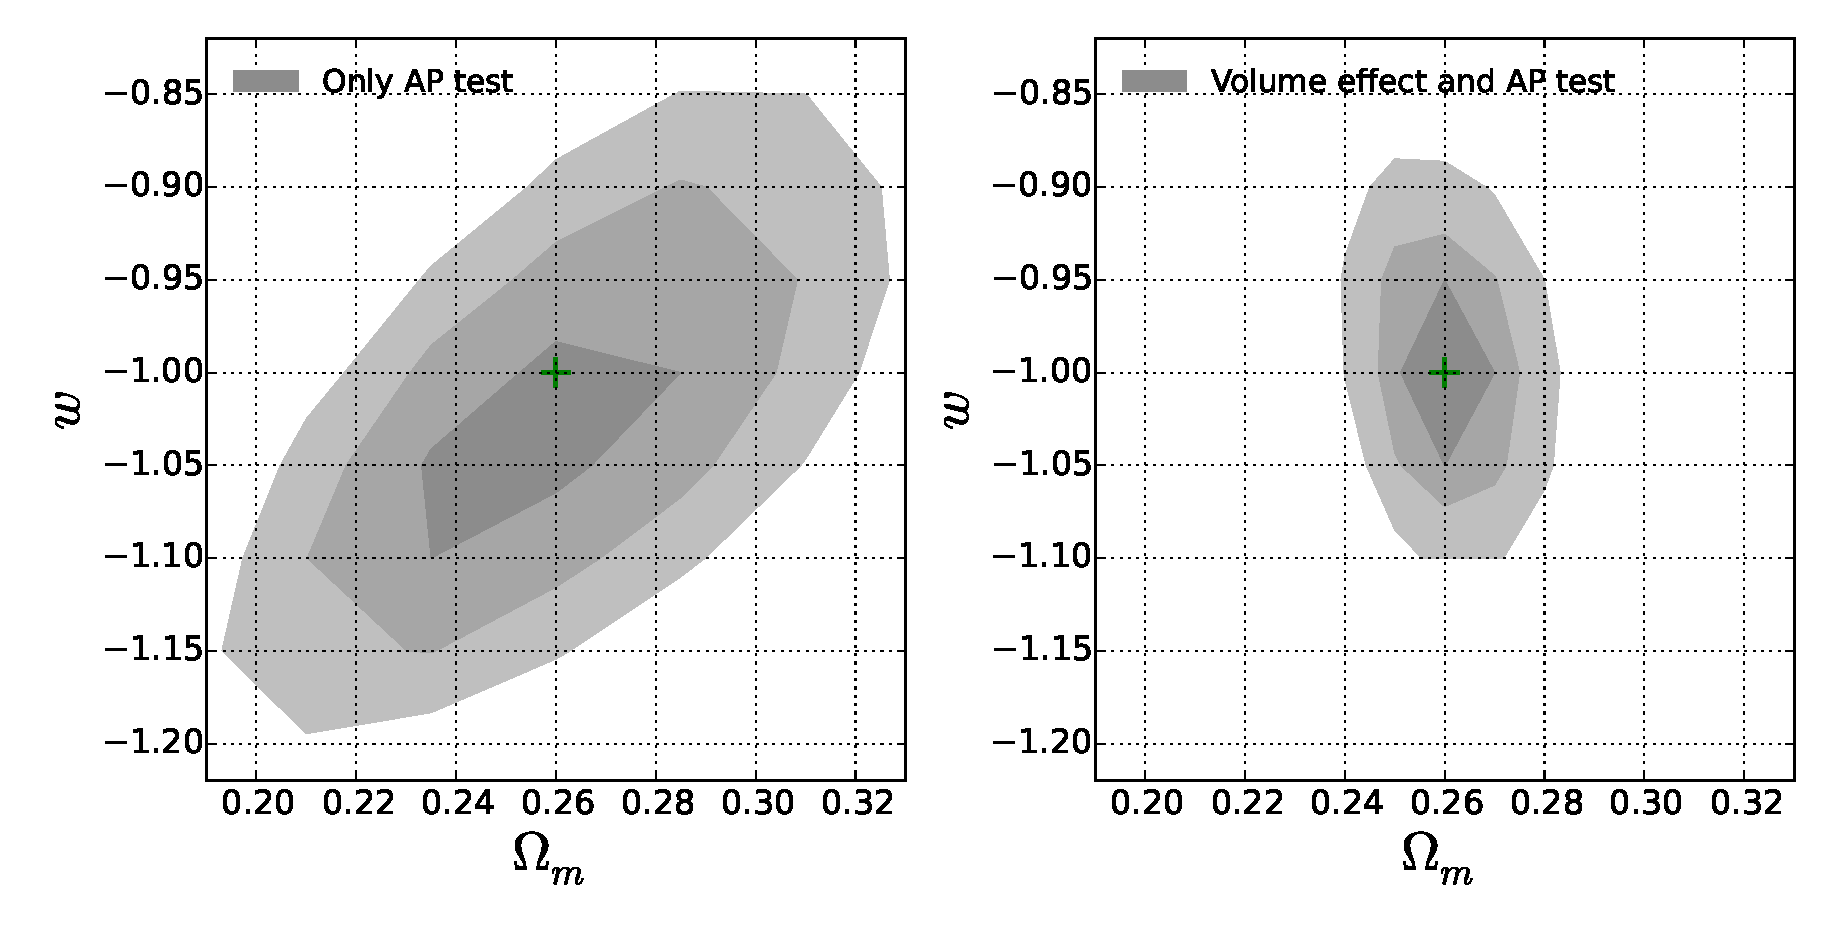
\includegraphics[width=7cm]{Tpcf--contour.eps}
   %\includegraphics[width=16cm]{Tpcf--contour-others.eps}
   %\includegraphics[width=16cm,natwidth=52,natheight=40]{fig10.eps}
   %\includegraphics[width=16cm]{fig10.eps}
   }
   \caption{\label{fig}
   Likelihood contours (68.3\%, 95.4\%) in the $\Omega_m-w$ plane from our method.
   }
\end{figure*}

In this analysis we simply assume flat priors for $\Omega_m$ and $w$,
and approximate $P({\bf D}|{\bf \theta})$ by a likelihood function $\mathcal{L}$
satisfying  $-2 \ln \mathcal{L}=\chi^2$;
the PDF of $\theta$ derived from our AP method takes the form
%The PDF cu is approximated by the {\it likelihood} function of $\mathcal{L}\propto \exp\left(-\frac{\chi^2}{2}\right)$.
%It is approximated by the {\it likelihood} function.
%So we have
\begin{equation}
 P({\bf \theta}|{\bf D}) \propto \mathcal{L} \propto \exp\left[-\frac{\chi^2}{2}\right].
\end{equation}
We use the {\texttt {COSMOMC}} software \citep{LB2002}
to obtain the Markov Chain Monte Carlo (MCMC) samples of $\theta$ following the PDF of $P({\bf \theta}|{\bf D})$.
Constraints on $\Omega_m$ and $w$ are derived from these samples.

The 68\% and 95\% likelihood contours of $\Omega_m$ and $w$ 
obtained from this analysis are shown in Figure \ref{fig_contours} (pink areas).
%For comparison, results from some other cosmological probes are also plotted.
Our AP method yields tight constraints on $\Omega_m$ and $w$ .
The mean values and 68\% CL are
\begin{equation}
 \Omega_m=0.314 \pm 0.038,\ \ w = -1.09 \pm 0.14.
\end{equation}
This result is consistent with the Planck $\Lambda$CDM cosmology within 1$\sigma$ \citep{Planck2015}.


%\bibitem[Blake et al. (2011)]{WiggleZB}
%Blake, C., Kazin, E.A., Beutler, F., et al.
%2011, MNRAS, 418, 1707
%\bibitem[Kazin et al. (2014)]{WiggleZK}
%Kazin, E.A., Koda, J., Blake, C., et al.
%2014, MNRAS, 441, 352





\section{Concluding Remarks}

 * Can be combined with our redshift dependence of AP to full explore the geometric effects in LSS

 * *** utilizes angular 2pCF as a function of redshift. Our method is complementary to it: 1) smaller scales; 2) more bins; 3) could be less affected by RSD; ... In case of good modelling of RSD one can rely on their; in case not possible, especially on small scales, one can use ours

 * Complementary to all other LSS probes

 * Promising future



\section*{Acknowledgments}

We thank the Korea Institute for Advanced Study for providing computing resources (KIAS Center for Advanced Computation Linux Cluster System).
%We thank Seokcheon Lee and Graziano Rossi for many helpful discussions.
We would like to thank Yi Zheng for useful discussions.
This work was partially supported by the
Supercomputing Center/Korea Institute of Science and
Technology Information with supercomputing resources
including technical support (KSC-2013-G2-003).


\appendix

\

\begin{thebibliography}{}

\bibitem[Ade et al. (2015)]{Planck2015}
Ade, P.A.R., Aghanim, N., \& Arnaud, M., et al. arXiv:1502.01589

\bibitem[Alam et al.(2016)]{Alam2016}
Alam, S., Ata, M., \& Bailey, S., et al. 2016,
submitted to MNRAS (arXiv:1607.03155)

\bibitem[{{Alam} {et~al}\mbox{.}(2015{\natexlab{a}}){Alam}, {Albareti},
  {Allende Prieto}, {Anders}, {Anderson}, {Anderton}, {Andrews}, {Armengaud},
  {Aubourg}, {Bailey}, \& et~al.}]{dr12}
{Alam} S., Albareti, F.D.,\& Allende Prieto, C., {et~al.}, 2015,  ApJS, 219, 12

\bibitem[Alcock \& Paczynski(1979)]{AP1979}
Alcock, C., \& Paczynski, B. 1979, Nature, 281, 358  

%\bibitem[Anderson et al.(2012)]{2012MNRAS.427.3435A} 
%Anderson, L., Aubourg, E., Bailey, S., et al.\ 2012, MNRAS, 427, 3435

\bibitem[Anderson et al.(2013)]{Anderson2013}
Anderson, L., Aubourg, \'E., \& Bailey, S. et al. 2014, MNRAS, 441, 24  
  
%\bibitem[Bassett et al.(2002)]{Bassett2002}
%Bassett, B.A., Kunz, M., Silk, J., \& Ungarelli, C. 2002, MNRAS, 336, 1217

\bibitem[Ballinger, Peacock \& Heavens 1996]{Ballinger1996}
Ballinger, W.E., Peacock, J.A., \& Heavens, A.F. 1996, MNRAS, 282, 877  

\bibitem[Betoule et al.(2014)]{JLA}
Betoule, M., Kessler, R., \& Guy, J., et al. 2014, A\&A, 568, 32


\bibitem[Beutler et al.(2011)]{6dFGS}
Beutler, F., Blake, C., \& Colless, M., et al. 2011, MNRAS, 416, 3017

\bibitem[Beutler et al.(2013)]{Beutler2013}
Beutler, F., Saito, S., \& Seo, H.-J., et al. 2013, MNRAS, 443, 1065

\bibitem[Beutler et al.(2016)]{Beutler2016}
Beutler, F., Seo, H.-J., \& Saito, S., et al. 2016,
arXiv:1607.03150

\bibitem[Blake et al.(2011)]{Blake2011}
Blake, C., Glazebrook, K., \& Davis, T. M., 2011, MNRAS, 418, 1725  

\bibitem[Blake et al.(2013)]{WiggleZtopoloy}
Blake, C., James, J.B., \& Poole, G.B. 2013, MNRAS, 437, 2488

\bibitem[Bolton et al.(2012)]{Bolton2012}
Bolton, A.S., Schlegel, \& D.J., Aubourg E., et al. 2012, AJ, 144, 144

\bibitem[Boylan-Kolchin et al.(2008)]{B08}
Boylan-Kolchin, M., Ma, C.-P., \& Quataert, E. 2008, MNRAS, 383, 93


%\bibitem[Bueno Belloso et al. (2012)]{BB2012}
%Bueno Belloso, A., Pettinari, G.W., Meures, N., \& Percival, W.J. 2012, Phys. Rev. D, 86, 023530

%\bibitem[Chevallier \& Polarski(2001)]{CP2001}
%Chevallier, M., Polarski, D. 2001, Int. J. Mod. Phys. D, 10, 213


%\bibitem[Choi et al.(2010)]{choi 2010}
%Choi, Y.-Y., Park, C., Kim, J., Gott, J.R., 
%Weinberg, D.H., Vogeley, M.S., \& Kim, S.S. 2010, ApJS, 190, 181

\bibitem[Christensen et al.(2001)]{Bayesian}
Christensen, N., Meyer, R., Knox, L., \& Luey, B. 2001, Class. Quant. Grav., 18, 2677

%\bibitem[Chuang et al.(2013)]{Chuang2013}
%Chuang, C.-H., Prada, F., Beutler, F., et al. 2013, arXiv:1312.4889  

\bibitem[Chuang \& Wang(2012)]{ChuangWang2012}
Chuang, C.-H., \& Wang, Y. 2012, MNRAS, 426, 226  


%\bibitem[Corasaniti \& Copeland(2003)]{Corasaniti2003}
%Corasaniti, P.S., Copeland, E.J. 2003, Phys. Rev. D, 67, 063521

%eBOSS: 
%http://arxiv.org/abs/1508.04473
\bibitem[Dawson et al.(2015)]{eBOSS}
Dawson, K.S., Kneib, J.P., \& Percival, W.J., et al. 2015, accepted AJ

\bibitem[Dawson et al.(2012)]{Dawson et al. 2012}
Dawson, K.S., Schlegel, D.J., \& Ahn, C.P., et al. 2012, AJ, 145, 10

\bibitem[Efstathiou (2014)]{E14H0}
Efstathiou, G. 2014, MNRAS, 440, 1138

\bibitem[Eisenstein et al.(2011)]{Eisenstein et al. 2011}
Eisenstein, D.J.,  Weinberg, D.H., \& Agolet, E., et al. 2011, AJ, 142, 72

\bibitem[Feldman, Kaiser \& Peacock (1994)]{1994ApJ...426...23F} 
Feldman, H.A., Kaiser, N., \& Peacock, J.A.\ 1994, ApJ, 426, 23 

\bibitem[Fukugita et al. (1996)]{Fukugita1996}
Fukugita, M., Ichikawa, T., \& Gunn, J.E., et al. 1996, AJ, 111, 1748
%Publication:	
%Astronomical Journal v.111, p.1748 

%\bibitem[Gingold \& Monaghan(1977)]{GM1977}
%Gingold, R.A., \& Monaghan, J.J. 1977, MNRAS, 181, 375  

%\bibitem[Gott et al.(2009)]{gott 2009}
%Gott, J.R., Choi, Y.-Y., Park, C., \& Kim, J. 2009, ApJ, 695, L45  

%\bibitem[Gott et al.(2008)]{gott 2008}
%Gott, J.R., Hambrick, D.C., Vogeley, M.S., Kim, J., Park, C., Choi, Y.-Y.,
%Cen, R., Ostriker, J.P., \& Nagamine, K. 2008, ApJ, 675, 16  


\bibitem[Gunn et al. (1998)]{Gunn1998}	
Gunn, J.E., Carr, M., \& Rockosi, C. et al. 1998, AJ, 116, 3040

\bibitem[Gunn et al.(2006)]{Gunn et al. 2006}
Gunn, J.E., Siegmund, W.A., \& Mannery, E.J., et al. 2006, AJ, 131, 2332

\bibitem[Guzzo et al.(2008)]{Guzzo2008}
Guzzo, L., Pierleoni, M., \& Meneux, B., et al. 2008, Nature, 451, 541

\bibitem[Hartlap et al.(2006)]{Hartlap}
Hartlap J., Simon P. \& Schneider P. [astro-ph/0608064].


\bibitem[Hong et al.(2016)]{hong2016}
Hong, S.E., Park, C.,\&  Kim, J. 2016, ApJ, 823, 103

\bibitem[Jackson (1972)]{FOG}
Jackson, J., 1972, MNRAS, 156, 1

\bibitem[Jennings et al.(2011)]{Jennings2011}
Jennings, E., Baugh, C.M., \& Pascoli, S. 2011, MNRAS, 420, 1079  

%\bibitem[Jeong et al.(2014)]{Jeong2014}
%Jeong, D., Dai, L., Kamionkowski, M., \& Szalay, A.S. 2014, arXiv:1408.4648

\bibitem[Jiang et al.(2008)]{jiang2008}
Jiang, C.Y., Jing, Y. P., \& Faltenbacher, A., et al. 2008, ApJ, 675, 1095

\bibitem[Kaiser (1987)]{Kaiser1987}
Kaiser, N. 1987, MNRAS, 227, 1


\bibitem[Kim \& Park(2006)]{kim and park 2006}
Kim, J., \& Park, C. 2006, ApJ, 639, 600  

\bibitem[Kim et al.(2009)]{2009ApJ...701.1547K} 
Kim, J., Park, C., Gott, J.R., III, \& Dubinski, J.\ 2009, ApJ, 701, 1547 

\bibitem[Kim et al.(2015)]{hr4}
Kim, J., Park, C., L'Huillier, B., \& Hong, S. E. 2015, JKAS, 48, 213

\bibitem[Kim et al.(2011)]{horizonrun}
Kim, J., Park, C., Rossi, G., Lee, S.M., \& Gott, J.R. 2011, JKAS, 44, 217  

\bibitem[Kitaura et al.(2015)]{MDPATCHY}
Kitaura, F.S., Rodrı\'{i}guez-Torres, S., Chuang, C.-H., et al. arXiv:1509.06400

\bibitem[Komatsu et al.(2011)]{komatsu 2011}
Komatsu, E., Smith, K. M., \& Dunkley, J., et al. 2011, ApJS, 192, 18  

\bibitem[Lacey \& Cole(1993)]{LC93}
Lacey, C., \& Cole, S. 1993, MNRAS, 262, 627


\bibitem[Landy \& Szalay(1993)]{1993ApJ...412...64L} 
Landy, S.D., \& Szalay, A.S.\ 1993, ApJ, 412, 64 

%EUCLID:
%http://arxiv.org/abs/1110.3193
\bibitem[Laureijs et al.(2011)]{EUCLID}
Laureijs, R., Amiaux, J., \& Arduini, S., et al. 2011, arXiv:1110.3193

\bibitem[Lavaux \& Wandelt(2012)]{LavausWandelt1995}
Lavaux, G., \& Wandelt, B.D. 2012, ApJ, 754, 109  

%\bibitem[Levi et al.(2013)]{2013arXiv1308.0847L} 
%Levi, M., Bebek, C., Beers, T., et al.\ 2013, arXiv:1308.0847 

\bibitem[Lewis \& Bridle (2002)]{LB2002}
Lewis, A., \& Bridle, S. 2002, Phys. Rev. D, 66, 103511

\bibitem[L'Huillier et al.(2014)]{2014NewA...30...79L} 
L'Huillier, B., Park, C., \& Kim, J.\ 2014, New Astronomy, 30, 79 

\bibitem[Li et al.(2011)]{Li2011}
Li, M., Li, X.-D., Wang, S., \& Wang, Y. 2011, Commun. Theor. Phys., 56, 525

\bibitem[Li et al.(2014)]{Li2014}
Li, X.-D., Park, C., Forero-Romero, J., \& Kim, J. 2014, ApJ, 796, 137

\bibitem[Li et al.(2015)]{Li2015}
Li, X.-D., Park, C., Sabiu, C.G., \& Kim, J. 2015, MNRAS, 450, 807 

\bibitem[Li et al.(2016)]{Li2016}
Li, X.-D., Park, C., Sabiu, C.G., \& Kim, J. 2016, submitted to ApJ


%\bibitem[Linder(2003)]{Linder2003}
%Linder, E.V. 2003, Phys. Rev. Lett., 90, 091301

\bibitem[Linder et al.(2014)]{Linder2013}
Linder, E.V., Minji, O., Okumura, T., Sabiu, C.G., \& Song, Y.-S. 2014, Phys. Rev. D, 89, 063525  

\bibitem[L{\'o}pez-Corredoira(2014)]{2014ApJ...781...96L} 
L{\'o}pez-Corredoira, M.\ 2014, ApJ, 781, 96 

\bibitem[Marinoni \& Buzzi(2010)]{Marinoni2010}
Marinoni, C., \& Buzzi, A. 2010, Nature, 468, 539  

\bibitem[Matsubara \& Suto(1996)]{Matsubara1996}
Matsubara T., \& Suto, Y. 1996, ApJ, 470, L1  

\bibitem[McCavana et al.(2012)]{M12}
McCavana, T., Micic, M., Lewis, G. F., et al. 2012, MNRAS, 424, 361


\bibitem[Morandi \& Sun (2016)]{MS2016}
Morandi, A., \& Sun, M. arXiv:1601.03741


\bibitem[Outram et al.(2004)]{Outram2004}
Outram, P.J., Shanks, T., Boyle, B.J., Croom, S.M., Hoyle, F., Loaring, N.S., 
Miller, L., \& Smith, R.J. 2004, MNRAS, 348, 745  

%\bibitem[Parejko et al.(2013)]{Parejko2013}
%Parejko, J. K., Sunayama, T., Padmanabhan, N., et al. 2013, MNRAS, 429, 98  

\bibitem[Parejko et al.(2013)]{Parejko2013}
Parejko J.K., et al., 2013, MNRAS, 429, 98

\bibitem[Parihar et al. (2014)]{CMASSLSS2014}
Parihar, P., Vogeley, M.S., \& Gott, J.R., et al. 2014, ApJ, 796, 86

\bibitem[Park et al.(2005)]{park 2005}
Park, C., Kim, J., \& Gott, J.R. 2005, ApJ, 633, 1  

\bibitem[Park \& Kim(2010)]{topology}
Park, C., \& Kim, Y.-R. 2010, ApJL, 715, L185  

\bibitem[Park et al. (2012)]{Park2012}
Park, C., Choi, Y.-Y., Kim, J., Gott, J.R., Kim, S.S., \&
Kim, K.-S. 2012, ApJ, 759, 7

\bibitem[Park et al. (2015)]{Park2015}
Park, C., Song, H., Einasto, M., Lietzen, H., \&
Heinamaki, P. 2015, JKAS, 48, 75

\bibitem[Peebles \& Ratra(2003)]{PR2003}
Peebles, P.J.E., \& Ratra, B. 2003, Reviews of Modern Physics, 75, 559

\bibitem[Percival et al.(2014)]{Percival2014}
Percival, W.J., Ross, A.J., \& S\'{a}nchez, A.G., et al. 2014, MNRAS, 439, 2531

\bibitem[Perlmutter et al.(1999)]{Perl1999}
Perlmutter, S., Aldering, G., \& Goldhaber, G., et al. 1999, ApJ, 517, 565  

\bibitem[Press \& Shechter(1974)]{PS1974}
Press, W.H., \& Schechter, P.L. 1974, ApJ, 187, 425

\bibitem[Reid et al.(2012)]{Reid2012}
Reid, B., Samushia, L., \& White, M., et al. 2012, MNRAS, 426, 2719  

\bibitem[Reid et al.(2016)]{Reidetal:2016}
Reid, B., Ho, S., \& Padmanabhan, N., et al.  2016, MNRAS, 455, 1553

\bibitem[Riess et al.(1998)]{Riess1998}
Riess, A.G., Filippenko, A.V., \& Challis, P., et al. 1998, AJ, 116, 1009  

\bibitem[Riess et al.(2011)]{Riess2011}
Riess, A.G., Macri, L., \& Casertano, S., et al. 2011, ApJ, 730, 119
%A 3\% Solution: Determination of the Hubble Constant with the Hubble Space Telescope and Wide Field Camera

\bibitem[Ross et al.(2012)]{2012MNRAS.424..564R} 
Ross, A.J., Percival, W.J., \& S{\'a}nchez, A.G. et al.\ 2012, MNRAS, 424, 564 

\bibitem[Ross et al.(2015)]{MGS}
Ross, A.J., Samushia, L., \& Howlett, C., et al. 2015, MNRAS, 449, 835

\bibitem[Ryden(1995)]{Ryden1995}
Ryden, B.S. 1995, ApJ, 452, 25  

%\bibitem[Samushia et al.(2014)]{Samushia2014}
%Samushia, L., Reid, B. A., White, M., et al. 2014, MNRAS, 439, 3504  

%\bibitem[Sanchez et al.(2013)]{Sanchez2013}
%Sanchez, A. G., Kazin, E. A., Beutler, F., et al. 2013, MNRAS, 433, 1202  

%\bibitem[Sutter et al.(2014)]{Sutter2014}
%Sutter, P.M., Pisani, A., Wandelt, B.D., \& Weinberg, D.H. 2014, MNRAS, 443, 2983


\bibitem[Sanchez et al.(2016)]{Sanchez2016}
Sanchez, A. G., Scoccimarro, R., \& Crocce, M., et al.
arXiv:1607.03147

\bibitem[Schlafly et al.(2010)]{Schlafly2010}
Schlafly E.F., Finkbeiner D.P., Schlegel D.J., et al. 2010, ApJ, 725, 1175

\bibitem[Schlafly \& Finkbeiner(2011)]{SF2011}
Schlafly E.F., \& Finkbeiner D.P. 2011, ApJ, 737, 103


%DESI:
%http://arxiv.org/abs/1106.1706
\bibitem[Schlegel et al.(2011)]{DESI}
Schlegel, D., Abdalla, F., \& Abraham, T., et al. 2011, arXiv:1106.1706

\bibitem[Smee et al.(2013)]{Smee2013}
Smee, S.A., Gunn, J.E., \& Uomoto, A., et al. 2013, AJ, 146, 32

\bibitem[Song et al.(2014)]{2014arXiv1407.2257S} 
Song, Y.S., Sabiu, C.G., 
Okumura, T., Oh, M., \& Linder, E.V.\ 2014, JCAP, 12, 005 

\bibitem[Speare et al. (2015)]{Speare2015}
Speare, R., Gott, J.R., Kim, J., \& Park, C.
2015, ApJ, 799, 176

%\bibitem[Tojeiro \& Percival(2011)]{Tojeiro2011}
%Tojeiro R., \& Percivial W.J. 2011, MNRAS, 417, 1114  

%\bibitem[Tojeiro et al.(2012)]{Tojeiro2012}
%Tojeiro, R., Percival, W. J., Wake, D. A., et al. 2012, MNRAS, 424, 136 

\bibitem[Viana \& Liddle(1996)]{VL1996}
Viana, P.T.P., \& Liddle, A.R. 1996, MNRAS, 281, 323

\bibitem[Villalobos et al.(2013)]{V13}
Villalobos, \'{A}., ́De Lucia, G., Weinmann, S.M., Borgani, S., \& Murante, G. 2013, MNRAS, 433, L49


\bibitem[Weinberg (1989)]{SW1989}
Weinberg, S. 1989, Reviews of Modern Physics, 61, 1

\bibitem[White (2011)]{White2011}
White M., et al. 2011, ApJ, 728, 126

\bibitem[York et al.(2000)]{York et al. 2000}
York, D.G., Adelman, J., \& Anderson, J.E., et al. 2000, AJ, 120, 1579

\bibitem[Zehavi et al.(2011)]{zehavi2011}
Zehavi, I., Zheng, Z., \& Weinberg, D.H., et al. 2011, ApJ, 736, 59




\end{thebibliography}


\end{document}
